\documentclass{ituthesis}

\settitle{Copatterns in Idris}
\setauthor{Sune Alk\ae rsig \& Thomas Hallier Didriksen}
\setsupervisor{Peter Sestoft}
\setextrasupervisor{David Christiansen}
\setdate{March 2015}

\usepackage{float}
\usepackage[utf8]{inputenc}
\usepackage{url}
\usepackage{alltt}
\usepackage{amssymb, amsfonts, amsmath, amsthm}
\usepackage{mathtools}
\usepackage{listings}
\usepackage{natbib}
\usepackage{pdflscape}
\usepackage{todonotes}
\bibliographystyle{alpha}
\usepackage{semantic}
\usepackage{fullpage}
\usepackage[normalem]{ulem}
\usepackage{caption}
\usepackage{subcaption}
\usepackage{bussproofs}
 % Macros to get display-style math in proof trees.
  \newcommand{\AXD}[1]{\AxiomC{\ensuremath{\displaystyle #1}}}
  \newcommand{\UID}[1]{\UnaryInfC{\ensuremath{\displaystyle #1}}}
  \newcommand{\BID}[1]{\BinaryInfC{\ensuremath{\displaystyle #1}}}
  \newcommand{\TID}[1]{\TrinaryInfC{\ensuremath{\displaystyle #1}}}
  \newcommand{\QID}[1]{\QuaternaryInfC{\ensuremath{\displaystyle #1}}}
  \newcommand{\RLabel}[1]{\RightLabel{\ensuremath{#1}}}

\newcommand{\IdrisM}{Idris$^{-}$}
\newcommand{\later}{\rhd}
% Kappa commands
\newcommand{\onk}[1]{#1^\kappa}
\newcommand{\laterkappa}{\later^{\!\!\kappa}}
\newcommand{\laterkappan}{\later^{\!\!\kappa}_{\!\! n}}
\newcommand{\laterk}[1]{\later^{\!\!\!\kappa}#1^\kappa}
\newcommand{\forallk}[1]{\forall\kappa.#1^\kappa}
\newcommand{\flaterk}[1]{\forall\kappa.\later^{\!\!\!\kappa}#1^\kappa}
% Kappa prime commands
\newcommand{\onkp}[1]{#1^\kappa'}
\newcommand{\laterkappap}{\later^{\!\!\!\kappa'}}
\newcommand{\laterkp}[1]{\later^{\!\!\!\kappa'}#1^{\kappa'}}
\newcommand{\forallkp}[1]{\forall\kappa'.#1^{\kappa'}}
\newcommand{\flaterkp}[1]{\forall\kappa'.\later^{\!\!\!\kappa'}#1^{\kappa'}}
\newcommand{\tensor}{\circledast}
\newcommand{\tensorkappan}{\ensuremath{\tensor^\kappa_n}}
\newcommand{\clockEnv}{\ensuremath{\Delta}}

\newcommand{\quine}[1]{\ensuremath{\ulcorner}#1\ensuremath{\urcorner}}
\newcommand{\eps}[6]{\ensuremath{#1\,\vdash\,#2\,:\,#3\,\xRightarrow{#6}\,#4\,\vdash\,#5\,:\,#6}}
\newcommand{\causal}{\ensuremath{\curvearrowleft}}
\newcommand{\noncausal}{\ensuremath{\leftrightarrows}}
\newcommand{\open}{\ensuremath{\sqcup}}
\newcommand{\closed}{\ensuremath{\sqcap}}
\newcommand{\infer}{\ensuremath{\Longrightarrow}}
\newcommand{\IEopen}{\ensuremath{\iota;\Psi;\phi;\open;\Gamma}}
\newcommand{\IEclosed}{\ensuremath{\iota;\Psi;\phi;\closed;\Gamma}}
\newcommand{\IEc}{\ensuremath{\iota;\Psi;\phi;\clockEnv;\Gamma}}
\newcommand{\IEopencausal}{\ensuremath{\iota;\causal;\phi;\open;\Gamma}}
\newcommand{\IEclosedcausal}{\ensuremath{\iota;\causal;\phi;\closed;\Gamma}}
\newcommand{\IEopennoncausal}{\ensuremath{\iota;\noncausal;\phi;\open;\Gamma}}
\newcommand{\IEclosednoncausal}{\ensuremath{\iota;\noncausal;\phi;\closed;\Gamma}}

\newcommand{\CEc}{\ensuremath{\iota; \Psi; \clockEnv; \Gamma}}
\newcommand{\CEclosed}{\ensuremath{\iota; \Psi; \closed; \Gamma}}
\newcommand{\CEclosedcausal}{\ensuremath{\iota; \causal; \closed; \Gamma}}
\newcommand{\CEclosednoncausal}{\ensuremath{\iota; \noncausal; \closed; \Gamma}}
\newcommand{\CEopen}{\ensuremath{\iota; \Psi; \open; \Gamma}}
\newcommand{\CEopencausal}{\ensuremath{\iota; \causal; \open; \Gamma}}
\newcommand{\CEopennoncausal}{\ensuremath{\iota; \noncausal; \open; \Gamma}}

%\lstset{basicstyle=\ttfamily}

% Theorem Styles
\newtheorem{theorem}{Theorem}[section]
\newtheorem{lemma}[theorem]{Lemma}
\newtheorem{proposition}[theorem]{Proposition}
\newtheorem{corollary}[theorem]{Corollary}
% Definition Styles
\theoremstyle{definition}
\newtheorem{definition}{Definition}[section]
\newtheorem{example}{Example}[section]
\theoremstyle{remark}
\newtheorem{remark}{Remark}

\begin{document}

\frontmatter

\thetitlepage
\newpage

\chapter*{Abstract}
This is an abstract

\cleardoublepage
\setcounter{tocdepth}{1}
\tableofcontents

\mainmatter
\midsloppy
\sloppybottom

%!TEX root = ../copatterns-thesis.tex
\chapter{Introduction}

%!TEX root = ../copatterns-thesis.tex
\chapter{Background}

% Sune
%#############
% Hvad er copatterns?
% Hvorfor giver copatterns mening, isoleret set?
% Hvor kommer copatterns fra? (Hagino, Abel og venner)
% Definition ved observation (eliminationsregler)
% Eksempler

% Ny viden: Copatterns
%#############

\section{Copatterns}
\label{sec:copatterns}
In functional programming, inductive data is commonly defined by \emph{constructors} in an
elegant and simple fashion. The data can be analyzed and manipulated using
pattern matching, which follows nicely from the finite nature of inductive
data. The growing consensus\todo{Among who?} is that coinductive data should be defined by
\emph{observations} due to its possible infinity. This\todo{Perhaps say this at
  the beginning?} means that one should distingush
between finite and infinite data. Hagino\todo{Hagino introduced a construct for
  synthesizing coinductive data. The distinction between finite and infinite
  data was already known.} first introduced this idea in his SymML
language \,\citep{Hagino89}, where the programmer could define coinductive types
by their \emph{destructors} or \emph{observations}. In other words\todo{We have
  to be precise here. }, inductive
types should be defined by their \emph{introduction rules}, and coinductive types by
their \emph{elimination rules}.

\begin{figure}[h]
\begin{lstlisting}[mathescape]
corecord Stream : Type -> Type where
  head : Stream a -> a
  tail : Stream a -> Stream a 
  constructor MkStream
\end{lstlisting}
\caption{An infinite list defined by observations.}
\label{fig:stream}
\end{figure}

The syntax for \texttt{codata} definitions presented in
Figure~\ref{fig:stream} defines a coinductive type by observations, as oppose to
by constructors. On a \texttt{Stream}, two observations can be made:
\texttt{head} and \texttt{tail}. The former provides us with the first element
of the stream, while the latter gives us with the rest of the infinite stream,
upon which another element can be observed with \texttt{head}. 

\emph{Destructor copatterns}, or simply
\emph{copatterns}\,\citep{Abel13Copatterns}, provide a way of defining functions
on coinductive data in terms of observations. Like pattern matching allows us to
define functions on inductive data by analyzing the structure of the input,
copatterns enable us to make experiments on functions with a result of
coinductive type.

The \texttt{Stream} defined by observations can be used to define a function
\texttt{nats}, an list of all natural numbers, using copatterns, as shown in
Figure~\ref{fig:nats_copatterns}.


\begin{figure}[h]
\begin{lstlisting}[mathescape]
nats : Stream Nat
head nats = Z
tail nats = map S nats
\end{lstlisting}
\caption{A definition of \texttt{nats} using copatterns.}
\label{fig:nats_copatterns}
\end{figure}

Because the result type of \texttt{nats} is defined by observations, we can use
copatterns to define the outcomes of our observations. The intuition is that the
first element of \texttt{nats} is zero (\texttt{Z}), and the rest of the natural
numbers are all the natural numbers incremented by one (\texttt{map S
  nats}). Initially, the \texttt{head} observation will therefore return
\texttt{Z}. Making a \texttt{tail} observation results in a new stream where all
the elements of \texttt{nats} are incremented by one (using the \texttt{S}
constructor for natural numbers). Consequently, the outcome of making a
subsequent \texttt{head} observation is \texttt{S Z}. As we can increment a
natural number infinitely many times, we can also make infinitely many
\texttt{tail} observations, where the result of a \texttt{head} observation will
be incremented for each \texttt{tail} observation. 


Syntactically, projection happens on the outside of definitions when we use
copatterns, as opposed to pattern matching, where projection on parameters
happens inside of definitions. As an example, consider the definition of
\texttt{map} in Figure~\ref{fig:map_copatterns}.

\begin{figure}[h]
\begin{lstlisting}[mathescape]
map : (a -> b) -> Stream a -> Stream b
head (map f s) = f (head s)
tail (map f s) = map f (tail s)
\end{lstlisting}
\caption{The \texttt{map} function defined with copatterns.}
\label{fig:map_copatterns}
\end{figure}

For \texttt{map}, it is clear that the observations are applied on the entire
definition \texttt{map f s}. Projections on the entire definition make sense
because \texttt{map f s} has the coinductive type \texttt{Stream b}, which can
be the subject of observations. In this sense, copatterns can be said to be dual
to pattern matching in the same way that coinductive data is dual to inductive
data. With pattern matching, we can analyze how data has been constructed, and
with copatterns we can define the outcome of observations. Where pattern
matching is a way of processing input, copatterns provide the means for
describing output. 

\subsection{The Anatomy of Copatterns}
\todo{Establish names for different parts of a definition with copatterns here:
  In particular, we need to define the following: clause, pattern clause, pattern,
  argument pattern, copattern clause, copattern, left-hand side projection,
  observation, and probably more}

\subsection{Existing Implementations of Copatterns}
Copatterns already exist in programming languages, for example in
Agda\,\cite{Norell:thesis}. Here, definitions for coinductive types are quite
interesting. A coinductive type is defined as a record type with a
\texttt{coinductive} flag, an example of which can be seen in
Figure~\ref{fig:agda_stream}. Observations are defined as fields of the record
type.

\begin{figure}[h]
\begin{lstlisting}[mathescape]
record Stream (A : Set) : Set where
  coinductive
  field
    head : A
    tail : Stream A
open Stream
\end{lstlisting}
\caption{\texttt{Stream} definition in Agda.}
\label{fig:agda_stream}
\end{figure}

Definitions with copatterns are almost identical to what has already been
discussed. A simple example \texttt{repeat} in Figure~\ref{fig:agda_repeat}. 

\begin{figure}[h]
\begin{lstlisting}[mathescape]
repeat : {A : Set} -> A -> Stream A
head (repeat a) = a
tail (repeat a) = repeat a 
\end{lstlisting}
\caption{A corecursive \texttt{repeat} function in Agda.}
\label{fig:agda_repeat}
\end{figure}

In Section\,\ref{sec:motivation_copatterns} we discuss the motivation behind the
use of copatterns. Later, in Chapter\,\ref{sec:adding_copatterns}, we describe
how we have added a syntax for copatterns and for defining coinductive types by
their observations (\texttt{corecord}s) to the programming language Idris. The
syntax we have added to Idris includes a prefix character, \texttt{\&}, on the
observation patterns, an example of which you can see in
Figure~\ref{fig:map_copat_syntax}. In the remaining report we will use this
syntax for copattern definitions.

\begin{figure}[h]
\begin{lstlisting}[mathescape]
map : (a -> b) -> Stream a -> Stream b
&head (map f s) = f (head s)
&tail (map f s) = map f (tail s)
\end{lstlisting}
\caption{The \texttt{map} function defined with copatterns using the syntax
  described in Chapter~\ref{sec:adding_copatterns}.}
\label{fig:map_copat_syntax}
\end{figure}

%%% Local Variables: 
%%% mode: latex
%%% TeX-master: "../../copatterns-thesis"
%%% End: 

\section{Syntactic Guardedness}

%%% Local Variables: 
%%% mode: latex
%%% TeX-master: "../../copatterns-thesis"
%%% End: 

%!TEX root = ../../copatterns-thesis.tex
\section{Guarded Recursion}
\label{sec:guarded-recursion}

Guarded recursion provides a typing discipline which ensures that all programs adhering to their type specification must be productive. In a system with a syntactic guardedness condition, the productivity of a given program follows from its syntactic structure. With guarded recursion, the productivity of a program follows from its type. Consequently, it is impossible to write a well-typed guarded recursive program which is not productive.

\subsection{The Guardedness Type Constructor}
The use of guarded recursion was pioneered by Nakano\,\citep{Nakano:2000}, who presented a type system (based on $\lambda \mu$) where no well-typed terms diverge by introducing a guardedness type constructor for a type $A$, $\later A$, into the type system. Although Nakano does not call it so explicitly, we recommend that the guardedness type constructor $\later$ is read as ``later''. The addition of the $\later$ operator leads to a type system where there is a distinction between an inhabitant of a type $A$, which must be available now (i.e. at any point in time), and an inhabitant of $\later A$, which is available later (i.e. not now). Using this intuition, a stream of elements of type $A$ can be defined as described in Figure\,\ref{fig:guarded_recursion_stream}. The idea is that we can access the head of the stream now, but we cannot access the recursive reference in the tail until later.

\begin{figure}
\[
Stream\,A = \mu X. A \times \later X
\]
\[
\frac{\Gamma\vdash x : A \quad \quad \Gamma\vdash s : \later Stream\,A}{\Gamma\vdash StreamCons(x,s) : Stream\,A} StreamCons
\]
\[
\frac{\Gamma\vdash s : Stream\,A}{\Gamma\vdash hd(s) : A} hd
\]
\[
\frac{\Gamma\vdash s : Stream\,A}{\Gamma\vdash tl(s) : \later Stream\,A} tl
\]
\caption{A guarded recursive definition of streams, along with introduction and elimination rules.}
\label{fig:guarded_recursion_stream}
\end{figure} 

%At this point, we can draw a parallel to syntactic guardedness. Since any manipulation of recursive references is disallowed, syntactic guardedness essentially requires that recursive references are also available now, because there is no guarantee that a result can be given at any later point in time. In contrast, any guarded recursive definition must guarantee that even though the recursive reference is manipulated, a result will always be available later.

\subsection{Constructing Guarded Recursive Programs}
\label{sec:constr-guard-recurs}
To obtain the guarantees of productivity provided by guarded recursion, guarded recursive programs must be constructed in a special way. For this purpose, Nakano defines a guarded fixpoint operator, shown in Figure\,\ref{fig:guarded_recursion_fixpoint}. As the recursive reference of the fixpoint is only available later, we cannot inadvertently construct a well-typed program where the recursive reference is used in a way that would make the program diverge.
\begin{figure}
\[
\frac { \Gamma \vdash f : \later A \rightarrow A }{ \Gamma \vdash fix(f) : A } fix
\]
\caption{Fixpoint rule for guarded recursive programs.}
\label{fig:guarded_recursion_fixpoint}
\end{figure} 
Consider the example of an infinite stream of zeros given in Figure\,\ref{fig:guarded_recursion_zeros}. The function \texttt{zeros} is only well-typed because the recursive reference has type $\later Stream\,Nat$, since a $Stream\,Nat$ could not have been given as an argument to \texttt{StreamCons}. Productivity is thus ensured because the type system forces us to preserve the levels of guardedness required by the type of the program.
\begin{figure}
\begin{alltt}
zeros : Stream Nat
zeros = fix(\(\lambda\)z. StreamCons 0 z)
\end{alltt}
\caption{A guarded recursive definition of an infinite stream of zeros.}
\label{fig:guarded_recursion_zeros}
\end{figure}

\begin{figure}
\[
\frac { \Gamma \vdash f: \later (A\rightarrow B)\quad \quad \Gamma \vdash e : \later A }{ \Gamma \vdash f \tensor e : \later B } { \tensor }_{ I }
\]
\[
\frac { \Gamma \vdash e:A }{ \Gamma \vdash next(e):{ \later A } } next
\]
\caption{$\tensor$ introduction and $next$ rules for guarded recursive programs.}
\label{fig:guarded_recursion_rules}
\end{figure}
To define guarded recursive programs with a more interesting structure than \texttt{zeros}, we will apply the $\tensor$ operator shown in Figure\,\ref{fig:guarded_recursion_rules} defined by Atkey and McBride\,\citep{Atkey:2013}. The $\tensor$ operator facilitates the composition of guarded recursive programs by allowing us to apply functions which are available later to values which are available later. As hinted at by its type, $\tensor$ is also an applicative functor, and the standard laws for these apply to $\tensor$ as well. Furthermore, the $next$ rule lifts a value which is available now into a context which also makes it available later. Since $next$ can be applied multiple times, any value available now can be made available at any later point in time.

\begin{figure}
\begin{lstlisting}[mathescape]
map : (a $\rightarrow$ b) $\rightarrow$ Stream a $\rightarrow$ Stream b
map = fix($\lambda$m.$\lambda$f.$\lambda$s. StreamCons$\,$(f (hd s)) 
                              $\;$(m $\tensor$ (next f) $\tensor$ (tl s)))
\end{lstlisting}
\caption{A guarded recursive definition of a mapping over streams.}
\label{fig:guarded_recursion_map}
\end{figure}

\begin{figure}
\begin{lstlisting}[mathescape]
nats : Stream Nat
nats = fix($\lambda$n. StreamCons 0 ((next map $\tensor$ next S) $\tensor$ n))
\end{lstlisting}

\caption{A guarded recursive definition of the natural numbers, using the \texttt{map} function from Figure\,\ref{fig:guarded_recursion_zeros}. The function \texttt{S} is the successor function for the natural numbers, which has the standard definition without any added guardedness information.}
\label{fig:guarded_recursion_nats}
\end{figure}

Both the $\tensor$ rule and the $next$ rule are used in the example of \texttt{nats} in Figure\,\ref{fig:guarded_recursion_nats}. In order to obtain a value of type $\later Stream\,Nat$ for the second argument of \texttt{StreamCons}, we first apply $next$ to \texttt{map} and \texttt{S}, obtaining \texttt{next map :} $\later((a~\rightarrow~b)~\rightarrow~Stream~a~\rightarrow~Stream~b)$ and \texttt{next~S~:}~$\later(Nat~\rightarrow~Nat)$. Applying $\tensor$, we get (\texttt{next map} $\tensor$ \texttt{next S}) : $\later(Stream\,Nat \rightarrow Stream\,Nat)$, which when applied to the recursive reference \texttt{n} leaves us with an element of $\later Stream\,Nat$, as desired.

\subsection{Clock Variables}
While the system of guarded recursion presented so far is useful for manipulating values that we know will be available later, it is still impossible to leave the time constraints behind (go from $\later A$ to $A$), even when it is safe to do so. This puts some limitations on the practical use of the system. To alleviate this situation, Atkey and McBride\,\citep{Atkey:2013} introduce the idea of clock variables. A clock variable $\kappa$ represents a clock with a fixed amount of time remaining. Clocks can be associated with types, such that when $x : \onk{A}$, we know that at least the first $\kappa$ elements of $x$ can be provided. This intuition is then extended with universal quantification over clocks, such that when $x : \forall\kappa. A^\kappa$ we know that $x$ is productive, since for any $\kappa$ the first $\kappa$ elements of $x$ can be provided. 
\begin{figure}
\[
\frac { \Delta ;\Gamma \vdash f: \laterkappa(A\to B)\quad \quad \Delta;\Gamma \vdash e : \laterkappa A }{ \Delta;\Gamma \vdash f \tensor^{\kappa} e : \laterkappa B } { \tensor^{\kappa} }_{ I }
\]
%%% Local Variables: 
%%% mode: latex
%%% TeX-master: t
%%% End: 

\[
\frac { \Delta ;\Gamma \vdash e:A\quad \quad \kappa \in \Delta  }{ \Delta ;\Gamma \vdash next(e):{ \laterkappa A } } next
\]
%%% Local Variables: 
%%% mode: latex
%%% TeX-master: t
%%% End: 

\[
\frac { \Delta;\Gamma \vdash f : \laterkappa A \rightarrow A }{ \Delta;\Gamma \vdash fix(f): A } fix
\]
%%% Local Variables: 
%%% mode: latex
%%% TeX-master: t
%%% End: 

\[
\frac { \Delta ;\Gamma \vdash e:\forall\kappa. A \quad \quad \kappa \notin fv(A) }{ \Delta ;\Gamma \vdash applyFresh(e):A } applyFresh
\]
%%% Local Variables: 
%%% mode: latex
%%% TeX-master: t
%%% End: 

\[
\frac { \Delta ;\Gamma \vdash e:\forall\kappa.\laterkappa A }{ \Delta;\Gamma \vdash force(e) : \forall\kappa.A } force
\]
%%% Local Variables: 
%%% mode: latex
%%% TeX-master: t
%%% End: 

\[
\frac { \Delta ,\kappa ;\Gamma \vdash e:A\quad \quad \kappa \notin fv(\Gamma)  }{ \Delta ;\Gamma \vdash \Lambda\kappa.e:\forall\kappa. A } { \forall }_{ I }
\]

%%% Local Variables: 
%%% mode: latex
%%% TeX-master: t
%%% End: 

\[
\frac { \Delta ;\Gamma \vdash e:\forall\kappa. A \quad \quad \kappa' \in \Delta }{ \Delta;\Gamma\vdash e : A [\kappa \mapsto \kappa'] } { \forall }_{ E }
\]
%%% Local Variables: 
%%% mode: latex
%%% TeX-master: t
%%% End: 

% \[
% \frac { \Delta;\Gamma\vdash \later^{\!\!\!\kappa'}\forall\kappa.A \quad \quad \kappa \neq \kappa' } { \Delta;\Gamma\vdash \forall\kappa.\later^{\!\!\!\kappa'}A} switch
% \]
\caption{Rules for guarded recursive definitions with clocks.}
\label{fig:guarded_recursion_rules_clocks}
\end{figure}
\begin{figure}
\[
Stream\,A = \mu X. A \times \laterk{X}
\]
\[
\frac{\Delta;\Gamma\vdash x : A \quad \quad \Delta;\Gamma\vdash s : \laterk{Stream}\,A}{\Delta;\Gamma\vdash StreamCons(x,s) : \onk{Stream}\,A} StreamCons
\]
\[
\frac{\Delta;\Gamma\vdash s : \onk{Stream}\,A}{\Delta;\Gamma\vdash hd(s) : A} hd
\]
\[
\frac{\Delta;\Gamma\vdash s : \onk{Stream}\,A}{\Delta;\Gamma\vdash tl(s) : \laterk{Stream}\,A} tl
\]
\caption{The guarded recursive definition of streams from Figure\,\ref{fig:guarded_recursion_stream} extended with clocks.}
\label{fig:guarded_recursion_stream_clocks}
\end{figure}
The introduction of clock variables and quantification over these requires some changes in the rules presented above. The extended rules are shown in Figure\,\ref{fig:guarded_recursion_rules_clocks}, and a stream definition extended with clocks is shown in Figure\,\ref{fig:guarded_recursion_stream_clocks}. The most important change is the addition of the $force$ rule, which says that whenever it is possible to universally quantify over a clock on a type $\laterk{A}$, the time constraints imposed by the $\later$ operator can be removed. Universal quantification over clocks is introduced by adding a clock abstraction form $\Lambda\kappa$, as indicated by the rules $\forall_{I}$ and $\forall_{E}$.
\begin{figure}
\begin{lstlisting}[mathescape]
evens : ($\forall\kappa.$Stream$^\kappa$ a) $\rightarrow$ ($\forall\kappa'.$Stream$^{\kappa'}$ a)
evens = 
 fix($\lambda$e.$\lambda$s.
  StreamCons$\;$(applyFresh ($\Lambda\kappa'$.hd (s[$\kappa'$]))) 
            $\;$(e $\tensor$ switch(force($\Lambda\kappa'$.(next tl $\tensor$ (tl (s[$\kappa'$])))))))
\end{lstlisting}
\caption{A guarded recursive definition of a function that removes every second element from a stream.}
\label{fig:guarded_recursion_evens}
\end{figure}
The $force$ rule is necessary for the \texttt{evens} function in Figure~\ref{fig:guarded_recursion_evens} to be well-typed, since \texttt{StreamCons} requires as its second argument a $\laterk{Stream} A$. Seeing as we need to have two calls to \texttt{tl} on the input stream \texttt{s} to obtain the desired semantics, we have a situation in which \texttt{(next tl $\tensor$ (tl s[$\kappa'$])) :} $\laterkappap\laterkp{Stream} A$, i.e. the result is available too late. We can recover from this situation by forcing the result to be available earlier. Forcing is only possible because the type of \texttt{evens} requires the input stream to be universally quantified over all clocks, so we could not have defined this function in a guarded recursive type system without clock variables. Since the $force$ rule only works on values that are universally quantified over all clocks, we abstract over $\kappa'$ in the expression, getting \texttt{($\Lambda\kappa'$.(next tl $\tensor$ (tl s[$\kappa'$]))) :} $\forall\kappa'.\laterkappap\laterkp{Stream} A$. The universal quantification can now be handled with $force$, although according to the type of \texttt{evens} this leaves us with the clock quanfication of the wrong side of the $\laterkappap$ operator. Therefore the $switch$ rule must be used to get the desired type. For the first argument to \texttt{StreamCons} in \texttt{evens}, the universal quantification can be eliminated by the $applyFresh$ rule since no $\laterkappap$ constructors are involved.
\begin{figure}
\begin{lstlisting}[mathescape]
take : Nat $\rightarrow$ ($\forall\kappa.$Stream$^\kappa$ a) $\rightarrow$ List a
take Z     s = []
take (S n) s = applyFresh($\Lambda\kappa$.(hd(s[$\kappa$])))
               :: take n (force($\Lambda\kappa$.(tl(s[$\kappa$]))))
\end{lstlisting}
\caption{A function that takes the first \texttt{n} elements of the input stream \texttt{s}. The definition of the \texttt{List} type is standard, without any $\later$ operations or clocks.}
\label{fig:guarded_recursion_take}
\end{figure}

A different example of the use of clock variables is shown in Figure~\ref{fig:guarded_recursion_take}. The \texttt{take} function is not defined in terms of the $fix$, since elements of its result type, \texttt{List}, should always be available. To be able to make the recursive call well-typed, however, we need to rid ourselves of the $\laterkappa$ constraint imposed on the stream argument \texttt{s} by the use of \texttt{tl}. The solution is to use the $force$ rule, which requires that \texttt{s} is known to be productive. 

Note that the examples in Figure~\ref{fig:guarded_recursion_zeros}, Figure~\ref{fig:guarded_recursion_map}, and Figure~\ref{fig:guarded_recursion_nats} are all still valid in a setting with clock variables. Their types simply have to be annotated with a top-level clock quantification, as shown in Figure~\ref{fig:guarded_recursion_quantified_examples}.

\begin{figure}
\begin{lstlisting}[mathescape]
zeros : $\forall\kappa$.Stream$^\kappa$$\,$Nat
map   : $\forall\kappa$.(A $\rightarrow$ B) $\rightarrow$ Stream$^\kappa$$\,$A $\rightarrow$ Stream$^\kappa$$\,$A
nats  : $\forall\kappa$.Stream$^\kappa$$\,$Nat
\end{lstlisting}
\caption{The types of the examples from Section~\ref{sec:constr-guard-recurs} extended with clock variables.}
\label{fig:guarded_recursion_quantified_examples}
\end{figure}

\begin{landscape}
\begin{figure}
\[
\cfrac { \cfrac { \cfrac { \cfrac {  }{ \Gamma ,\, n\, \vdash \, 0\, :\, \mathbb{N} } \, \, \cfrac { \cfrac { \cfrac { \cfrac { \cfrac {  }{ \Gamma ,\, n\, \vdash \, map\, :\, (\mathbb{N}\, \rightarrow \, \mathbb{N})\, \rightarrow \, Stream\, \mathbb{N}\, \rightarrow \, Stream\, \mathbb{N} } \, \, \cfrac {  }{ \Gamma ,\, n\, \vdash \, S\, :\, \mathbb{N}\, \rightarrow \, \mathbb{N} }  }{ \Gamma ,\, n\, \vdash \, map\, S\, :\, Stream\, \mathbb{N}\, \rightarrow \, Stream\, \mathbb{N} }  }{ \Gamma ,\, n\, \vdash \, next\, (map\, S)\, :\, \rhd \, (Stream\, \mathbb{N}\, \rightarrow \, Stream\, \mathbb{N}) } \, \, \cfrac {  }{ \Gamma ,\, n\, \vdash \, n\, :\, \rhd \, Stream\, \mathbb{N} }  }{ \Gamma ,\, n\, \vdash \, next\, (map\, S)\, \circledast \, n\, :\, \rhd \, Stream\, \mathbb{N}\, \,  }  }{ \Gamma ,\, n\, \vdash \, map\, S\, n\, :\, \rhd \, Stream\, \mathbb{N} }  }{ \Gamma ,\, n\, :\, \rhd \, Stream\, \mathbb{N}\, \vdash \, StreamCons\, 0\, (map\, S\, n)\, :\, Stream\, \mathbb{N} }  }{ \Gamma \, \vdash \, fix\, (\lambda n.\, StreamCons\, 0\, (map\, S\, n))\, :\, Stream\, \mathbb{N}\,  }  }{ \Gamma \, \vdash \, 0\, ::\, map\, S\, nats\, :\, Stream\, \mathbb{N} } 
\]
\caption{An inference tree for a program \texttt{nats} defining the natural numbers.}
\end{figure}
\end{landscape}

%\paragraph{}
%Note that guardedness type constructors can be nested, meaning that $\later A$ and $\later \later A$ are both valid and distinct types. However, an element of type $\later A$ can never be given where an element of type $\later \later A$ is expected, and vice versa, since guardedness levels cannot be collapsed.

%%% Local Variables: 
%%% mode: latex
%%% TeX-master: "../../copatterns-thesis"
%%% End: 


%%% Local Variables: 
%%% mode: latex
%%% TeX-master: "../copatterns-thesis"
%%% End: 


\chapter{Motivation}
This chapter explains why we want copatterns, and which problems they (potentially) solve

\section{The Use Case for Copatterns}
\subsection{Coinduction}
Definition by elimination
Coinduction principle

\subsection{Product vs. Coproduct Structure}

\section{Loss of Subject Reduction}

\section{Less Restrictive Productivity Checking}
... And why the user should be oblivious

%%% Local Variables:
%%% mode: latex
%%% TeX-master: "../copatterns-thesis"
%%% End:


%!TEX root = ../copatterns-thesis.tex
\chapter{Idris}
\label{cha:idris}
Idris is a general-purpose functional programming language with full dependent
types. Having full dependent types means that the type and the term level
language is one and the same, such that types \emph{are} in fact terms, making
computations on types as easily definable as computations on other kinds of
terms. Idris has native support for dependent product and sum types,
(co)inductive families, and dependent pattern matching. Additionally, Idris
allows the definition of provably total functions, which is imperative when
exploiting the principle of programs-as-proofs to ensure program correctness. 

In order to show which parts of the language implementation must be manipulated
when implementing copatterns and inference of guarded recursion, respectively, this chapter
discusses the internal structure of the Idris compiler. Providing a
comprehensive description of the compiler is not within the scope of this
presentation, but many of the details not covered
here have been described thoroughly by Brady\,\citep{BradyIdrisImpl13}.

% To understand how an implementation of guarded recursion could be realized in Idris, we must first understand the internal structure of the language. In this section we will first outline the overall structure of Idris and then dig into specific parts relevant to guarded recursion. This is not a thorough description of all of Idris's components, but rather an explanation of parts of the language. For more reading on this topic see Edwin Brady's .%todo: REF
\section{Overview}
%Idris -> Idris- -> TT -> Executable
\begin{figure}
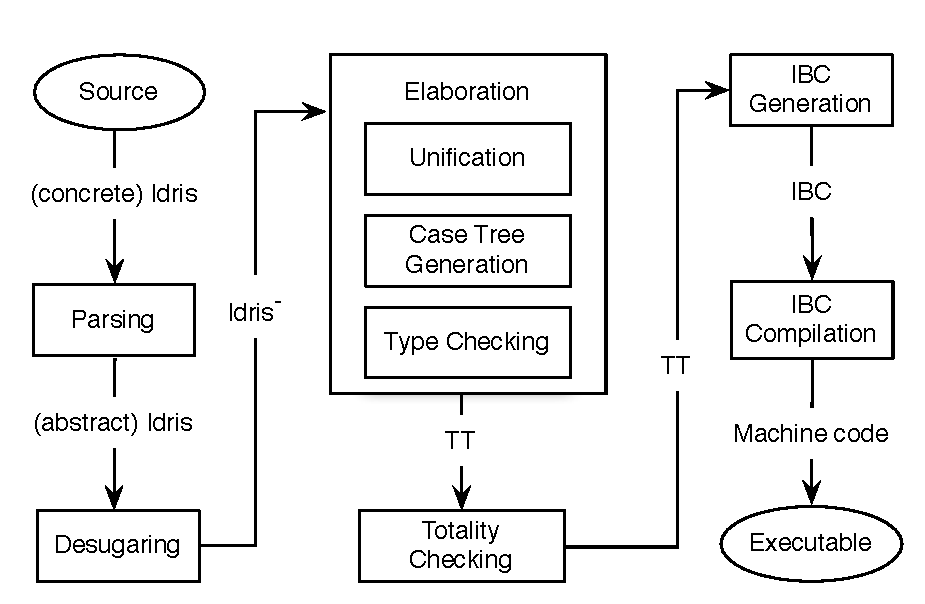
\includegraphics[scale=0.9]{figures/Idris-overview}
\caption{The phases of the Idris compiler. Phases are shown as rectangles, and
  each transition (arrow) is annotated with the input or output representation
  of a given phase. Ovals designate endpoints.}
\label{fig:idris-overview}
\end{figure}
An overview of the different phases of the Idris compiler is shown in
Figure~\ref{fig:idris-overview}. Starting with concrete Idris source code and
ending with a binary executable, each rectangle represents one phase of
compilation. During compilation, the input program is represented in several
different internal languages. Each arrow in Figure~\ref{fig:idris-overview}
is ascribed with the language in which the input program is represented when entering
or leaving a phase, respectively. Omitting a description of the machine code, these are:
\begin{itemize}
\item \textbf{(concrete) Idris}
The high-level language in which Idris programs are written.
\item \textbf{(abstract) Idris}
The abstract representation of the high-level Idris language generated by the parser.
\item \textbf{\IdrisM}
A (strict) subset of abstract Idris without any syntactic sugar. Do-notation and infix operators
are desugared, and implicit arguments are bound explicitly. Note that
\IdrisM{} and abstract Idris are essentially the same language, where the
syntactic sugar from abstract Idris is reduced to desugared terms in \IdrisM.
\item \textbf{TT}
The core type theory, TT, is a dependently typed lambda calculus with inductive
families and pattern matching. TT only allows pattern matching on top-level values,
so all \texttt{case}-expressions are converted to top-level pattern matching
during elaboration. In TT, all terms are fully annotated with their types and
all implicit arguments are explicit.
\item \textbf{Raw}
A (raw) representation of TT terms without any type information. This
representation is used for type reconstruction during type checking. As Raw is
internal to the type checking phase, it is not shown in
Figure~\ref{fig:idris-overview}, but has been included here for completeness and
later reference.
\item \textbf{IBC}
Idris Byte Code (IBC) is the bytecode representation of an Idris program.
\end{itemize}

Each of the language representations (except concrete Idris) are generated by a specific phase of
compilation, usually to reduce a complex representation to a simpler
representation which is easier to reason about and compile. Including the input
and output of the compiler, namely Source and Executable, the phases are:

\begin{itemize}
\item \textbf{Source}
The source code of the program, given in concrete Idris syntax.
\item \textbf{Parsing}
The parser generates an abstract syntax tree (abstract Idris) from the source code.
\item \textbf{Desugaring}
 In the desugaring phase, abstract Idris is reduced to \IdrisM{} by
 desugaring do-notation, implicit arguments, etc.
\item \textbf{Elaboration}
Elaboration reduces \IdrisM{} terms to terms in the core language, TT. The
elaboration phase consists of several notable sub-phases:
\begin{itemize}
\item \textit{Unification} Unification is the process of finding a substitution
  (also called a \texttt{unifier}) that identifies two terms. In Idris,
  unification enables elaboration to progress gradually by continual unification
  of holes with terms, until a complete TT term has been built. Also,
  unification is used for instantiation of implicit arguments. Further details
  will be provided in Section~\ref{sec:elaboration}.
\item \textit{Case Tree Generation}
A case tree\,\citep{Augustsson:1985} is generated for each function definition,
describing the structure of the top-level pattern matching on the left-hand side
of a definition. These case trees are
used for coverage checking by the totality checker.
\item \textit{Type Checking} All TT terms resulting from the previous steps of
  elaboration are type checked at the end of elaboration to ensure that no
  ill-typed terms are constructed. Type checking proceeds by mapping TT terms to
  Raw terms, and then reconstructing the type of each Raw term according to the
  typing environment. If the reconstructed type is convertible with the
  annotated type of the original TT term, type checking succeeds; otherwise, it
  fails. As the last stage of type checking, universe levels are checked by
  checking for cycles in a graph of universe constraints.
\item \textit{Totality Checking} During the totality checking phase, a totality
  analysis is performed on all function definitions. First, a coverage analysis
  determines whether the function in question is covering using the previously
  generated case trees. Next, a termination analysis based on the size-change
  principle is performed on functions with an inductive result type, while a
  productivity analysis is performed on functions with a coinductive result type via the
  syntactic guardedness principle.
\end{itemize}
\item \textbf{IBC Generation}
After successful elaboration, an Idris Byte Code representation is
generated by a script which is built up gradually during elaboration. 
\item \textbf{IBC Compilation}
During compilation, the IBC representation is reduced to machine code.
\item \textbf{Executable}
The final executable generated by the compiler.
\end{itemize}
%\subsection{Internal Representations}
%\subsection{High-Level Abstract Syntax}
%PDecl/PTerm
%	Top level abstract syntax
%	Functions with multiple clauses are multiple Decls

The most interesting parts of the compiler is the core type theory, TT, and the
elaboration phase, in which TT terms are built. These will now be explained in
greater detail. Also, a brief explanation of the implementation of coinductive
data types in Idris will be provided.

\section{TT, the Core Type Theory}
\label{sec:tt-core-type}
\todo{Write a description of how we write TT programs}
% increased confidence
% easier to compile, optimise and type check
%		TT
%			Dependently typed lambda calculus
%			Wrapped in case trees
%			Data and Type constructors??
TT is a dependently typed lambda calculus extended with top-level pattern
matching definitions and inductive families. It is deliberately kept small in order to provide increased
confidence in its correctness. A simple core type theory is also easier to
type check and optimise, and as will be shown in
Chapter~\ref{cha:infer-guard-recurs}, greatly simplifies the implementation of
our inference system for guarded recursion.
\begin{figure}[h]
\centering
\AxiomC{$\Gamma \vdash$ \underline{valid}}
\LeftLabel{Type}
\UnaryInfC{$\Gamma \vdash Type_n : Type_{n+1}$}
\DisplayProof

\vspace{1em}

\AxiomC{$\Gamma \vdash$ \underline{valid}}
\LeftLabel{Const$_1$}
\UnaryInfC{$\Gamma \vdash i : Int$}
\DisplayProof
\quad
\AxiomC{$\Gamma \vdash$ \underline{valid}}
\LeftLabel{Const$_2$}
\UnaryInfC{$\Gamma \vdash str : String$}
\DisplayProof

\vspace{1em}

\AxiomC{$\Gamma \vdash$ \underline{valid}}
\LeftLabel{Const$_3$}
\UnaryInfC{$\Gamma \vdash Int : Type_0$}
\DisplayProof
\quad
\AxiomC{$\Gamma \vdash$ \underline{valid}}
\LeftLabel{Const$_4$}
\UnaryInfC{$\Gamma \vdash String : Type_0$}
\DisplayProof

\vspace{1em}

\AxiomC{$(\lambda x:S) \in \Gamma$}
\LeftLabel{Var$_1$}
\UnaryInfC{$\Gamma \vdash x : S$}
\DisplayProof
\quad
\AxiomC{$(\forall x:S) \in \Gamma$}
\LeftLabel{Var$_2$}
\UnaryInfC{$\Gamma \vdash x : S$}
\DisplayProof
\quad
\AxiomC{$(\underline{let} \mapsto s:S) \in \Gamma$}
\LeftLabel{Val}
\UnaryInfC{$\Gamma \vdash x : S$}
\DisplayProof

\vspace{1em}

\AxiomC{$\Gamma \vdash f : (x : S) \to T$}
\AxiomC{$\Gamma \vdash s : S$}
\LeftLabel{App}
\BinaryInfC{$\Gamma \vdash f\ s : T[{s} / {x}]$}
\DisplayProof

\vspace{1em}

\AxiomC{$\Gamma; \lambda x : S \vdash e : T $}
\AxiomC{$\Gamma \vdash (x : S) \to T : Type_n$}
\LeftLabel{Lam}
\BinaryInfC{$\Gamma \vdash \lambda x : S . e : (x : S) \to T$}
\DisplayProof

\vspace{1em}

\AxiomC{$\Gamma; \forall x : S \vdash T : Type_m$}
\AxiomC{$\Gamma \vdash S : Type_n$}
\LeftLabel{Forall}
\RightLabel{$\exists p.m \leq p, n \leq p$}
\BinaryInfC{$\Gamma \vdash (s : S) \to T : Type_p$}
\DisplayProof

\vspace{1em}

\AxiomC{$\begin{matrix}
\Gamma \vdash e_1 : S
\\
\Gamma \vdash S : Type_n
\end{matrix}$}
\AxiomC{$\begin{matrix}
\Gamma; \underline{let} \x \mapsto e_1 : S \vdash e_2 : T
\\
\Gamma; \underline{let} \x \mapsto e_1 : S \vdash T : Type_n
\end{matrix}$}
\LeftLabel{Let}
\BinaryInfC{$\Gamma \vdash \underline{let}\ x \mapsto e_1 : S.\ e_2 : T[{e_1}/{x}]$}
\DisplayProof

\vspace{1em}

\AxiomC{$\Gamma \vdash x : A$}
\AxiomC{$\Gamma \vdash A' : Type_n$}
\AxiomC{$\Gamma \vdash A \preceq A'$}
\LeftLabel{Conv}
\TrinaryInfC{$\Gamma \vdash x : A'$}
\DisplayProof
\caption{The typing rules for the core type theory TT, borrowed from Brady\,\citep{BradyIdrisImpl13}.}
\label{fig:TT_typing_rules}
\end{figure}
The typing rules for TT are shown in Figure~\ref{fig:TT_typing_rules}. Most of these rules are standard, keeping in mind that types may
depend on values. In order to avoid Girard's paradox, i.e. that the type of
\texttt{Type} is \texttt{Type} (which is a logical inconsistency), a
cumulativity relation ($\preceq$) on universes is used, defined by the rules in
Figure~\ref{fig:TT_cumulativity_relation}.
\begin{figure}
\centering
\AxiomC{$\Gamma \vdash S \simeq T$}
\UnaryInfC{$\Gamma \vdash S \preceq T$}
\DisplayProof
\quad
\AxiomC{}
\UnaryInfC{$\Gamma \vdash Type_n \preceq Type_{n+1}$}
\DisplayProof

\vspace{1em}

\AxiomC{$\Gamma \vdash R \preceq S$}
\AxiomC{$\Gamma \vdash S \preceq T$}
\BinaryInfC{$\Gamma \vdash R \preceq T$}
\DisplayProof

\vspace{1em}

\AxiomC{$\Gamma \vdash S_1 \simeq S_2$} 
\AxiomC{$\Gamma; x : S_1 \vdash T_1 \preceq T_2$}
\BinaryInfC{$\Gamma \vdash \forall x:S_1.T_1 \preceq \forall x:S_2.T_2$}
\DisplayProof
\caption{The rules for the cumulativity relation.}
\label{fig:TT_cumulativity_relation}
\end{figure}
Notice that some of the rules for the cumulativity relation requires terms to be
convertible ($\simeq$), e.g. $S\simeq T$. Convertibility will be explained as
part of the type checking phase in Section~\ref{sec:type-checking}.

The rest of this report will contain both \texttt{TT} and Idris code
examples. Each block of code will be marked indicating what language it
contains. As some details of \texttt{TT} are not necessary to understand our
implementation, we use a different notation for \texttt{TT} than the one used by
Brady\,\citep{BradyIdrisImpl13}. Figure~\ref{fig:tt_notation} shows a \texttt{TT}-function
\texttt{vAdd} as written with first Brady's notation, followed by ours. Firstly,
we treat type class parameters as they are treated in high-level Idris (similar
to Haskell). Secondly we do not annotate the type of pattern variables. Not
shown in the example, we also do not annotate the type of lambda and
let-bindings. Furthermore, we use certain high-level Idris syntactic shorthands, such as
\texttt{[]} instead of \texttt{Nil}. Lastly, note that we use \texttt{=} rather than $\mapsto$.

\newcommand{\lstul}[1]{\ensuremath{\underline{\mbox{ #1}}}}

\begin{figure}[H]
\begin{lstlisting}[mathescape]
vAdd : ($a$ : Type) $\to$ ($n$ : Nat) $\to$ Num $a$ $\to$ 
         Vect $n$ $a$ $\to$ Vect $n$ $a$ $\to$ Vect $n$ $a$
$\lstul{var}$ $a$ : Type, $c$ : Type.
   vAdd $a$ Z $c$ (Nil $a$) (Nil $a$) $\mapsto$ Nil $a$
$\lstul{var}$ $a$ : Type, $k$ : Nat, $c$ : Type,
   $x$ : $a$, $xs$ : Vect $k$ $a$, $y$ : a, $ys$ : Vect $k$ $a$.
   vAdd $a$ (S $k$) $c$ ((::) $a$ $k$ $x$ $xs$)((::) $a$ $k$ $y$ $ys$)
         $\mapsto$ ((::) $a$ $k$ ((+) $c$ $x$ $y$) $xs$) (vAdd $a$ $k$ $c$ $xs$ $ys$)

vAdd : Num a $\Rightarrow$ (a : Type) $\to$ (n : Nat) $\to$ 
         Vect n a $\to$ Vect n a $\to$ Vect n a
vAdd a Z [] [] = []
vAdd a (S k) (x :: xs) (y :: ys)
      = (::) a k (x + y) (vAdd a k xs ys)
\end{lstlisting}  
  \caption{Edwin Brady's\,\citep{BradyIdrisImpl13} notation for \texttt{TT} compared to ours.}
  \label{fig:tt_notation}
\end{figure}

\section{Coinductive Data Types in Idris}
\label{sec:coind-data-types}
Idris supports inductive as well as coinductive type families. The latter is
modeled as lazily evaluated inductive families, where the types of all recursive
constructor arguments are tagged automatically with a special type constructor,
\texttt{Inf}. Values with an \texttt{Inf} type are possibly infinite, and thus
cannot be safely evaluated using a call-by-value strategy. In the vein of Abelson
and Sussman\,\citep{Abelson96SICP}, evaluation of such values is handled by two
special data constructors, \texttt{Delay} and \texttt{Force}. These provide
call-by-name evaluation, in the sense that all \texttt{Inf} values are initally
delayed, and then forced when needed. The compiler cannot always infer all possibly infinite arguments, e.g. when using mixed
induction-coinduction, so in these cases the user must manually tag the correct
argument types with \texttt{Inf}. Aside from the use of \texttt{Inf}, Idris also supports
lazy evaluation of inductively defined values.

\section{Elaboration}
\label{sec:elaboration}
The elaborator is similar to tactic-based theorem provers such as Coq\,\citep{Coq:manual},
which takes terms from \IdrisM{} to TT in a step-by-step manner. The idea is to
construct a TT term from a corresponding \IdrisM{} term by gradual refinement,
until a complete and well-typed TT term has been built. Before describing the
process of elaboration, the motivation behind the elaborator will be provided,
along with the intuitions underlying type checking and totality checking TT terms. 

\subsection{Motivation}
Instead of compiling \IdrisM{} directly to byte code, increased confidence in
the correctness of compilation can be obtained by first transforming a possibly
complex term in the high-level language to a simpler term in the core type
theory. This leads to a smaller trusted core, seeing as if we are
confident that TT can be correctly translated into byte code, and we can
show that any \IdrisM{} term can be correctly transformed
to a corresponding TT term, then we can be more confident in the correctness of
the high-level \IdrisM{} language than if it was translated directly to byte
code.

\subsection{Type Checking}
\label{sec:type-checking}
%Computing normal forms may require evaluation
%The type checker will not attempt to find normal forms for partial definitions.
% Type checking TT terms is a process with two high-level steps:

% \begin{enumerate}
% \item During elaboration, two forms of
% consistency checks are performed, namely type reconstruction and
% conversion checking.
% \item After the TT term resulting from elaboration has been fully built, the
%   definition is \emph{rechecked}.
% \end{enumerate}

% All type checking happens on TT terms. During elaboration, two forms of
% consistency checks are performed, namely type reconstruction and
% conversion checking. A common scenario is as follows:
% \begin{enumerate}
% \item Some tactic expects a term $e$ to have type $A$
% \item The type of $e$ is reconstructed with respect to a context $\Gamma$, such
%   that $e : B$
% \item A conversion check is performed on $A$ and $B$ with respect to $\Gamma$,
%   succeeding if $A$ is convertible with $B$, and failing otherwise.
% \end{enumerate}
% As an example we consider the tactic \textsc{Pi($\Gamma$, $n:S$, $?x:Type.x$)},
% which expects an $x$ of type $Type$, and is given an $n$ of type $S$. The type
% of $S$ is then reconstructed, such that $S : T$. If $T$ is convertible with
% $Type$, then $n$ is a well-typed argument, otherwise it is not.

In the elaboration phase, type checking plays a role both during and after the
construction of a TT term. Type checking a TT term $e$ against a type $T$ is a
twofold process, involving (1) type reconstruction and (2) conversion
checking. To determine whether $e : T$ holds, the type of $e$ is first
reconstructed as $S$, and then a conversion check between $S$ and $T$ is performed.

\subsubsection{Type Reconstruction}
To reconstruct the type of a TT term $e$, all type information is first erased from
the term using a forgetful mapping from TT to Raw, producing $e_{raw}$. The type of the $e_{raw}$ is
then reconstructed such that it conforms to the rules presented in
Figure~\ref{fig:TT_typing_rules}. All type information is available at this
point, so no type inference is performed (no new type information is
derived). Instead, type information is recovered from either the global context,
where the types of top-level definitions are stored, or the local context, where
the types of variables are stored.

\subsubsection{Conversion Checking}
Conversion checking happens by comparing the normal forms of two TT
terms. Finding these normal forms may require evaluation, since any of the two
terms can involve arbitrary expressions. Compile-time evaluation of TT terms is
defined by two contraction schemes, as explained by Brady\,\citep{BradyIdrisImpl13}.
When two TT terms $e_{1}$ and $e_{2}$ are convertible ($\simeq$), such that
$\Gamma\vdash e_{1} \simeq e_{2}$ holds, $e_{2}$ can be
obtained from $e_{1}$ by a finite number of applications of the contraction
schemes, where reversed applications are allowed.

% \paragraph{Aside: Rechecking} When a TT term is returned as the result of
% elaboration, the left-hand side and right-hand sides of a definition are
% \emph{rechecked} against each other using a conversion check, making sure that
% they still match. Rechecking ensures that an elaborated TT term is not only
% well-typed, but actually has the expected type. 

\subsection{Totality checking}
%		Happens during and after elaboration
%			What happens when and why?
%		Coverage: Case Trees
%		Termination: Size Change
%			When are the graphs build?
%		Productivity: Syntactic Guardedness
Totality checking is a prerequisite for type checking, since the conversion
checker will not attempt to find normal forms for definitions which have not
been proven total. In practice, this means that partial functions cannot be part
of a type declaration. The totality
checking procedure in Idris has three parts: coverage checking, totality
checking, and productivity checking.

The coverage checker analyzes the left-hand side pattern matching structure
using case trees\,\citep{Augustsson:1985}. These case trees are constructed from
TT terms by a special case tree elaborator, which in particular identifies
unmatched and default cases. If a definition is not covering, the totality
checker performs no further analysis.

The termination checker is a quite straightforward implementation of the
size-change termination principle\,\citep{LeeJones01SizeChange}. Since Idris
supports the definition of mutually recursive functions in a special block
designated by the keyword \texttt{mutual}, the termination checker
is invoked after the elaboration of each such block.

The productivity checker is an implementation of the principle of
syntactic guardedness\,\citep{Coquand94}. The current implementation is
part of the termination checker, since it merely checks that all
corecursive invocations happen under a special data constructor
``Delay'' (after normalization). The ``Delay'' constructor is used indicate lazy
evaluation, and is eliminated by its counterpart, ``Force''. After normalization,
a corecursive reference must therefore occur under under at least one
``Delay'' constructor in order to be productive.

\subsection{The Elaboration Process}
To enable construction of TT terms by gradual refinement, incomplete terms must
be supported by the elaboration process. Concretely, this happens by having
``holes'' (subgoals of incomplete terms) and ``guesses'' (possible
instantiations for a hole) as binders in the term language, inspired by
McBride's approach\,\citep{McBrideThesis:1999}. Elaboration happens within a
proof state, consisting of the (incomplete) proof term currently being
constructed, a queue of holes, a collection
of unsolved unification problems, and a typing context. At the head of the hole
queue is the hole which is currently being solved. Initially, the proof state
contains only one hole, but more holes can be added to and removed from the hole
queue as elaboration progresses.

As shown in Figure~\ref{fig:idris-overview}, elaboration is a quite complex
process where unification, case tree generation, and type checking are all
intertwined. The invocation of each of these phases is directed by tactics,
since the transformation of different terms requires them at different stages
during elaboration. Elaboration should therefore not be understood as a linear
process from unification to type checking, but rather as a process where each of
these phases are performed as needed.

In practice, elaboration proceeds within a monad \texttt{Elab}, which is
essentially a state monad which also offers error handling and additional
support for specific meta-operations on the state. These meta-operations are
applied to the proof state and the current proof term until all holes have been
resolved. According to Brady\,\citep{BradyIdrisImpl13}, four types of meta-operations are used:
\begin{itemize}
\item \textbf{Queries}, which are the tactics that do not modify the current
  proof term or the proof state. These include retrieving the current proof
  term, retrieving the type of a term, and retrieving the local context of a hole.
\item \textbf{Unification}, which solves unification problems relative to a context.
\item \textbf{Tactics}, which modify the current proof term and may modify the
  proof state in the process.
\item \textbf{Focusing}, which moves a hole to the head of the hole queue.
\end{itemize}
Due to their simplicity, we will forgo explanations of queries and
focusing, an instead elaborate further on unification and tactics.

\subsubsection{Unification}
The goal of unifying two terms $t_{1}$ and $t_{2}$ is to find a substitution
such that the two terms are convertible with respect to a given typing context,
$\Gamma$ (i.e. $\Gamma\vdash t_{1} \simeq t_{2}$). Hence, a unification problem
forms a triple ($\Gamma$, $t_{1}$, $t_{2}$). Unification of two terms may fail
if unification of subterms fail, or if solving one unification problem makes
related unification problems impossible to solve. Solving a unification problem
may lead to solutions of existing problems and introduce new problems.

Unification is used in throughout the elaboration process, for example for type checking
and for the gradual construction of TT terms. Also it is instrumental in the
process of inferring implicit arguments. Consider the implementation of a
\texttt{map} function on indexed lists (\texttt{Vect}) given in
Figure~\ref{fig:vect_map}. Here, \texttt{a}, \texttt{b}, and \texttt{n} are
implicit arguments which must be resolved. First, the implicit arguments are
made explicit through desugaring, as shown in
Figure~\ref{fig:vect_map_desugared}. The types of the implicit arguments cannot
be readily inferred, however, and must be solved by unification. Therefore, the
program in Figure~\ref{fig:vect_map_desugared} gives rise to the following
unification problems:
\begin{itemize}
\item ($\,\cdot\,$, \texttt{a : \_}, \texttt{a : Type})
\item ([a : Type], \texttt{b : \_}, \texttt{b : Type})
\item ([a : Type, b : Type], \texttt{n : \_}, \texttt{n : Nat})
\end{itemize}
The third part of each problem arise from the use of the names: The arguments
\texttt{a}, \texttt{b}, and \texttt{n} are used in positions where
\texttt{Type}, \texttt{Type}, and \texttt{Nat} are expected, respectively. To
solve each problem, the unification algorithm must be able to put a convertible
type at each binding site. In this case, the solutions are all straightforward,
and the resulting program is shown in Figure~\ref{fig:vect_map_resolved}. The
important thing to note is that all of these problems have a unique solution,
making unambiguous inference possible.

\begin{figure}
\begin{lstlisting}[mathescape]
map : (a $\to$ b) $\to$ Vect n a $\to$ Vect n b
map f (x :: xs) = f x :: map f xs
\end{lstlisting}
  \caption{A map function for an indexed list type \texttt{Vect}.}
  \label{fig:vect_map}
\end{figure}

\begin{figure}
\begin{lstlisting}[mathescape]
map : (a : _) $\to$ (b : _) $\to$ (n : _) $\to$ 
      (a $\to$ b) $\to$ Vect n a $\to$ Vect n b
map _ _ _ f (x :: xs) = 
                    ((::) _ _ (f _ _ x) (map _ _ _ f xs))
\end{lstlisting}
  \caption{A desugared map function for a type \texttt{Vect} with implicit
    arguments made explicit.}
  \label{fig:vect_map_desugared}
\end{figure}

\begin{figure}
\begin{lstlisting}[mathescape]
map : (a : Type) $\to$ (b : Type) $\to$ (n : Nat) $\to$ 
      (a $\to$ b) $\to$ Vect n a $\to$ Vect n b
map a b n f (x :: xs) = ((::) n b (f a b x) (map a b n f xs))
\end{lstlisting}
  \caption{A desugared map function for a type \texttt{Vect} with resolved
    implicit arguments.}
  \label{fig:vect_map_resolved}
\end{figure}

\subsubsection{Tactics}
Although unification is an important part of elaboration, the core of the
elaborator is tactics. Tactics modify the current proof term, each describing a
possible step in the transformation of a term from \IdrisM{} to TT. 

%The following are a subset of the tactics which may be part of such a transformation: 

% \begin{itemize}
% \item \textsc{Lambda($\Gamma$, $n$, $?x:T.x$)} creates a lambda binding with
%   respect to a context $\Gamma$ with name $n$, from a proof term which
%   expects a binder ($?x:T.x$).
% \item \textsc{Pi($\Gamma$, $n:S$, $?x:Type.x$)} creates a pi-binding (dependent
%   product type) with name $n$ with respect to a context $\Gamma$, from a
%   proof term which expects a type binder.type checking
% \item \textsc{Let($\Gamma$, $(n:S) \mapsto v$, $?x:T.x$)} creates a let-binding
%   mapping $n$ to $v$ with respect to a context $\Gamma$ from a
%   proof term which expects a binder.
% \item \textsc{Subst($x$, $e$)} which instantiates a hole $x$ with a term
%   $e$, often as a result of unification.
% \item \textsc{PrimUnify($\Gamma$, $e_{1}$, $e_{2}$)} which attempts to unify terms
%   $e_{1}$ and $e_{2}$ with respect to a context $\Gamma$. 
% \item \textsc{Check($\Gamma$, $e$)} which type checks a term $e$ with
%   respect to a context $\Gamma$, returning the type of $e$.
% \item \textsc{Convert($\Gamma$, $e_{1}$, $e_{2}$)} which checks that the
%   cumulativity relation holds between $e_{1}$ and $e_{2}$ by performing a
%   conversion with respect to a context $\Gamma$. 
% \item \textsc{Normalise($\Gamma$, $e$)} which returns the normal form of a term
%   $e$ with respect to a context $\Gamma$.
% \end{itemize}

Tactics describe both concrete operations on the proof term, such as binder
creation, meta-operations on the proof state, such as hole substitution, and
meta-operations ensuring consistency, such as type checking. Complex
operations which require evaluation, e.g. \textsc{Check} and \textsc{Convert},
may invoke operations which are external to the tactic system, such as type
checking.

\subsection{Delaboration}
Mainly to support error reporting, a \emph{de}laborator is also a part of the
compiler. The delaborator builds an \IdrisM{} term from a TT term, striving to
build a term which resembles the user-written term as closely as
possible. However, the delaboration process is not always able to correctly
reconstruct the user-written program, and should therefore not be relied upon
for program analysis.

\section{A Short Recapitulation}
%\todo{Er lidt usikker på denne afslutning, men ellers slutter det næsten for
%brat?}
From the Idris input provided by the user, an abstract syntax tree in abstract
Idris is created. Through desugaring of do-notation and implicit arguments, an
\IdrisM{} representation is built. Elaboration builds a TT term from an
\IdrisM{} term by constructing a proof of a transformation from \IdrisM{} to
TT. This proof is provided as a series of tactics operating on a proof state,
each of which may require unification and type checking. Unification is used for
type checking, term construction, and inference of implicit arguments. Type
checking ensures consistency through type reconstruction and conversion
checks. After elaboration, the totality checker provides the guarantees
necessary for avoiding the reduction of partial definitions during following
invocations of the type checker. During elaboration, a script is accumulated
which describes the resulting IBC file. After the previous phases have been
completed, an IBC file is written, and from this, machine code is generated.

%incomplete terms must be supported by the elaboration process. 


%########
%% TT
% Alt er eksplicit
% Typeregler

%%% Type checking

%% Idris- / Desugaring
% Desugaring er en transformation fra Idris- til Idris-

%% Elaboration
% Hvorfor elaboration?
% Faser "smelter sammen" 
% Teknisk forklaring (tactic prover)

%% Totality checking
% Size-change termination
% Nuværende implementation af produktivitetschecker
% Totality er en forudsætning for type checking
% Erasure? (måske)


%########

%%% Local Variables:
%%% mode: latex
%%% TeX-master: "../copatterns-thesis"
%%% End:


\chapter{Coinductive Records in Idris}
\label{cha:coind-records-idris}
We have previously discussed the concept of data with a top-level product
structure. In this chapter we discuss how we have modified the current
implementation of the records in Idris to focus on observations rather
than constructions.

\section{Intuition}
To understand our implementation, let us first look at the current
implementation of records in Idris. In Figure~\ref{fig:records_in_idris} an
example of a product type, here a \texttt{Pair}, is defined as a
record. Syntactically, this looks a lot like a data declaration, except for the
\texttt{record} keyword. Also, we are required to define exactly one
constructor, unlike data declarations, where we can have zero or many.

\begin{figure}[h]
\begin{lstlisting}
record Pair : Type -> Type -> Type where
  MkPair : (fst : a) -> (snd : b) -> Pair a b
\end{lstlisting}
  \caption{Current record syntax in Idris.}
  \label{fig:records_in_idris}
\end{figure}

The difference between a record and a data declaration does not appear until just
before elaboration. Here the record is elaborated as a data declaration
(literally Figure~\ref{fig:records_in_idris}, with the keyword \texttt{data}
instead of \texttt{record}), with a set of functions generated. Both a
\emph{projection} and an \emph{update} function is generated for each named
parameter in the constructor, in the \texttt{Pair} example \texttt{fst} and
\texttt{snd}. These projection functions are then placed in a namespace with the
name of the type, in this case \texttt{Pair}. 

\begin{figure}[h]
\begin{lstlisting}
data Pair : Type -> Type -> Type where
  MkPair : (fst : a) -> (snd : b) -> Pair a b

namespace Pair
  fst : Pair a b -> a
  fst (MkPair x _) = x

  snd : Pair a b -> b
  snd (MkPair _ y) = y

  set_fst : Pair a b -> a -> Pair a b
  set_fst (MkPair _ y) x = MkPair x y

  set_snd : Pair a b -> b -> Pair a b
  set_snd (MkPair x _) y = MkPair x y
\end{lstlisting}
  \caption{\texttt{Pair} from Figure~\ref{fig:records_in_idris} desugared. Note
    that this is a slightly prettified version.}
  \label{fig:pair_desugared}
\end{figure}

An example of how records are desugared can be seen in
Figure~\ref{fig:pair_desugared}. This means that records are a high-level feature, syntactic sugar, and
as such so should our implementation of them be.

\subsection{Corecords}
Just as records are desugared to data declarations, corecords should be
desugared to codata declarations. From the parser, the difference between data and
codata declarations is a flag given to the elaborator. We can apply the same
approach to corecords, with a flag denoting whether the declaration should be
desugared to a data or codata declaration. 

\section{Implementation}
Our implementation is a syntactic desugared. In the following we will describe
how each component of the new syntax translates to what in a desugared
version. So without further ado, we present the following record syntax: 

\begin{lstlisting}[mathescape]
record <name> <parameters> where
  <field$_1$ name> : <field$_1$ type>
  <field$_2$ name> : <field$_2$ type>
  ...
  <field$_n$ name> : <field$_n$ type>
  constructor <constructor name> <field or parameter names>
\end{lstlisting}

\paragraph{Parameters}
The parameters desugar to the type constructor. A parameter can be either (1) a
name binded to a type, e.g. \texttt{(name : Type)} or (2) a free name,
e.g. \texttt{a}. If just a free name is given it is assumed to be of type
\texttt{Type}. As such writing \texttt{a} is interpreted as \texttt{(a : Type)}

Be default, the parameters are given as explicit parameters to the type
constructor and implicit parameters to the data constructor. Both of these
defaults can be overridden. A parameter can be marked as implicit by
surrounding it with curly braces, replacing any existing parentheses. How we
stop parameters from being implicit to the data constructor will be discussed later.

\paragraph{Fields}
The fields defined by a list of names and types separated by a \texttt{:}. All
fields will, again by default, be explicit arguments to the data
constructor. Similar to the original Idris-record implementation, projection and
update functions are generated for each field.
\paragraph{Data Constructor}
The line starting with the \texttt{constructor} keyword is an, optional,
customizing of the data constructor. This allows the user to define a name for
the constructor if desired, but it can also be omitted in which case a name
based on the type, avoiding name clashes, will be created during elaboration.

The last part, \texttt{field names}, is again optional. The programmer can list
the parameters and fields in order to change how they behave in the generated
data constructor. Here, a name on its own will be forced to be explicit, and a
name surrounded by curly braces will be forced implicit. Names can be omitted,
leaving them untouched.

In the end all of this will be desugared to a data declaration with a
constructor from the parameters and fields to a record value.

\begin{figure}[h]
\begin{lstlisting}
record Pair a b where
  fst : a
  snd : b

record Foo (param : Nat) where
  num : Int
  constructor ConsFoo param

corecord Stream a where
  head : a
  tail : Stream a
  constructor (::)
\end{lstlisting}
  \caption{Record examples.}
  \label{fig:new_record_examples}
\end{figure}

\begin{figure}[h]
\begin{lstlisting}
data Pair : Type -> Type -> Type where
  MkPair : (fst : a) -> (snd : b) -> Pair a b

data Foo : (param : Nat) -> Type where
  ConsFoo : (param : Nat) -> (num : Int) -> Foo param

codata Stream a where
  (::) : (head : a) -> (tail : Stream a) -> Stream a
\end{lstlisting}
  \caption{The (co)data declaration resulting from desugaring the (co)record
    declarations from Figure~\ref{fig:new_record_examples}}
  \label{fig:new_record_examples_desugared}
\end{figure}

In Figure~\ref{fig:new_record_examples} a few examples of the above described
syntax can be seen, and Figure~\ref{fig:new_record_examples_desugared} depicts how
they desugar. For the sake of simplicity only the desugared data and codata
declarations are shown. More desugaring examples can be found in
Appendix~\ref{cha:record-examples}.

Note that at the time of writing, while almost done, this is not yet fully
implemented.

%%% Local Variables:
%%% mode: latex
%%% TeX-master: "../copatterns-thesis"
%%% End:


%!TEX root = ../copatterns-thesis.tex
\chapter{Adding Copatterns}
\label{sec:adding_copatterns}
Copatterns can be added to Idris without changing its core, the TT
calculus. Throughout this chapter, we will show how copatterns can be implemented as
syntactic sugar, i.e. a transformation from \IdrisM{} to \IdrisM{}, such that
all copattern clauses have been reduced to pattern clauses by the
time elaboration is reached.

% What, Why
\section{Intuition}
%#########
% Eliminationsregler => Introduktionsregler
% Top-level produktstruktur (een introduktionsregel)
% Pattern matching?
%#########
Following the discussion in Section~\ref{sec:prod-vs.-copr}, support for
copatterns have only been added for record types, both inductive and
coinductive. This decision is based upon the fact that Idris record types have
an obvious top-level structure, making them ideal companions for
copatterns. All examples are therefore given for record types only.

\subsection{The Duality Between Construction and Observation}
\label{sec:dual-betw-constr}
Desugaring copattern clauses, which give definitions by observation, to pattern
clauses, which give definitions by construction, relies on the duality between
introduction and elimination rules for (co)inductive types. For our first example,
we will consider the simple record type \texttt{Pair} in
Figure~\ref{fig:record_pair}. 
\begin{figure}
\begin{lstlisting}[mathescape]
record Pair (a : Type) (b : Type) where
  MkPair : (fst : a) $\to$ (snd : b) $\to$ Pair a b
\end{lstlisting}
  \centering
  $\begin{matrix} 
    \frac { \Gamma \,\vdash\, x\,:\,a \quad \Gamma \,\vdash\, y\,:\,b }{
      \Gamma\, \vdash\,MkPair\,x\,y\,:\,Pair\,a\,b} \scriptstyle I_{Pair}
  & \frac { \Gamma \,\vdash\, e\,:\,Pair\, a\,b }{ \Gamma\,
    \vdash\,fst(e)\,:\,a} \scriptstyle E_{fst}
  & \frac { \Gamma\, \vdash\, e\,:\,Pair\, a\,b }{ \Gamma\, \vdash\,
    snd(e)\,:\,b } \scriptstyle E_{snd}  \end{matrix}$
  $\vspace{12pt}$
  $\begin{matrix}
      \frac { \Gamma\, \vdash\, MkPair\,x\,y\,:\,Pair\,a\,b }{ \Gamma
      \,\vdash\, fst(MkPair\,x\,y)\,\equiv\,x  } \eta_{fst}  & \frac { \Gamma\, \vdash\,
      MkPair\,x\,y\,:\,Pair\,a\,b }{ \Gamma\, \vdash \,snd(MkPair\,x\,y)\,\equiv\,y } \eta_{snd} \end{matrix}$
  \caption{A record defining a type \texttt{Pair}, along with its introduction,
    elimination, and $\eta$-rules.}
  \label{fig:record_pair}
\end{figure}
The traditional way of creating a value of type \texttt{Pair} is by construction
using pattern clauses, as shown in Figure~\ref{fig:pair_example_pattern}. Here,
we construct a value of \texttt{Pair} using its introduction rule, giving the values
\texttt{``Idris''} and \texttt{42} as arguments. We can observe the data in the
constructed value by using the elimination rules \texttt{fst} and \texttt{snd},
which have corresponding $\eta$-rules as expected (see
Figure~\ref{fig:record_pair}). As seen from
Figure~\ref{fig:pair_example_pattern_typing_derivation}, such observations
provide unsurprising results.
\begin{figure}
\begin{lstlisting}
pattern : Pair String Nat
pattern = MkPair "Idris" 42
\end{lstlisting}
  \caption{A value of \texttt{Pair} defined by construction.}
  \label{fig:pair_example_pattern}
\end{figure}

\begin{figure}
\centering
    $
     \frac { \Gamma \,\vdash\, "Idris"\,:\,String \quad \Gamma \,\vdash\, 42\,:\,Nat }{
      \Gamma\, \vdash\,MkPair\,"Idris"\,42\,:\,Pair\,String\,Nat} \scriptstyle
    I_{Pair}$
   $\vspace{10pt}$
  $\begin{matrix} \frac { \Gamma \,\vdash\,MkPair\,"Idris"\,42\,:\,Pair\, String\,Nat }{ \Gamma\,
    \vdash\,fst(MkPair\,"Idris"\,42)\,:\,String} \scriptstyle E_{fst}
  & \frac { \Gamma\, \vdash\,MkPair\,"Idris"\,42\,:\,Pair\,String\,Nat }{ \Gamma\, \vdash\,
    snd(MkPair\,"Idris"\,42)\,:\,Nat } \scriptstyle E_{snd}  \end{matrix}$
   $\vspace{10pt}$
  $\begin{matrix}
      \frac { \Gamma\, \vdash\, MkPair\,"Idris"\,42\,:\,Pair\,String\,Nat }{ \Gamma
      \,\vdash\, fst(MkPair\,"Idris"\,42)\,\equiv\,"Idris"  } \eta_{fst}  & \frac { \Gamma\, \vdash\,
      MkPair\,"Idris"\,42\,:\,Pair\,String\,Nat }{ \Gamma\, \vdash \,snd(MkPair\,"Idris"\,42)\,\equiv\,42 } \eta_{snd} \end{matrix}$
  \caption{Using the rules for \texttt{Pair} on the example in Figure~\ref{fig:pair_example_pattern}.}
  \label{fig:pair_example_pattern_typing_derivation}
\end{figure}

The idea behind copatterns is that we can treat the (co)data constructor as a
black box (\texttt{MkPair} in above example),
defining only the values we expect to observe when making specific observations
on the constructed (co)data. As an example,
Figure~\ref{fig:pair_example_copatterns} shows how we can use copatterns to
define a program by observation which is equivalent to the definition by
construction in Figure~\ref{fig:pair_example_pattern}. The most striking
difference is that \texttt{pattern$^\prime$} itself is never explicitly
defined. Instead, it is defined implicitly by the two copattern clauses, which
provide all the data necessary to derive a corresponding pattern clause, as in Figure~\ref{fig:pair_example_pattern}. From
this observation, we arrive at the main intuition behind our desugaring
procedure: Any definition given by copattern clauses has an equivalent
definition given by pattern clauses, and this definition can be derived without
providing any further information. To make this intuition concrete, consider the
derivation in
Figure~\ref{fig:pair_elimination_on_introduction_rules_rewrite}. Rewriting with
the reduction rules defined in Figure~\ref{fig:pair_example_copatterns}, the
elimination rules for \texttt{Pair} are used to directly derive the right-hand
side of the \texttt{pattern} example from
Figure~\ref{fig:pair_example_pattern}. 

\begin{figure}
\begin{lstlisting}[mathescape]
pattern$^\prime$ : Pair String Nat
fst pattern$^\prime$ = "Idris"
snd pattern$^\prime$ = 42
\end{lstlisting}
  \caption{A value of \texttt{Pair} defined by construction.}
  \label{fig:pair_example_copatterns}
\end{figure}

\begin{figure}
  \centering
$\frac { \begin{matrix} \frac { \Gamma \, \vdash \,pattern'\, :\,
      Pair\, String\, Nat }{ \Gamma \, \vdash \, "Idris"\,:\,String
    } \scriptstyle E_{fst}   & \frac { \Gamma \, \vdash \,pattern'\, :\, Pair\, String\,
      Nat }{ \Gamma \, \vdash \, 42\,:\,Nat } \scriptstyle E_{snd}  \end{matrix} }{
  \Gamma \, \vdash \, MkPair\, "Idris"\, 42\, :\, Pair\, String\, Nat } \scriptstyle I_{ Pair }$
  \caption{Deriving the right-hand side of \texttt{pattern} from \texttt{pattern'}.}
  \label{fig:pair_elimination_on_introduction_rules_rewrite}
\end{figure}

\subsection{Desugaring Copatterns}
While the derivation in
Figure~\ref{fig:pair_elimination_on_introduction_rules_rewrite} provides a fine
display of our intention, such a direct derivation is only possible for simple
examples which have only one resulting pattern clause. In particular, desugaring
copatterns becomes more complex as the following challenges must be taken into account:

\begin{enumerate}
\item Nested copatterns
\item Pattern matching
\item Subsumed copattern clauses
\item Non-covering definitions
\end{enumerate}

To address each of these challenges, we have devised a desugaring procedure for
copatterns which operates in three steps:

\begin{enumerate}
\item \textbf{Expansion}, in which right-hand sides are expanded into partially
  defined constructor invocations.
\item \textbf{Reduction}, in which copatterns are eliminated from the reduction rules.
\item \textbf{Merging}, in which compatible clauses are merged into one clause.
  \begin{enumerate}
  \item Identify compatible clauses
  \item Merge compatible clauses
  \end{enumerate}
\end{enumerate}

Before discussing how our solution tackles each of the challenges, the inner
workings of the procedure will be illustrated with a simple example. Consider
the program \texttt{zeros} in Figure~\ref{fig:zeros}, which produces a value of
the type \texttt{Stream} defined in Figure~\ref{fig:corecord_stream}. In the
first step of desugaring \texttt{zeros}, expansion, the right-hand side of each
copattern clause is expanded into an explicit projection on a partially defined
Stream. Thus, the \texttt{head} clause of Figure~\ref{fig:desugared_zeros_step1}
may be read as: ``The \texttt{head} of \texttt{zeros} is the \texttt{head} of
the partially defined \texttt{Stream} which has \texttt{Z} as its first
constructor argument''. A corresponding reading exists for the \texttt{tail}
clause. \IdrisM{} metavariables are inserted for constructor arguments where
output has yet to be defined, e.g. \texttt{?zeroshead}.

\begin{figure}
\begin{lstlisting}[mathescape]
corecord Stream (a : Type) where
  head : a
  tail : Stream a
  constructor (::)
\end{lstlisting}
  \centering
  $\begin{matrix} 
    \frac { \Gamma \,\vdash\, x\,:\,a \quad \Gamma \,\vdash\, xs\,:\,Stream\,a }{
      \Gamma\, \vdash\,(x\,::\,xs)\,:\,Stream \,a} \scriptstyle I_{Stream}
  & \frac { \Gamma \,\vdash\, s\,:\,Stream\, a }{ \Gamma\,
    \vdash\,head(s)\,:\,a} \scriptstyle E_{head}
  & \frac { \Gamma\, \vdash\, s\,:\,Stream\, a }{ \Gamma\, \vdash\,
    tail(s)\,:\,Stream\, a } \scriptstyle E_{tail}  \end{matrix}$
  $\vspace{10pt}$
  $\begin{matrix}
      \frac { \Gamma\, \vdash\, (x\,::\,xs\,:\,Stream\,a }{ \Gamma
      \,\vdash\, head(x\,::\,xs)\,\equiv\,x  } \eta_{head}  & \frac { \Gamma\, \vdash\,
      (x\,::\,xs)\,:\,Stream\,a }{ \Gamma\, \vdash \,tail(x\,::\,xs)\,\equiv\,xs } \eta_{tail} \end{matrix}$
  \caption{A coinductive record type \texttt{Stream} defining an infinite list,
    along with introduction, elimination, and $\eta$-rules.}
  \label{fig:corecord_stream}
\end{figure}

\begin{figure}
\begin{lstlisting}[mathescape]
zeros : Stream Nat
head zeros = Z
tail zeros = zeros
\end{lstlisting}
  \caption{A function \texttt{zeros} defining a stream of 0.}
  \label{fig:zeros}
\end{figure}

In the second step, reduction, each clause from
Figure~\ref{fig:desugared_zeros_step1} is reduced by removing equivalent
projections on both side of a clause, similar to how one would reduce a
mathematical equation. The result of the reduction is shown in
Figure~\ref{fig:desugared_zeros_step2}. We are allowed to perform such
reductions at this point because all the clauses make right-hand side
projections directly on the (as yet unmerged) output of the function, while all
the left-hand side projections happen directly on the input.

\begin{figure}
\begin{lstlisting}[mathescape]
zeros : Stream Nat
head zeros = head (Z :: ?zerostail)
tail zeros = tail (?zeroshead :: zeros)
\end{lstlisting}
  \caption{Desugaring \texttt{zeros}, step 1: Expansion.}
  \label{fig:desugared_zeros_step1}
\end{figure}

\begin{figure}
\begin{lstlisting}[mathescape]
zeros : Stream Nat
-- Before: head zeros = head (Z :: ?zerostail)
-- Eliminate 'head' on each side
zeros = Z :: ?zerostail
-- Before: tail zeros = tail (?zeroshead :: zeros)
-- Eliminate 'tail' on each side
zeros = ?zeroshead :: zeros
\end{lstlisting}
  \caption{Desugaring \texttt{zeros}, step 2: Reduction.}
  \label{fig:desugared_zeros_step2}
\end{figure}

The final step, merging, is actually a two-step process, where compatible clauses are
merged with each other such that their right-hand sides are combined into
possibly complete constructor invocations. Some of the right-hand sides may remain
incomplete after the merging step if the definition we are desugaring is not
covering. In Figure~\ref{fig:desugared_zeros_step3a}, the clauses of
\texttt{zeros} which are compatible with each other are identified. Since
\texttt{zeros} is a simple example, the two clauses are compatible with each
other because their left-hand sides are identical. The clauses are
therefore merged into one clause, as shown in Figure~\ref{fig:desugared_zeros_step3b}.

\begin{figure}
\begin{lstlisting}[mathescape]
zeros : Stream Nat
-- The two clauses are compatible with each other
(1) zeros = Z :: ?zerostail
(2) zeros = ?zeroshead :: zeros
\end{lstlisting}
  \caption{Desugaring \texttt{zeros}, step 3a: Identifying compatible
    clauses. The clauses have been numbered for reference.}
  \label{fig:desugared_zeros_step3a}
\end{figure}

\begin{figure}
\begin{lstlisting}[mathescape]
zeros : Stream Nat
(1,2) zeros = Z :: zeros 
\end{lstlisting}
  \caption{Desugaring \texttt{zeros}, step 3b: Merging compatible clauses. The
    numbers indicate that both of the clauses from
    Figure~\ref{fig:desugared_zeros_step3a} have been merged into one clause.}
  \label{fig:desugared_zeros_step3b}
\end{figure}

\begin{definition}[\textit{Compatibility}]
\label{def:compatibility}
  Compatibility is a reflexive, transitive, and anti-symmetric binary relation
  $C$ on pattern clauses which describes whether the pattern in one pattern
  clause is more general or equally general to the pattern in another pattern
  clause. Let $V$ be a function which, given an argument pattern, returns the set of
  values matched by that pattern. For two pattern clauses
  $a\,p_{1}\,p_{2}\,\cdots\,p_{n}\,=\,rhs_{a}$ and
  $b\,q_{1}\,q_{2}\,\cdots\,q_{n}\,=\,rhs_{b}$ of an $n$-ary function,
  $(a,b)\in C$ if $V(p_{i})\subseteq V(q_{i})$ for $0 < i\le n$. For a nullary
  function, all pattern clauses are trivially compatible.
\end{definition}
% if the set of values
% for each argument $i$ matched by the pattern of $a$, $P_{i}(a)$, is a subset of of the set of
% values for each argument $i$ matched by the pattern of $b$, $P_{i}(b)$ i.e.
% $P_{i}(a)\subseteq P_{i}(b)$ for all $0 < i\le n$. 

\subsubsection{Addressing the Challenges}
The three-step desugaring procedure presented above has been devised as a
unified solution to four main challenges that arise when desugaring is performed
as a transformation from \IdrisM{} to \IdrisM{}. As we go through each of the
challenges, the \texttt{dupNth} program in Figure~\ref{fig:dupNth} will serve as
a running example of the desugaring of a non-trivial definition with copattern
clauses.

\paragraph{Challenge 1: Nested Copatterns}
Copatterns, i.e. left-hand side projections, can be nested arbitrarily as long
as the nesting is well-typed. As described in
Chapter~\ref{cha:coind-records-idris}, definitions with copatterns only behave
as intended when all projection names are unique. Therefore, our solution
assumes that projection names not only indicate semantics, but also argument
positions to the corresponding constructor. To illustrate, consider the
transformation of clause (2) from Figure~\ref{fig:dupNth} to the expanded clause
\texttt{(2)} in Figure~\ref{fig:desugared_dupNth_step1}. Because this clause
defines the \texttt{head} of the \texttt{tail} of the output, the expanded
clause has the right-hand side, \texttt{head~s}, inserted at this position in
the partially defined constructor on the right-hand side of (2) in
Figure~\ref{fig:desugared_dupNth_step1}. The same reasoning holds for the remaining clauses.

In general, nested copatterns are handled in the first two steps, expansion and
reduction. Expansion ensures that the original right-hand sides are inserted
into the correct positions in the expanded constructor invocations, while
reduction eliminates all left-hand side projections through equational
reasoning. A different solution to the problem of handling nested copatterns has
been proposed by Setzer et al.\,\citep{Setzer14Unnesting}, in which auxiliary
functions are created for each level of nested copatterns. This approach will be
described for an alternative solution in Section~\ref{sec:copatterns-implementation-discussion}.

\paragraph{Challenge 2: Pattern Matching}
Whenever the copattern clauses for a definition have different patterns on the
left-hand side, these patterns must be preserved in the desugared version of the
definition. After eliminating copatterns in the reduction step
(Figure~\ref{fig:desugared_dupNth_step2}), preservation of pattern matching is
ensured in the first sub-step of merging
(Figure~\ref{fig:desugared_dupNth_step3a}), where compatible clauses are
identified. In the following sub-step (Figure~\ref{fig:desugared_dupNth_step3b}), only compatible clauses are
merged. Merging only compatible clauses ensures that a clause is only merged
with other clauses which match the same or a more general set of input values. As an example, we will show exactly why clause (2) is compatible
with clause (1) as postulated in
Figure~\ref{fig:desugared_dupNth_step3a}. The proof
proceeds in Figure~\ref{fig:compatibility_proof}. Note that if, in Figure~\ref{fig:compatibility_proof}, $m_{1}$ had been
$S\,m_{1}$ instead, $(2,1)\notin C$ since $V(S\,m_{1}) =
\{\,x\,|\,x\,:\,Nat\,\setminus\{Z\}\}$, and $V(Z)\not\subseteq V(S\,m_{1})$.

\begin{figure}
From
Definition~\ref{def:compatibility}, we must show: $(2,1)\in C$, where (2) and (1) are clauses from
Figure~\ref{fig:desugared_dupNth_step3a}.
\\\\
We consider the left-hand sides of (2) and (1), respectively:\\
$lhs_{(2)} = dupNth\,s_{(2)}\,n_{(2)}\,Z$\\
$lhs_{(1)} = dupNth\,s_{(1)}\,n_{(1)}\,m_{(1)}$\\
\\
For each sub-pattern, we define the set of matching values:\\
$V(s_{2}) = \{\,x\,|\,x\,:\,Stream\,a\}$\\
$V(n_{2}) = \{\,x\,|\,x\,:\,Nat\}$\\
$V(Z) = \{Z\}$\\
$V(s_{1}) = \{\,x\,|\,x\,:\,Stream\,a\}$\\
$V(n_{1}) = \{\,x\,|\,x\,:\,Nat\}$\\
$V(m_{1}) = \{\,x\,|\,x\,:\,Nat\}$\\
\\
Having defined these, the following must hold:
\\
$V(s_{2})\subseteq V(s_{1}) = \{\,x\,|\,x\,:\,Stream\,a\}\subseteq\,\{\,x\,|\,x\,:\,Stream\,a\}\,\qed$\\
$V(n_{2})\subseteq V(n_{1}) =
\{\,x\,|\,x\,:\,Nat\}\subseteq\,\{\,x\,|\,x\,:\,Nat\}\,\qed$\\
$V(Z)\subseteq V(m_{1}) = \{Z\}\subseteq\,\{\,x\,|\,x\,:\,Nat\}\,\qed$\\\\
Consequently, $(2,1)\in C$
  \caption{From Figure~\ref{fig:desugared_dupNth_step3a}, clause (2) is
    compatible with clause (1).}
  \label{fig:compatibility_proof}
\end{figure}


\paragraph{Challenge 3: Subsumed Copattern Clauses}
In addressing Challenge 2, we stated that different left-hand side patterns must
be preserved in the output. Nevertheless, the pattern from clause (1) in
Figure~\ref{fig:desugared_dupNth_step3a} does not occur in the
desugared version of the function in
Figure~\ref{fig:desugared_dupNth_step3b}. Due to the fact that clause (1) is
more general than all the other clauses, it is subsumed by these in the final
output, such that the right-hand side of (1) is a part of the right-hand side of
both the desugared clauses. The set of subsumed copattern clauses for a
definition are exactly the clauses which are compatible with all other clauses.  

\paragraph{Challenge 4: Non-covering Defintions} As Idris allows users to
define functions which are not covering (see
Definition~\ref{def:covering_function}), partial definitions with copatterns
should be possible as well. With our desugaring procedure, the solution to this
challenge is provided ``for free'', since the metavariables which are inserted
during the expansion phase are simply not replaced with any proper definition if
none is given. A non-covering version of the \texttt{dupNth} function is shown
in Figure~\ref{fig:dupNth_partial}, along with its desugared version.

\begin{figure}
\begin{lstlisting}[mathescape]
||| Duplicate every nth element of s, 
||| starting with the mth element.
||| @s the stream
||| @n how often
||| @m where to start
dupNth : Stream a $\to$ Nat $\to$ Nat $\to$ Stream a
(1) head       (dupNth s n m)       = head s
(2) head (tail (dupNth s n Z))      = head s
(3) head (tail (dupNth s n (S m'))) = head (tail s)
(4) tail (tail (dupNth s n Z))      = tail (dupNth s n n)
(5) tail (tail (dupNth s n (S m'))) = 
                              tail (dupNth (tail s) n m')
\end{lstlisting}
  \caption{A function duplicating the nth element of a stream. The numbers have been
  added to each clause for reference, and are not a part of the actual implementation.}
  \label{fig:dupNth}
\end{figure}

\begin{figure}
\begin{lstlisting}[mathescape]
dupNth : Stream a $\to$ Nat $\to$ Nat $\to$ Stream a
(1) head       (dupNth s n m)       =
      head (head s :: ?dupNthtail)
(2) head (tail (dupNth s n Z))      = 
      head (tail (?dupNthhead :: (head s :: ?dupNthtail)))
(3) head (tail (dupNth s n (S m'))) =
      head (tail (?dupNthhead :: 
                 (head (tail s) :: ?dupNthtail)))
(4) tail (tail (dupNth s n Z))      =
      tail (tail (?dupNthhead :: 
                 (?dupNthheadtail :: tail (dupNth s n n))))
(5) tail (tail (dupNth s n (S m'))) =
      tail (tail (?dupNthhead :: 
                 (?dupNthheadtail :: 
                  tail (dupNth (tail s) n m'))))
\end{lstlisting}
  \caption{Desugaring \texttt{dupNth}, step 1: Expansion.}
  \label{fig:desugared_dupNth_step1}
\end{figure}

\begin{figure}
\begin{lstlisting}[mathescape]
dupNth : Stream a $\to$ Nat $\to$ Nat $\to$ Stream a
(1) dupNth s n m       =
      head s :: ?dupNthtail
(2) dupNth s n Z      = 
      ?dupNthhead :: (head s :: ?dupNthtail)
(3) dupNth s n (S m') =
      ?dupNthhead :: (head (tail s) :: ?dupNthtail)
(4) dupNth s n Z      =
      ?dupNthhead :: (?dupNthheadtail :: 
                      tail (dupNth s n n))
(5) dupNth s n (S m') =
      ?dupNthhead :: (?dupNthheadtail :: 
                      tail (dupNth (tail s) n m'))
\end{lstlisting}
  \caption{Desugaring \texttt{dupNth}, step 2: Reduction.}
  \label{fig:desugared_dupNth_step2}
\end{figure}

\begin{figure}
\begin{lstlisting}[mathescape]
dupNth : Stream a $\to$ Nat $\to$ Nat $\to$ Stream a
-- The 'dupNth s n m' clause is compatible with 
-- all of the other clauses.
(1) dupNth s n m = head s :: ?dupNthtail
-- compatible with (1), (2), and (4)
(2) dupNth s n Z      = 
     ?dupNthhead :: (head s :: ?dupNthtail)
-- compatible with (1), (3), and (5)
(3) dupNth s n (S m') =
     ?dupNthhead :: (head (tail s) :: ?dupNthtail)
-- compatible with (1), (2), and (4)
(4) dupNth s n Z      =
     ?dupNthhead :: (?dupNthheadtail :: 
                     tail (dupNth s n n))
-- compatible with (1), (3), and (5)
(5) dupNth s n (S m') =
     ?dupNthhead :: (?dupNthheadtail :: 
                     tail (dupNth (tail s) n m'))
\end{lstlisting}
  \caption{Desugaring \texttt{dupNth}, step 3a: Identifying compatible
    clauses. The clauses have been numbered for reference.}
  \label{fig:desugared_dupNth_step3a}
\end{figure}

\begin{figure}
\begin{lstlisting}[mathescape]
dupNth : Stream a $\to$ Nat $\to$ Nat $\to$ Stream a
(1,2,4) dupNth s n Z = 
          head s :: (head s :: tail (dupNth s n n))
(1,3,5) dupNth s n (S m') = 
          head s :: 
          (head (tail s) :: tail (dupNth (tail s) n m'))
\end{lstlisting}
  \caption{Desugaring \texttt{dupNth}, step 3b: Merging compatible
    clauses. The numbers indicate which of the clauses from
    Figure~\ref{fig:desugared_dupNth_step3a} that have been merged into each clause.}
  \label{fig:desugared_dupNth_step3b}
\end{figure}

\begin{figure}
\begin{lstlisting}[mathescape]
dupNth : Stream a $\to$ Nat $\to$ Nat $\to$ Stream a
head (tail (dupNth s n Z))      = head s
head (tail (dupNth s n (S m'))) = head (tail s)
tail (tail (dupNth s n Z))      = tail (dupNth s n n)
tail (tail (dupNth s n (S m'))) = tail (dupNth (tail s) n m')
\end{lstlisting}
\begin{lstlisting}[mathescape]
dupNth : Stream a $\to$ Nat $\to$ Nat $\to$ Stream a
dupNth s n Z = 
 ?dupNthhead :: (head s :: tail (dupNth s n n))
dupNth s n (S m') = 
 ?dupNthhead1 :: (head (tail s) :: 
                  tail (dupNth (tail s) n m'))
\end{lstlisting}

  \caption{Above: A non-covering version of \texttt{dupNth}, where the \texttt{head}
    clause has been omitted. Below: its desugared version.}
  \label{fig:dupNth_partial}
\end{figure}


% How
\section{Implementing Copatterns in Idris}

%\subsection{Implementing Copatterns}
%#############
% Hvordan foregår desugaring? 
% Hvordan implementeres intuitionen?
%% Hvilke dele af Idris (jf. figur) berører vi?
% Hvorfor desugaring, i modsætning til elaboration? (mere code sharing)
% Hvorfor udvides TT ikke?

% Identifying copatterns
% Pattern matching
% where-blocks
% Parsing?
% with-rule
% Eksempler (simpelt + avanceret)
% Discussion
%############

\subsection{Parsing Copatterns}
\label{sec:parsing-copatterns}
Identifying copatterns in the concrete Idris syntax turns out to be non-trivial,
due to the rather liberal naming scheme. The Idris parser currently identifies
the leftmost ``naked'' name (without any decorations) in a clause to be the name
of a declared function, a rule which can lead to ambiguities when copatterns
come into play. Notably, the situation presented in
Figure~\ref{fig:copatterns_parsing_hell} is allowed, since Idris allows
declarations and definitions to be freely mixed. The problem in this scenario is
that the two \texttt{head zeros} clauses are syntactically identical, but have
completely different semantics: The first occurrence is the definition of the
function \texttt{head}, and is essentially the constant function for \texttt{Z},
while the second occurrence is a copattern clause for \texttt{zeros}, defining
that the \texttt{head} of \texttt{zeros} is \texttt{Z}.
\begin{figure}
\begin{lstlisting}[mathescape]
zeros : Stream Nat
head : Nat $\to$ Nat
head zeros = Z     -- clause for function 'head'
head zeros = Z     -- copattern 'head' for function 'zeros'
tail zeros = zeros -- copattern 'tail' for function 'zeros'
\end{lstlisting}
  \caption{Copatterns can be difficult to parse, due to situations like
    this. The definition of the type \texttt{Stream} can be found in Figure~\ref{fig:corecord_stream}.}
  \label{fig:copatterns_parsing_hell}
\end{figure}

To resolve such ambiguities, our current solution is simply to prefix each
copattern with a special character, such that copatterns are easily
recognized. Using this strategy, the solution to the situation in
Figure~\ref{fig:copatterns_parsing_hell} is given in
Figure~\ref{fig:copatterns_parsing_hell_fixed_ampersand}. The choice of ``\&''
is arbitrary, aside from the fact that more obvious choices, such as ``.'', are
already used for other purposes. Prefixing with a special character (``.'') is also
the solution chosen by Abel and Pientka\,\citep{Abel13Wellfounded}, although
their language is probably not intended for practical use. Seeing as our current
solution introduces syntax which is quite unlike that of other Idris
constructs, alternative approaches to parsing copatterns will be discussed in
Section~\ref{sec:copatterns-implementation-discussion}.

\begin{figure}
\begin{lstlisting}[mathescape]
zeros : Stream Nat
head : Nat $\to$ Nat
head zeros = Z     -- clause for function 'head'
&head zeros = Z     -- copattern 'head' for function 'zeros'
&tail zeros = zeros -- copattern 'tail' for function 'zeros'
\end{lstlisting}
  \caption{Resolving the ambiguity from Figure~\ref{fig:copatterns_parsing_hell}
  by prefixing each copattern with a special character, here '\&'.}
  \label{fig:copatterns_parsing_hell_fixed_ampersand}
\end{figure}

\subsection{Implementing the Desugaring Procedure}
The desugaring procedure is implemented as a transformation from \IdrisM{} terms
to \IdrisM{} terms, in order to allow for as much as code sharing as possible in
the elaboration phase. In terms of Figure~\ref{fig:idris-overview}, copatterns
are desugared in the Desugaring phase. The idea is that if copattern clauses are
reduced to corresponding pattern clauses as early in the compilation process as
possible, the existing elaboration logic for regular pattern clauses can be
reused in its entirety. Early desugaring also has the implication that no
changes to the core of Idris, the TT calculus, are necessary.

\subsubsection{Implementing Expansion, Reduction, and Merging}
A formalization of the three steps of the desugaring procedure is provided in
Figure~\ref{fig:desugaring_formalization}. The \texttt{expand} function uses the
left-hand side projections to guide the expansion. In particular, the indices on
the projections, i.e. the $i$ in $\pi_i$, denotes the argument position at which
the right-hand side ($\rho_i$) must be given to the constructor. Expansion does
not alter left-hand sides, but leaves right-hand sides expanded as
described. The function \texttt{reduce} is quite simple, removing equivalent
projections on both sides of a clause if the projections occur as the leftmost
expressions on both the left-hand and the right-hand side, respectively. Note that since
\texttt{expand} always returns a clause where the projection pattern on both
sides is identical, \texttt{expand} and \texttt{reduce} can be implemented as
one step in practice, if we simply refrain from reapplying the projections to the
output of \texttt{expand}.

The \texttt{merge} function merges the right-hand side of its second argument
into the right-hand side of its first argument, but only if the two input
clauses are compatible. Merging two right-hand sides is a matter of replacing
the metavariables inserted during expansion with proper terms, an operation
implemented in \texttt{merge$^\prime$}.

\subsubsection{Implementing the Compatibility Relation}
The definition of compatibility (see Definition~\ref{def:compatibility})
requires us to make a pairwise comparison of the sets of matched values for the
argument patterns of two pattern clauses. Taking advantage of the fact that the two
argument patterns compared must not only be well-typed, but also have the same
type (since they are in the same argument position), we can implement the compatibility
relation as a term-level comparison on \IdrisM{} terms. Since two argument patterns
can only have a finite number of different forms, it is possible to encode the
compatibility relation in a table, as shown in
Figure~\ref{fig:compatibility_table}. Whenever two clauses are compatible, we may have to perform one or more
substitutions during the merge step to ensure that the right-hand side of a
merged pattern clause does not refer to names which are not in
scope. Concretely, substitution happens with the function \texttt{subst}, called
by \texttt{merge} in Figure~\ref{fig:desugaring_formalization}, where
\texttt{subs} is a collection of substitutions. Necessary substitutions are indicated in
Figure~\ref{fig:compatibility_table} with ``Yes, if subst.'', which means that
the column pattern must be substituted with the row pattern in the right-hand
side of the merged clause. The substitution function \texttt{subst} performs a simple traversal of the
syntax tree for the right-hand side, replacing terms where necessary.

\subsubsection{Handling \texttt{where}-blocks}
When two pattern clauses are merged, their \texttt{where}-blocks must also be
merged into one. As the last step of merging (not shown in
Figure~\ref{fig:desugaring_formalization}), \texttt{where}-blocks are
concatenated, inventing fresh names for definitions where name collisions
occur. As a consequence, the invented name must be substited for the old name on the
merged right-hand side and in the remainder of the where-block involved. 

\begin{figure}
\begin{lstlisting}[mathescape]
--| Expands the right-hand side to make 
--| projections on a constructor definition
expand $\ulcorner$$\pi_i$ (f x) = $\rho_{i}$$\urcorner$ = 
  $\ulcorner$$\pi_i$ (f x) = $\pi_i$ (MkA ?arg$_1$ ?arg$_2$ $\cdots$ $\rho_i$ $\cdots$ ?arg$_n$)$\urcorner$
expand $\ulcorner$$\pi_j$ lhs = $\rho_{j}$$\urcorner$ = 
  $\underline{let}$ $\ulcorner$lhs$^\prime$ = $\rho_{j}^\prime$$\urcorner$ = expand $\ulcorner$lhs = MkA ?arg$_1$ ?arg$_2$ $\cdots$ $\rho_j$ $\cdots$ ?arg$_n$$\urcorner$
  $\underline{in}$ $\ulcorner$$\pi_j$ lhs$^\prime$ = $\pi_j$ $\rho_{j}^\prime$$\urcorner$
expand $\ulcorner$lhs = $\rho$$\urcorner$ = $\ulcorner$lhs = $\rho$$\urcorner$

--| Reduce an expression by removing equal projections 
--| on the left and right-hand sides of a clause
reduce $\ulcorner$$\pi_i$ lhs = $\pi_i$ $\rho$$\urcorner$  = reduce $\ulcorner$lhs = $\rho$$\urcorner$
reduce $\ulcorner$f x = $\rho$$\urcorner$ = $\ulcorner$f x = $\rho$$\urcorner$
reduce _ _ = error -- Trying to reduce non-compatible projections

--| Merges the first clause with the second clause
--| if they are compatible
merge $\ulcorner$lhs$_1$ = $\rho_1$$\urcorner$ $\ulcorner$lhs$_2$ = $\rho_2$$\urcorner$ =
  $\underline{let}$ (isCompatible, subs) = compatible $\ulcorner$lhs$_1$ = $\rho_1$$\urcorner$ $\ulcorner$lhs$_2$ = $\rho_2$$\urcorner$
  $\underline{in}$ $\underline{if}$ isCompatible
     $\underline{then}$ $\underline{let}$ $\ulcorner$$\rho^\prime$$\urcorner$ = merge$^\prime$ $\ulcorner$$\rho_1$$\urcorner$ $\ulcorner$subst $\rho_2$ subs$\urcorner$
         $\underline{in}$ $\ulcorner$lhs$_1$ = $\rho^\prime$$\urcorner$
     $\underline{else}$ $\ulcorner$lhs$_1$ = $\rho_1$$\urcorner$

--| Merges the first constructor with the second
merge$^\prime$ $\ulcorner$MkA e$_{1_1}$ e$_{2_1}$ $\cdots$ ?arg$_{i_1}$ $\cdots$ e$_{n_1}$$\urcorner$
      $\;$$\ulcorner$MkA e$_{1_2}$ e$_{2_2}$ $\cdots$ $\rho_{i_2}$  $\cdots$ e$_{n_2}$$\urcorner$
     =$\;$$\ulcorner$MkA e$_{1_1}$ e$_{2_1}$ $\cdots$ $\rho_{i_2}$ $\cdots$ e$_{n_1}$$\urcorner$
merge$^\prime$ $\ulcorner$MkA e$_{1_1}$ e$_{2_1}$ $\cdots$ $\rho_{i_1}$ $\cdots$ e$_{n_1}$$\urcorner$
      $\;$$\ulcorner$MkA e$_{1_2}$ e$_{2_2}$ $\cdots$ ?arg$_{i_2}$  $\cdots$ e$_{n_2}$$\urcorner$
     =$\;$$\ulcorner$MkA e$_{1_1}$ e$_{2_1}$ $\cdots$ $\rho_{i_1}$ $\cdots$ e$_{n_1}$$\urcorner$
merge$^\prime$ $\ulcorner$MkA e$_{1_1}$ e$_{2_1}$ $\cdots$ $\rho_{i_1}$ $\cdots$ e$_{n_1}$$\urcorner$
      $\;$$\ulcorner$MkA e$_{1_2}$ e$_{2_2}$ $\cdots$ $\rho_{i_2}$  $\cdots$ e$_{n_2}$$\urcorner$
     =$\;$$\ulcorner$MkA e$_{1_1}$ e$_{2_1}$ $\cdots$ $\rho_{i_1}$ $\cdots$ e$_{n_1}$$\urcorner$
merge$^\prime$ $\ulcorner$MkA e$_{1_1}$ e$_{2_1}$ $\cdots$ MkA($\cdots$)$_{i_1}$ $\cdots$ e$_{n_1}$$\urcorner$
      $\;$$\ulcorner$MkA e$_{1_2}$ e$_{2_2}$ $\cdots$ MkA($\cdots$)$_{i_2}$ $\cdots$ e$_{n_2}$$\urcorner$
     =$\;$$\underline{let}$ $\ulcorner$$\rho^\prime$$\urcorner$ = merge$^\prime$$\;$$\ulcorner$MkA($\cdots$)$_{i_1}$ $\urcorner$ $\ulcorner$MkA($\cdots$)$_{i_2}$$\urcorner$
      $\;$$\underline{in}$ $\ulcorner$MkA e$_{1_1}$ e$_{2_1}$ $\cdots$ $\rho^\prime$ $\cdots$ e$_{n_1}$$\urcorner$
merge$^\prime$ $\ulcorner$$\rho_1$$\urcorner$ $\ulcorner$$\rho_2$$\urcorner$ = $\ulcorner$$\rho_1$$\urcorner$
\end{lstlisting}
\caption{High-level formalization of the desugaring procedure for copatterns,
  given in Haskell-like syntax. \IdrisM{} expressions are given in Quine
  brackets, e.g. $\ulcorner e\urcorner$. Expressions with a preceding ``?'' are
  \IdrisM{} metavariables. The constructor name \texttt{MkA} signifies a
  constructor for an arbitrary type A with a top-level product structure, and $\pi_i$ denotes projections,
  i.e. copatterns on left-hand sides and regular record projections on right-hand sides.}
\label{fig:desugaring_formalization}
\end{figure}

\begin{figure}
  
\begin{center}
  \begin{tabular}{ p{3cm} | c || c | c | c | c | }
    \cline{2-6}
    & $C$ & \quine{$y$} & \quine{\_} & \quine{$c^\prime$} & \quine{MkA($y_1\cdots y_n$)} \\ \cline{2-6}\cline{2-6}
    Pattern variable & \quine{$x$} & \begin{tabular}[c]{@{}c@{}}Yes,\\ if subst.\end{tabular} & Yes & No & No\\ \cline{2-6}
    Placeholder & \quine{\_} & Yes & Yes & No & No\\ \cline{2-6}
    Constant& \quine{$c$} & \begin{tabular}[c]{@{}c@{}}Yes,\\ if subst.\end{tabular} & Yes & if $c$ = $c^\prime$ & No \\ \cline{2-6}
    Constructor pattern & \quine{MkA($x_1\cdots x_n$)}
          & \begin{tabular}[c]{@{}c@{}}Yes,\\ if subst.\end{tabular} & Yes & No & if $C$($x_1$,$y_1$)$\cdots$$C$($x_n$,$y_n$)\\
    \cline{2-6}
  \end{tabular}
\end{center}
  \caption{Encoding the compatibility relation, $C$, in a table, describing
    whether two clause arguments given as \IdrisM{} terms can lead to
    compatibility between two clauses. Consider two clauses, $a$ and $b$ for an
    $n$-ary function, where both clauses have $n$ argument patterns on their
    left-hand side. The argument patterns for $a$ are found in the rows, and
    for $b$ in the columns. Further, let $i$ indicate a position in the sequence of
    argument patterns, such that $0 < i \le n$. For two argument patterns, $p_{i_a}$ and $q_{i_b}$,
    where $p_{i_a}$ is the argument pattern in position $i$ for a clause $a$ and $q_{i_b}$
    is the argument pattern in position $i$ for a clause $b$, each cell answers
    the question: ``Does $C$($p_{i_a}$,$q_{i_b}$) hold?'', i.e. ``Is pattern $q_{i_b}$ more general
    or equally general to pattern $p_{i_a}$?''. Possible left-hand side
    constructs not presented in this table are currently not supported for
    definitions with copatterns (see Section~\ref{sec:merg-comp}).}
  \label{fig:compatibility_table}
\end{figure}
\todo{Is the caption for Figure~\ref{fig:compatibility_table} too long?}

% \begin{figure}
% \begin{lstlisting}[mathescape]
% compatible $\ulcorner$lhs$_1$ = $\rho_1$$\urcorner$ $\ulcorner$lhs$_2$ = $\rho_2$$\urcorner$ = compatible$^\prime$ $\ulcorner$lhs$_1$$\urcorner$ $\ulcorner$lhs$_2$$\urcorner$ $[\;]$

% compatible$^\prime$ $\ulcorner$Ref n$\urcorner$ $\ulcorner$Ref n$^\prime$$\urcorner$ subs
%  | isConstructorName n && isConstructorName n$^\prime$ && n == n$^\prime$
%    = subs
%  | isConstructorName n && isConstructorName n$^\prime$ && n != n$^\prime$
%    = $Not\;compatible$
%  | not (isConstructorName n) && isConstructorName n$^\prime$ && n == n$^\prime$
%    = subs




% compatible' :: Context -> PTerm -> PTerm -> [Substitution] -> Maybe [Substitution]
% compatible' ctxt t@(PRef _ n) (PRef _ n') subs =
%   let sub = (n', t)
%   in case (isConName n ctxt, isConName n' ctxt) of
%        (True,  True)  -> if n == n' then return subs else Nothing
%        (True,  False) -> return (sub : subs)
%        (False, True)  -> Nothing
%        (False, False) -> return (if n == n' then subs else sub : subs)
% compatible' _ (PRef _ _) Placeholder subs = return subs
% compatible' _ (PRef _ _) (PApp _ _ _) _ = Nothing
% compatible' ctxt Placeholder (PRef _ n) subs
%  | isConName n ctxt = Nothing
%  | otherwise        = return subs
% compatible' _ Placeholder Placeholder subs = return subs
% compatible' _ Placeholder (PApp _ _ _) _ = Nothing
% compatible' ctxt t@(PApp _ _ _) (PRef _ n) subs
%  | isConName n ctxt = Nothing
%  | otherwise        = return ((n, t) : subs)
% compatible' _ (PApp _ _ _) Placeholder subs = return subs
% compatible' ctxt (PApp _ (PRef _ n) args) (PApp _ (PRef _ n') args') subs
%  | n == n'   = compatibleArgLists ctxt args args' subs
%  | otherwise = Nothing
% compatible' _ _ _ _ = Nothing
% \end{lstlisting}
%   \caption{A formalization of the compatibility relation.}
%   \label{fig:compatibility_formalization}
% \end{figure}

\section{Discussion}
\label{sec:copatterns-implementation-discussion}
% Is this the best approach to desugaring?
% Would a TT-based approach have been better?
% Discuss 'Unnesting of copatterns' approach
% fejlmeddelelser

While our current approach to desugaring copatterns leads to maximum code
sharing in the elaborator, it comes with its own set of challenges. Concretely
limitations exist for the following:

\begin{itemize}
\item Error reporting
\item Disambiguating names
\item Merging and compatibility
\item The \texttt{with}-rule
\end{itemize}

\subsection{Error Reporting}
After a definition with copatterns has been desugared, errors from the remaining
compilation process no longer occur on the definition provided by the user, but on the desugared version. Obviously,
error messages about terms not written by the user are not very helpful. One way
to alleviate this situation would be store information about the original
copattern clauses in the desugared pattern clauses, such that it would be possible to
retrieve which part of a right-hand side that originated from which copattern
clause. Additionally, extending the delaborator \todo{Do we need to describe the
  delaborator somewhere?} to create copattern clauses from
pattern clauses would be necessary to enable the compiler to create error
messages where the user is shown exactly where his or her implementation is faulty.

\subsection{Disambiguating Names}
Because desugaring of copatterns happens prior to elaboration, we cannot
disambiguate names based on type information. The consequence is that if more
than one projection is defined with the same name, the user must fully qualify
the name for each of the copatterns affected at every application-site. Without
additional information, a more advanced disambiguation scheme is not possible.

\subsection{Merging and Compatibility}
\label{sec:merg-comp}
Merging pattern clauses as directed by the compatibility relation (see
Figure~\ref{fig:compatibility_table}) becomes brittle when viewed from a larger
perspective. Each time a new construct which can appear on a left-hand side is
added to \IdrisM{}, the compatibility relation will have to be
updated. Furthermore, some possible left-hand side constructs, such as functions
and $\Sigma$-types, have no obvious reflexive compatibility relation. For
example, the compatibility relation between two function patterns is difficult to
define. Copattern clauses involving these are therefore currently not supported.

\subsection{The \texttt{with}-rule}
The current implementation does not allow users to use the \texttt{with}-rule on
copattern clauses. Due to the merging step, allowing the \texttt{with}-rule on
copattern clauses would require a procedure for merging two
\texttt{with}-rules into one. At the time of writing, we are not aware of any
such procedure.

\subsection{An Alternative Solution}
As a direct translation to pattern clauses exists for any definition with
copattern clauses, elaborating copattern clauses by reusing the existing
elaboration logic for pattern clauses seems like a logical solution at
first. Working at the level of \IdrisM{} gives rise to many limitations, though,
since most of the type information on terms, case trees, and coverage checking
is not available until later in the compilation process, namely during and after
elaboration. We believe that a more robust solution could be achieved by
elaborating copattern clauses separately, i.e. as a direct transformation from
\IdrisM{} to TT, discarding the solution presented
above.

\subsubsection{Parsing and Disambiguating Names}
One benefit of elaborating copattern clauses separately is that it
allows for name disambiguation from type information. The situation shown in
Figure~\ref{fig:copatterns_type_disambiguation} cannot be solved prior to
elaboration, because the type of \texttt{switcher} requires evaluation. The type
of the pattern for \texttt{switcher} changes according to the boolean argument,
and the corresponding copatterns applied to the pattern must therefore be
derived from an evaluated type. In our current implementation, the user is required to fully
qualify the name for each copattern as soon as more than one projection with the
same name is defined, regardless of namespaces.

Another benefit is that copatterns can be identified more
elegantly. As discussed in Section~\ref{sec:parsing-copatterns}, prefixing all
copatterns with a special character is not a satisfactory solution, neither
aesthetically nor in terms of the concrete syntax of the remaining Idris
constructs. If identification of copatterns is delayed until elaboration, the
situation from Figure~\ref{fig:copatterns_parsing_hell} can be resolved by
introducing a per-definition \texttt{copatterns} block, as exemplified in Figure~\ref{fig:copatterns_parsing_hell_fixed_copatterns_block}.
\begin{figure}
\begin{lstlisting}[mathescape]
namespace A
  corecord Stream a where
    head : a
    tail : Stream a
namespace B
  corecord Stream a where
    head : a
    tail : Stream a

switcher : (c : Bool) $\to$ a $\to$ b $\to$ if c
                                    then A.Stream a 
                                    else B.Stream b
copatterns
  head (switcher True  a _) = a
  head (switcher False _ b) = b
  tail (switcher True  a b) = switcher True a b
  tail (switcher False a b) = switcher False a b   
\end{lstlisting}
  \caption{Elaborating copattern clauses separately allows us to solve this
    situation. From top to bottom, the copatterns for \texttt{switcher} are
    identified as: \texttt{A.Stream.head}, \texttt{B.Stream.head},
    \texttt{A.Stream.tail}, and \texttt{B.Stream.tail}.}
  \label{fig:copatterns_type_disambiguation}
\end{figure}

\begin{figure}
\begin{lstlisting}[mathescape]
zeros : Stream Nat
head : Nat $\to$ Nat
head zeros = Z     -- clause for function 'head'
copatterns
  head zeros = Z     -- copattern 'head' for function 'zeros'
  tail zeros = zeros -- copattern 'tail' for function 'zeros'
\end{lstlisting}
  \caption{Resolving the ambiguity from Figure~\ref{fig:copatterns_parsing_hell}
  by placing copattern clauses inside a per-definition \texttt{copatterns} block.}
  \label{fig:copatterns_parsing_hell_fixed_copatterns_block}
\end{figure}


\subsubsection{Elaboration}
Following Setzer et al.\,\citep{Setzer14Unnesting}, the
complex left-hand side structure of the \texttt{dupNth} function from
Figure~\ref{fig:dupNth} can be simplified as in
Figure~\ref{fig:dupNth_unnesting}. This unnested version leaves us with only
simple copatterns, which can trivially be converted to pattern clauses, as
described in Section~\ref{sec:dual-betw-constr}. Figure~\ref{fig:dupNth_unnesting_pattern_clauses} shows the converted
program. Compared to our current implementation, this strategy for simplifying
copatterns has several advantages. First, it eliminates the need for merging
right-hand sides by creating auxiliary functions. At the \IdrisM{} level,
creating auxiliary functions is non-trivial, because computing the types of such
functions may require evaluation. Secondly, the complex compatibility relation
becomes unnecessary, because pattern matching and copatterns are separated, and
all the resulting copatterns are simple. Thirdly, it enables support for the
\texttt{with}-rule on copattern clauses, since clauses using the
\texttt{with}-rule can be separated into distinct functions, as shown in
Figure~\ref{fig:copatterns_with_rule}.

As a final benefit, a separate elaboration eases meaningful error reporting
considerably. Since user-provided constructs are handled directly, pointing the
user to errors in the concrete syntax is possible without having the delaborator
transform pattern clauses to copattern clauses.\todo{Should we have some sort of
conclusion on this chapter?}

\begin{figure}
\begin{lstlisting}[mathescape]
dupNth : Stream a $\to$ Nat $\to$ Nat $\to$ Stream a
copatterns
 head (dupNth s n m) = head s
 tail (dupNth s n m) = dupNth$^\prime$ s n m

dupNth$^\prime$ : Stream a $\to$ Nat $\to$ Nat $\to$ Stream a
dupNth$^\prime$ s n Z = dupNthZ s n
dupNth$^\prime$ s n (S m$^\prime$) = dupNthS s n m$^\prime$

dupNthZ : Stream a $\to$ Nat $\to$ Stream a
copatterns
 head (dupNthZ s n) = head s
 tail (dupNthZ s n) = tail (dupNth s n n)

dupNthS : Stream a $\to$ Nat $\to$ Nat $\to$ Stream a
copatterns
 head (dupNthS s n m$^\prime$) = head (tail s)
 tail (dupNthS s n m$^\prime$) = tail (dupNth (tail s) n m$^\prime$)
\end{lstlisting}
  \caption{Unnesting the \texttt{dupNth} function from Figure~\ref{fig:dupNth}.}
  \label{fig:dupNth_unnesting}
\end{figure}

\begin{figure}
\begin{lstlisting}[mathescape]
dupNth : Stream a $\to$ Nat $\to$ Nat $\to$ Stream a
dupNth s n m = head s :: dupNth$^\prime$ s n m

dupNth$^\prime$ : Stream a $\to$ Nat $\to$ Nat $\to$ Stream a
dupNth$^\prime$ s n Z = dupNthZ s n
dupNth$^\prime$ s n (S m$^\prime$) = dupNthS s n m$^\prime$

dupNthZ : Stream a $\to$ Nat $\to$ Stream a
dupNthZ s n = head s :: tail (dupNth s n n)

dupNthS : Stream a $\to$ Nat $\to$ Nat $\to$ Stream a
dupNthS s n m$^\prime$ = head (tail s) :: tail (dupNth (tail s) n m$^\prime$)
\end{lstlisting}
  
  \caption{Converting the unnested version of \texttt{dupNth} into pattern clauses.}
  \label{fig:dupNth_unnesting_pattern_clauses}
\end{figure}


\begin{figure}
\begin{lstlisting}[mathescape]
filter : (a $\to$ Bool) $\to$ Stream a $\to$ Stream a
head (filter p s) with (filter p (tail s))
  | s$^\prime$ = if p (head s)) then head s else head s$^\prime$
tail (filter p s) = filter p (tail s)
\end{lstlisting}

\begin{lstlisting}[mathescape]
filter : (a $\to$ Bool) $\to$ Stream a $\to$ Stream a
filter p s = headFilter p s :: filter p (tail s)

headFilter : (a $\to$ Bool) $\to$ Stream a $\to$ a
headFilter p s with (filter p (tail s))
  | s$^\prime$ = if p (head s)) then head s else head s$^\prime$
\end{lstlisting}
  \caption{Above: A \texttt{filter} function on \texttt{Stream}s, showcasing the
    combination of copatterns and the \texttt{with}-rule. Below: The reduced
    version.}
\label{fig:copatterns_with_rule}
\end{figure}
%%% Local Variables:
%%% mode: latex
%%% TeX-master: "../copatterns-thesis"
%%% End:


\chapter{Inference of Guarded Recursion}
\label{cha:infer-guard-recurs}
In Section~\ref{sec:less-restr-prod}, we provided the motivation behind
extending Idris with a less restrictive productivity checker using guarded
recursion. As we saw in Section~\ref{sec:guarded-recursion}, defining guarded
recursive programs can be quite tedious. Also, it requires the user to thoroughly
understand guarded recursion in order to write provably productive programs. In
this chapter, we propose a system where the productivity of programs can be
verified using guarded recursion with only a minimal amount of user
involvement. The main focus will be on implementation, showing how we have put theory into practice.

\section{Practical Considerations}
Applying a theoretical model for productivity to actual Idris programs means
that we must address several practical issues concerning the Idris compiler.

\subsection{Target Language}
As discussed in Chapter~\ref{cha:idris}, an Idris program has multiple different
representations throughout the compilation process, namely concrete Idris,
\IdrisM{}, TT, and machine code. Therefore, the compilation
stage and program representation chosen for the productivity analysis has great
impact on how a solution unfolds.

Since guarded recursion is a typing discipline, the system needs the ability to
both infer and check types of arbitrary terms. This is not possible prior to
elaboration, because type resolution may require evaluation. Because program
structure is important for the analysis, the machine code would be impractical
as a target language. After elaboration, the resulting TT
terms have all type information available, while program structure is still
preserved. Hence, the productivity analysis is performed on elaborated TT terms.

\subsection{Lifting Parameters} % -- Subsubsection til forrige section?
\label{sec:handling-parameters}
Recall the typing rule for the later application operator, $\tensor^\kappa$, in
Figure~\ref{fig:guarded_recursion_rules_clocks}:

\[
\frac { \Delta ;\Gamma \vdash f: \laterkappa(A\to B)\quad \quad \Delta;\Gamma \vdash e : \laterkappa A }{ \Delta;\Gamma \vdash f \tensor^{\kappa} e : \laterkappa B } { \tensor^{\kappa} }_{ I }
\]
%%% Local Variables: 
%%% mode: latex
%%% TeX-master: t
%%% End: 


While this rule provides us with a mechanism for sequential application of
values available later, it only works for the simply typed case. Notably, it
does not take substitution in the resulting type into account, so the function
argument to $\tensor^\kappa$, $f$, can never be applied to an argument $e$ which
refines the type of $f$, e.g. a type argument. The following function,
\texttt{repeat}, requires an application of a type argument:

\begin{lstlisting}[mathescape]
repeat : $\forall \kappa.$ ((a : Type) $\rightarrow$ a $\rightarrow$ Stream$^{\kappa}$ a)
repeat = $\Lambda\kappa.$ fix$^{\kappa}$($\lambda{}$rec$.\lambda{}$a$.\lambda{}$n$.$ 
             StreamCons a n ((rec $\tensor ^{\kappa}$ (Next$^{\kappa}$ a)) $\tensor ^{\kappa}$ (Next$^{\kappa}$ n)))
\end{lstlisting}

By fixed point elimination, the recursive reference is under an application
of \texttt{Next$^\kappa$}, making it available later. Therefore, it must be
applied to its type argument by later application, but such an application
is not well-typed, as shown in Figure~\ref{fig:repeat_failed_typing}. In
particular, the type argument is not bound as the type variable \texttt{a},
since this connection is not expressed in the typing rule.

\begin{figure}[h]
\centering
\[
\frac { \begin{matrix} \inference { \frac { ? }{ \Gamma '\, \vdash \, (Next^{\kappa}\,repeat[\kappa])\, :\, \later
        ^{\kappa}(Type\, \rightarrow \, a\, \rightarrow \, Stream^{\kappa}\, a) } \, 
      \frac {
        \frac {  }{ \Gamma '\, \vdash \, a\, :\, Type } 
      }
      { \Gamma '\, \vdash \,
        Next^{\kappa}\, a\, :\, \later ^{\kappa}\, Type }
    }{ \, \Gamma '\, \vdash \, (Next^{\kappa}\,repeat[\kappa])\,
      \tensor ^{\kappa} \, (Next^{\kappa}\, a)\, :\, \later ^{\kappa}(a\, \rightarrow \, Stream^{\kappa}\,
      a)\ }  & \inference { \inference {  }{ \Gamma '\, \vdash \, n\, :\, a }  }{
      \Gamma '\, \vdash \, Next^{\kappa}\, n\, :\, \later ^{\kappa} \, a }  \end{matrix} }{
  \Gamma '\, \vdash \, ((Next^{\kappa}\,(repeat[\kappa]))\, \tensor ^{\kappa} \, (Next^{\kappa}\, a))\, \tensor ^{\kappa} \,
  (Next^{\kappa}\, n))\, :\, \later ^{\kappa} Stream^{\kappa}\, a }
\]
\[
\Gamma '\, =\, \Gamma ,\, repeat\, :\, \forall\kappa.((a\, :\, Type)\, \rightarrow \,
a\, \rightarrow \, Stream^{\kappa}\, a),\, a\, :\, Type,\, n\, :\, a
\]
  \caption{A failed attempt at typing the tail argument to the
    \texttt{StreamCons} constructor in the definition of \texttt{repeat}.}
  \label{fig:repeat_failed_typing}
\end{figure}

One way of solving this problem would be to change the typing rule for later
composition, such that it takes substitution in types into account, as shown in
Figure~\ref{fig:tensor_with_subst}. However, this formulation of the rule has
yet to be proven sound.

\begin{figure}[h]
\[
\inference { \Gamma \, \vdash \, t\, :\, \later^{\kappa} ((a\, :\, A)\,
  \rightarrow \, B)\quad \Gamma \, \vdash \, u\, :\, \later^{\kappa} A }{
  \Gamma \, \vdash \, t\, \tensor ^{\kappa} \, u\, :\, \later^{\kappa} B[{ u
  }/{ a }] } 
\]
  \caption{A potential rule for later application with substitution in
    types. However, the type $\later^{\kappa} B[{ u }/{ a }]$ in the conclusion
    is not well-formed according to the rules of guarded recursion presented in Figure~\ref{fig:guarded_recursion_dependent_rules}.}
  \label{fig:tensor_with_subst}
\end{figure}

Instead, we can change which arguments appear under the fixed point. Any
parameter which would have to be substituted in the type is therefore lifted out
of the fixed point operator, 
thus changing the type of the recursive reference. This gives us
the definition of \texttt{repeat} in
Figure~\ref{fig:repeat_guarded_example_new}, where the type of the recursive
reference is \texttt{$\later ^{\kappa}$(a~$\rightarrow$~Stream$^{\kappa}$
  a)}. This allows us to type part of \texttt{repeat} as exemplified in
Figure~\ref{fig:repeat_typing_new}, because the type parameter is now fixed
outside of the fixed point operator.

\begin{figure}[h]
  \begin{lstlisting}[mathescape]
repeat : (a : Type) $\to$ $\forall \kappa.$ (a $\to$ Stream$^{\kappa}$ a)
repeat a = $\Lambda\kappa.$ fix$^{\kappa}$($\lambda{}$rec$.\lambda{}$n$.$ 
             StreamCons a n (rec $\tensor ^{\kappa}$ (Next$^{\kappa}$ n)))
\end{lstlisting}
  \caption{A definition of \texttt{repeat} where the type parameter is fixed
    outside of the fixed point operator.}
  \label{fig:repeat_guarded_example_new}
\end{figure}

\begin{figure}[h]
\[
\frac { \frac {  }{ \Gamma '\, \vdash \, rec\, :\, \later ^{\kappa}(a\, \rightarrow
    \, Stream^{\kappa}\, a) } \, \frac { \Gamma '\, \vdash \, n\, :\, a }{ \Gamma '\,
    \vdash \, Next^{\kappa}\, n\, :\, \later ^{\kappa}\, a }  }{ \, \Gamma '\, \vdash \, rec\,
  \tensor ^{\kappa} \, (Next^{\kappa}\, n)\, :\, \later ^{\kappa}Stream^{\kappa}\, a }
\]
\[
 \Gamma '\, =\, \Gamma ,\, rec\, :\, \later ^{\kappa}(a\, \rightarrow \, Stream^{\kappa}\,
 a),\, a\, :\, Type,\, n\, :\, a
\]

  \caption{Part of typing repeat with fixed type parameter.}
  \label{fig:repeat_typing_new}
\end{figure}

The problem described here applies to all names bound by dependent function
types that occur free in the body type. Therefore, any such parameter must be
lifted out of the fixed point in this manner. Note that names bound to a type
depending on a clock, e.g. $Stream^{\kappa}$, cannot be lifted out of the clock
quantification. Presently, support for clock-dependent types has been deemed out
of scope. For further elaboration, see Section~\ref{sec:guarded-types}.

\subsection{Eliminating the \texttt{fix$^\kappa$} Rule}
\label{sec:fixkappa-rule}
In the following, we describe how one can supposedly encode dependent functions
under clock quantification by eliminating the guarded recursive fixed
point. While eliminating the fixed point seems to work as intended up to polymorphic
types, the theory behind it does not cover dependent function types. This
limitation was discovered late in the process, and is therefore a part of the
current implementation. Since it does work for non-dependent functions, we
describe the technique here, and use it throughout the remainder of the
chapter. The implications of using this technique for dependent function types
is discussed in Section~\ref{sec:depend-funct-types}.

In the theoretical model of guarded recursion, all programs must be encoded
inside a special fixed point operator, as shown in
Section~\ref{sec:guarded-recursion}. Ideally, we could simply port this idea to
Idris, encoding TT programs inside a TT definition of the fixed point
operator. While this would work fine for single-clause definitions, it becomes
problematic when we consider definitions with multiple clauses, such as the
following: 

\begin{lstlisting}[mathescape]
cycle : Nat $\to$ Nat $\to$ Stream Nat
cycle Z     m = Z :: (cycle m m)
cycle (S n) m = (S n) :: (cycle n m)
\end{lstlisting}

When transforming \texttt{cycle} to guarded recursive form, both clauses must be
part of the same fixed point definition. A seemingly obvious solution is to
convert the left-hand side pattern matching structure in \texttt{cycle} into
right-hand side \texttt{case}-expressions. For two reasons, this is not
possible: (1) TT does not have \texttt{case}-expressions, so the definition of
\texttt{cycle} is elaborated into two TT clauses, and (2) Idris
\texttt{case}-expressions only support non-dependent pattern matching. Hence,
the problem persists after elaboration.

Instead, we could attempt to define \texttt{cycle} as two functions: A
single-clause definition with the fixed point operator, and an auxiliary
function where pattern matching is performed. With this solution, all the clauses of
\texttt{cycle} are part of the same fixed point, where the guarded recursive reference,
\texttt{rec}, is given to \texttt{cycle} as an argument:

\begin{lstlisting}[mathescape]
cycle$'$ : $\laterkappa\,$(Nat $\to$ Nat $\to$ Stream$^{\kappa}\,$Nat) $\to$ Nat $\to$ Nat $\to$ Stream$^{\kappa}$ Nat
cycle$'$ rec  Z    m = StreamCons Z  ((rec $\tensor ^{\kappa}$ (Next$^{\kappa}$ m)) $\tensor ^{\kappa}$ (Next$^{\kappa}$ m))
cycle$'$ rec (S n) m = StreamCons (S n) ((rec $\tensor ^{\kappa}$ (Next$^{\kappa}$ n)) $\tensor ^{\kappa}$ (Next$^{\kappa}$ m))

cycle : $\forall \kappa.\,$(Nat $\to$ Nat $\to$ Stream$^{\kappa}\,$Nat)
cycle = $\Lambda \kappa.\,$fix$^{\kappa}$($\lambda$rec.$\lambda$n.$\lambda$m. cycle$'$ rec n m)
\end{lstlisting}

% \begin{figure}[h]
% \begin{lstlisting}[mathescape]
% cycle$'$ : $\laterkappa\,$(Nat $\to$ Nat $\to$ Stream$^{\kappa}\,$Nat) $\to$ Nat $\to$ Nat $\to$ Stream$^{\kappa}$ Nat
% cycle$'$ rec  Z    m = StreamCons Z  ((rec $\tensor ^{\kappa}$ (Next$^{\kappa}$ m)) $\tensor ^{\kappa}$ (Next$^{\kappa}$ m))
% cycle$'$ rec (S n) m = StreamCons (S n) ((rec $\tensor ^{\kappa}$ (Next$^{\kappa}$ n)) $\tensor ^{\kappa}$ (Next$^{\kappa}$ m))

% cycle : $\forall \kappa.\,$(Nat $\to$ Nat $\to$ Stream$^{\kappa}\,$Nat)
% cycle = $\Lambda \kappa.\,$fix$^{\kappa}$($\lambda$rec.$\lambda$n.$\lambda$m. cycle rec n m)
% \end{lstlisting}
%   \caption{A guarded recursive definition of \texttt{cycle}, where the pattern
%     matching is handled by an auxiliary function \texttt{cycle'}. The
%     \texttt{Stream$^\kappa$ type is defined in Figure~\ref{fig:guarded_recursion_stream}.} }
%   \label{fig:cycle_guarded}
% \end{figure}

This approach works as expected, until we consider dependent types. In
particular, the problem is that we cannot have dependent quantification under
clock quantification. For example, in the function \texttt{prepend} from
Figure~\ref{fig:guarded_prepend}, the \texttt{n} in the type of \texttt{rec} is
fixed. But \texttt{n} is refined to \texttt{Z} in first clause and \texttt{S n}
in the the second clause, respectively, so \texttt{rec} can never be applied to
\texttt{xs} in a well-typed manner, since the type of xs is \texttt{Vect n a}.

\begin{figure}[h]
\begin{lstlisting}[mathescape]
prepend$'$ : (n : Nat) $\to$ (a : Type) $\to$
           $\laterkappa\,$(Vect n a $\to$ Stream$^{\kappa}\,$a $\to$ Stream$^{\kappa}\,$a) $\to$ 
           Vect n a $\to$ Stream$^{\kappa}\,$a $\to$ Stream$^{\kappa}\,$a
prepend$'$ n a rec []        s = s 
prepend$'$ n a rec (x :: xs) s = 
                    StreamCons x ((rec $\tensor$ (Next xs)) $\tensor$ (Next s))

prepend : (n : Nat) $\to$ (a : Type) $\to$ 
          $\forall\kappa.$(Vect n a $\to$ Stream$^\kappa$ a $\to$ Stream$^\kappa$ a)
prepend n a = $\Lambda\kappa.\,$fix$^\kappa$($\lambda$rec.$\lambda$xs.$\lambda$s. prepend$'$ n a rec xs s)
\end{lstlisting}
  \caption{A function prepending a vector on a stream. This definition is not well-typed.}
  \label{fig:guarded_prepend}
\end{figure}

To circumvent this issue, the current implementation eliminates the fixed point operator altogether according
to the elimination rules in Figure~\ref{fig:fix_elim_rules}. By eliminating the
fixed point, the type of the recursive reference is no longer fixed. This
elimination should allow us to write prepend as shown in
Figure~\ref{fig:guarded_prepend_bad}. However, as described in
Section~\ref{sec:depend-funct-types}, it does not.


% The
% elimination of the fixed point is well-typed, since \texttt{Next$^{\kappa}$ f}
% and the recursive reference, here denoted \texttt{rec}, always have the same
% type according to the guarded recursive typing rules in Figure~\ref{fig:guarded_recursion_rules_clocks}.

\begin{figure}[h]
\centering

\begin{prooftree}
\def\fCenter{\vdash}
\Axiom$\Delta,\kappa;\Gamma,f:A\fCenter \texttt{fix}^{\kappa}(\lambda rec.e) :
  A$
\UnaryInf$\Delta,\kappa;\Gamma,f:A\fCenter
  e[(\texttt{Next}^{\kappa}\,f)/rec]:A$
\end{prooftree}

\begin{prooftree}
\def\fCenter{\vdash}
\Axiom$\Delta,\kappa;\Gamma,f:\forall\kappa.A\fCenter
\Lambda\kappa.\,\texttt{fix}^{\kappa}(\lambda rec.e) : \forall\kappa.A$
\UnaryInf$\Delta,\kappa;\Gamma,f:\forall\kappa.A\fCenter \Lambda\kappa.\,e[(\texttt{Next}^{\kappa}\,f[\kappa])/rec]:\forall\kappa.A$
\end{prooftree}

% \def\fCenter{\vdash}
% \AXD{\Delta,\kappa;\Gamma,f:\forall\kappa.A\fCenter \texttt{fix}^{\kappa}(\lambda rec.e) :
%   A}
% \UID{\Delta,\kappa;\Gamma,f:\forall\kappa.A\fCenter
%   e[(Next^{\kappa}\,f)/rec]:A}
% \DisplayProof

% %\AXD{\Delta,\kappa;\Gamma,f:\forall\kappa.A\vdash \texttt{fix}^{\kappa}(\lambda \texttt{rec}.e :
% %  A}

%   \[
% \frac { \Delta ,\, \kappa ; \, \Gamma \, \vdash \, f\, =\, { fix }^{ \kappa  }(\lambda
%   rec.\, e)\, :\, A }{ \Delta ,\, \kappa \, ; \Gamma \vdash \, f\, =\, e[{ (Next^{ \kappa
%     }\,f) }/{ rec }]\, :\, A } fix_{E_1}
% \]

% \[
% \frac { \Delta \, ; \Gamma \vdash \, f\, =\, \Lambda \kappa .{ fix }^{ \kappa  }(\lambda
%   rec.\, e)\, :\, \forall \kappa .A }{ \Delta \, ; \Gamma \vdash \, f\, =\, \Lambda
%   \kappa .e[{ (Next^{ \kappa  }\, f[\kappa ]) }/{ rec }]\, :\, \forall \kappa .A
% } fix_{E_2}
% \]
  \caption{The rules for fixed point elimination.}
  \label{fig:fix_elim_rules}
\end{figure}
\todo{Is there a better way express the fix elimination rules?}

\begin{figure}[h]
\begin{lstlisting}[mathescape]
prepend$'$ : (n : Nat) $\to$ (a : Type) $\to$
           Vect n a $\to$ Stream$^{\kappa}\,$a $\to$ Stream$^{\kappa}\,$a
prepend$'$ n a []        s = s 
prepend$'$ n a (x :: xs) s = 
   StreamCons x (((Next$^{\kappa}$ ((prepend[$\kappa$]) n a)) $\tensor$ (Next xs)) $\tensor$ (Next s))

prepend : (n : Nat) $\to$ (a : Type) $\to$ 
          $\forall\kappa.$(Vect n a $\to$ Stream$^\kappa$ a $\to$ Stream$^\kappa$ a)
prepend n a = $\Lambda\kappa.\,$fix$^\kappa$($\lambda$xs.$\lambda$s. prepend$'$ n a xs s)
\end{lstlisting}
  \caption{The implementation of \texttt{prepend} after fixed point elimination.}
  \label{fig:guarded_prepend_bad}
\end{figure}

% After elimination of the fixed point operator, the guarded recursive version of
% \texttt{prepend} can be defined as follows:

% \begin{lstlisting}[mathescape]
% prepend : $\forall\kappa.$(Vect n a $\to$ Stream$^\kappa$ a $\to$ Stream$^\kappa$ a)
% prepend []        s = $\Lambda\kappa.\,$s
% prepend (x :: xs) s = $\Lambda\kappa.\,$StreamCons x 
%                           (((Next$^\kappa$ prepend) $\tensor$ (Next$^\kappa$ xs)) $\tensor$ (Next$^\kappa$ s))
% \end{lstlisting}

% An elaboration upon this solution will be provided in Section~\ref{sec:impl-guard-recurs}.

\section{Scope}
To reduce the complexity of the implementation, we have narrowed the scope for
two central areas, namely the number of clock variables supported and the types
of inferred functions.

\subsection{A Singleton Clock}
\label{sec:singleton-clock}
% Argumenter:
%% Hvornår bruger man hvilket ur?
%% GR-regler for checkeren her
%%
% f = /\k. fix(\rec. e)
% f = /\k. e[(Next(f[k])/rec]

% e :
% e1 = rhs[Next(f[k])/rec]
% e2 = 
The theoretical model for guarded recursion with clock variables, due to Atkey
and McBride\,\citep{Atkey:2013}, imposes no limitations on the number of
simultaneous clock variables. This means that their system is very
expressive, but can lead to quite complicated definitions where the user must
explicitly specify which clock variable is applicable in a given situation to ensure
productivity. Automating the process of choosing the right clock variable for
any given scenario is not feasible in general, since for $n$ clock applications with $c$
clocks in scope, the number of possible combinations is $c^n$. Any linear
inference process would thus be in $O(c^n)$, and doing better would require
heuristics for common clock combinations. Presently, we have no knowledge of the
existence of such heuristics.

To avoid the problem of finding the correct combination of clock variables, we
simplify our system such that at most one clock is in scope at any given
time. The implication is that our productivity analysis will never return a
positive answer for programs whose guarded recursive equivalent requires more
than one clock. However, as noted by Clouston et
al.\,\citep{BirkedalL:guarded-lambda-conf}, all examples in the current literature
on guarded recursion require only one clock. This claim will be supported by our
evaluation in Chapter~\ref{cha:evaluation}, where we show a that significant number of
realistic programs have guarded recursive versions which require only one clock.

Incorporating this simplification means that we must adjust the typing rules for
guarded recursion accordingly. The adjusted rules are discussed later, in
Section~\ref{sec:guard-recurs-check}. While deriving this set of adjusted rules
from the original rules has not followed a specific methodology, a general trend
is:

\begin{itemize}
\item If the original rule required a specific clock in the environment, the
  adjusted rule requires an open clock.
\item Side conditions concerned with specific clocks not being free in the
  environment are adjusted so that no free clocks are allowed in the
  environment at all.
\end{itemize}

% Note that the $\kappa$, indicating which clock that applies for a given term,
% has been removed from most of the types and terms. Seeing as the rules can only
% express properties about the singleton clock, it is unnecessary to specify the
% current clock explicitly. For example, all $\later$ types now always operate on the
% same clock. However, $\kappa$ remains in some cases, such as $\forall \kappa$ and
% $\Lambda \kappa$. These still only mention the singleton clock, but the
% $\kappa$ has been kept in order to disambiguate $\forall \kappa$ from standard universal quantification and
% $\Lambda \kappa$ from standard lambda abstractions.

\subsection{Causal and Non-causal Functions}
\label{sec:causal-non-causal}
% Problem: The inferred type might not be the intended type, since more than one
% may be correct.
When defining a guarded recursive function, one has to consider the clock
quantification in its type. For example, in the definition of \texttt{cycle}
from Figure~\ref{fig:cycle_guarded}, the clock quantification is on the entire
type, whereas in the definition of \texttt{evens} from
Figure~\ref{fig:guarded_recursion_evens}, the clock quantification is on each
individual parameter type. As the number of arguments to a function is
increased, the number of different ways we could quantify over clocks in the
type of the function increases as well.

Since we cannot in general infer the correct combination of clock
quantifications for an arbitrary type, we simplify the problem by introducing
the idea of \emph{modality}. Modality is a property of a function definition,
specifying that it is in one of two disjoint classes: \emph{causal} or
\emph{non-causal}. 

\begin{definition}[\textit{Causality}]
\label{def:causality}
  Given a function $f : (x : A) \to B$ and an element $x : A$, where $B$ is a
  coinductive type, $f$ is \emph{causal} if the computation of the first $n$
  unfoldings of $f x$ only depends on the result of the first $n$ unfoldings of $x$.
\end{definition}

If a function is causal, the clock quantification is over the
outermost type, since this means that all function arguments operate on the same
clock. Definition~\ref{def:causality}. Informally, the
output of a causal function at time $n$ can only depend on the input at time
$n$. If a function is non-causal, the quantification is on each individual
guarded type, since the output of a non-causal function may depend arbitrarily
on its input. Therefore, the definition of \texttt{evens} in
Figure~\ref{fig:guarded_recursion_evens} is non-causal.



While inferring the modality of a function is possible, simply by trying all
possible combinations of clock quantification on its type, some functions may
have both a causal and a non-causal guarded recursive version. Since recursive
references cannot be given as input to non-causal functions, the semantics of
the two versions differ significantly. Instead of attempting to infer the
modality, we introduce the keyword \texttt{causal} as a function option, such
that it must be added to any causal definition. Function definitions which are
not marked as causal are assumed to be non-causal. This means that the
\texttt{cycle} function from Section~\ref{sec:fixkappa-rule} must be given as
follows:
\begin{lstlisting}[mathescape]
causal cycle : Nat $\rightarrow$ Nat $\rightarrow$ Stream Nat
cycle Z     m = Z :: (cycle m m)
cycle (S n) m = (S n) :: (cycle n m)
\end{lstlisting}


% \section{Implementation}
% The inference of guarded recursive versions of productive programs happens in
% two steps: (1) the inference system infers a guarded recursive TT definition
% from an elaborated TT definition, and (2) the checking system verifies that the
% inferred guarded recursive definition is well-formed according to the typing
% rules in Section~\ref{sec:guard-recurs-check}.. The two systems are implemented
% independently, and the checking system does not rely on any
% implementation-specific details of the inference system. Nevertheless, they do
% agree on the initial inference environment in which a guarded recursive definition should
% hold. Inference environments will be introduced in Section~\ref{sec:inference-system}.

\section{Preparing Idris}
% Preprocessing, how are guarded data types created?
\begin{figure}[h]
  \begin{lstlisting}[mathescape]
namespace GuardedRecursion
  ||| A computation that is available later (''tomorrow'').
  data Later$'$ : Type $\to$ Type where
    Next : {a : Type} $\to$ a $\to$ Later$'$ a

  ||| A universal quantification over clocks.
  |||
  ||| Since the implementation uses only one clock,
  ||| no clock needs to be specified.
  data Forall : Type $\to$ Type where
    LambdaKappa : {a : Type} $\to$ a $\to$ Forall a
 
  ||| Applies the singleton clock to a value of a
  ||| universally quantified type.
  apply : {a : Type} $\to$ Forall a $\to$ a
  apply (LambdaKappa a) = a 

  ||| Specifies the time at which a computation is available.
  data Availability = Now | Tomorrow Availability

  ||| A computation that is available arbitrarily later.
  Later : Availability $\to$ Type $\to$ Type
  Later Now a = a
  Later (Tomorrow n) a = Later$'$ (Later n a)
  
  ||| Composition of two values that are available later.                             
  compose : {a : Type} $$\to$ {b : Type} $\to$ 
            {n : Availability} $\to$ 
            Later (Tomorrow n) (a $\to$ b) $\to$ 
            Later (Tomorrow n) a $\to$ 
            Later (Tomorrow n) b
  compose {n = Now} t u = compose$'$ t u
    where
     compose$'$ : {a, b : Type} $\to$ Later$'$ (a $\to$ b) $\to$ Later$'$ a $\to$ Later$'$ b
     compose$'$ (Next t) (Next u) = Next (t u)
  compose {n = Tomorrow n$'$} (Next t) (Next u) = 
                                           Next (compose {n = n$'$} t u)
\end{lstlisting}
  \caption{The guarded recursion primitives in Builtins.idr}
  \label{fig:guarded_recursion_primitives}
\end{figure}

Before being able to infer guarded recursive terms, we must first define what it
means for a term to be guarded recursive within Idris. To this end, we have
added the definitions in Figure~\ref{fig:guarded_recursion_primitives} as
built-in primitives in Idris. These include a fundamental type \texttt{Later'},
modeling the later ($\laterkappa$) operator, and a type \texttt{Forall},
modeling clock quantification ($\forall\kappa$). Accordingly, \texttt{apply}
models clock application. We introduce the idea of \texttt{Availability} to
model the ``lateness'' of a given type. Concretely, this idea is used for later
composition with \texttt{compose}, in order to support later application under
arbitrarily many applications of \texttt{Later'}. We have delibrately chosen to
add these as built-in primitives, and not as a part of the standard library,
since totality checking is a fundamental feature of the compiler which should
not require a that a specific library is in scope.

Thus, a guarded recursive term is defined as a term which consists of one or more of
these added primitives. However, a well-typed guarded recursive term is not
necessarily productive, since the primitives do not model any of the side
conditions from the rules in Figure~\ref{fig:gr_rules_sin_clock}. Therefore, the
purpose of the inference system is to infer guarded recursive terms, while the
purpose of the checking system is to make sure that the guarded recursive terms
are actually productive.

% \paragraph{Guarded Recursion Library}
% The first step to adding guarded recursion to Idris is to add the guarded
% recursive types and functions. We have added these to the Idris built-in
% library, and not as a part of the prelude. This is because the user should be
% able to check functions for productivity using our guarded recursion checker
% without having to rely on the standard library.  While most of the
% implementations are straight forward, and can be found in Appendix\todo{Add ref
%   to appendix. And add appendix!}, there are interesting parts to discuss. We
% have added the notion of \emph{how much later} something is, through the idea of
% \texttt{Availability}, seen in Figure~\ref{fig:availability}. This is, in
% conjunction with \texttt{Later} done so that we can many $\later$ applications
% as a single \texttt{Later} applications.

% \begin{figure}[h]
%   \begin{lstlisting}[mathescape]
% namespace GuardedRecursion
%   ||| A computation that is available later.
%   data Later$'$ : Type $\to$ Type where
%     Next : {a : Type} $\to$ a $\to$ Later$'$ a

%   ||| A universal quantification over clocks
%   |||
%   ||| Since the implementation uses only one clock,
%   ||| no clock needs to be specified
%   data Forall : Type $\to$ Type where
%     LambdaKappa : {a : Type} $\to$ a $\to$ Forall a
 
%   ||| Applies the singleton clock to a  universally
%   ||| quantified value.
%   apply : {a : Type} $\to$ Forall a $\to$ a
%   apply (LambdaKappa a) = a 

%   ||| Specifies the time at which a computation is available
%   data Availability = Now | Tomorrow Availability

%   ||| A computation that is available arbitrarily later.
%   Later : Availability $\to$ Type $\to$ Type
%   Later Now a = a
%   Later (Tomorrow n) a = Later$'$ (Later n a)
  
%   laterDist : Later$'$ (a $\to$ b) $\to$ (Later$'$ a $\to$ Later$'$ b)
%   laterDist (Next f) = \a => case a of
%                                (Next a$'$) => Next (f a$'$)
  
%   ||| Composition of two values that are available later.                             
%   compose : {a, b : Type} $\to$ 
%             {n : Availability} $\to$ 
%             Later (Tomorrow n) (a $\to$ b) $\to$ 
%             Later (Tomorrow n) a $\to$ 
%             Later (Tomorrow n) b
%   compose {n = Now} t u = compose$'$ t u
%     where
%      compose$'$ : {a, b : Type} $\to$ Later$'$ (a $\to$ b) $\to$ Later$'$ a $\to$ Later$'$ b
%      compose$'$ (Next t) (Next u) = Next (t u)
%   compose {n = Tomorrow n$'$} (Next t) (Next u) = Next (compose {n = n$'$} t u)
% \end{lstlisting}
%   \caption{The guarded recursion primitives in Builtins.idr}
%   \label{fig:guarded_recursion_primitives_old}
% \end{figure}

\subsection{Guarded Names}
Seeing as we want to infer guarded recursive versions of input programs, while not
overwriting the names of the original names of the input programs, we have created a system for
generating new names for guarded recursive definitions. Although it is fairly
trivial, it is an important part of our system. During compilation, we build a
map from the original name for a definition, $n$, to its generated guarded recursive name,
$_gn$. If the original name is the name of a record projection function, an
additional name $_{\forall}n$ is generated for its universally quantified
projection. 

Henceforth, we will refer to the name of an original definition as
an \emph{Idris name} and its guarded recursive name as its \emph{guarded name}. For
record projections, the name for the universally quantified projection will be
referred to as the \emph{quantified name}. 

% As we want to infer new types and terms, and not override the existing ones, we
% need a system for creating a guarded name from an existing user written
% name. While this is fairly trivial, it is an important part of our system. We
% will hence forth refer to these as the \emph{guarded names} as oppose to their
% original \emph{Idris names}. We will mark these guarded names with a subscript
% $g$, such that a name $Name$ becomes $_gName$.

% During compilation we keep a map from Idris names to their guarded names. This
% means that we can for any Idris name find their guarded name, and vice
% versa. This comes in handy when we infer the guarded terms.

\subsection{Guarded Types}
\label{sec:guarded-types}
Guarded types are guarded recursive versions of coinductive data types. During
elaboration, a guarded type is constructed for each coinductive data definition,
and then elaborated separately. First, guarded names are invented for the type constructor and
each of the data constructors. Then, the later type constructor ($\laterkappa$)
is applied to the type of each recursive reference in each data
constructor. The type of the type constructor remains unchanged. An example of a
coinductive type and its guarded equivalent is shown in
Figure~\ref{fig:guarded_stream_inf}. Note that the guarded type \texttt{$_g$Stream} is not coinductive, but
inductive, since \texttt{$_g$Stream} is a positively finite encoding of the
possibly infinite type \texttt{Stream}.

\begin{figure}[h]
\begin{lstlisting}[mathescape]
codata Stream : Type -> Type where
  MkStream : a -> Stream a -> Stream a
\end{lstlisting}
\begin{lstlisting}[mathescape]
data $_g$Stream : Type -> Type where
  $_g$MkStream : a -> $\later_g$Stream a -> $_g$Stream a
\end{lstlisting}
  \caption{Above: A coinductive type definition. Below: Its guarded equivalent.}
  \label{fig:guarded_stream_inf}
\end{figure}

The inferred applications of the later type constructor ($\laterkappa$, represented
as \texttt{Later'} in Figure~\ref{fig:guarded_recursion_primitives}) on
recursive references matches the existing encoding for lazy evaluation, where
recursive references in coinductive data constructors are guarded by the
\texttt{Inf} type constructor (see
Section~\ref{sec:coind-data-types}). Nevertheless, we have chosen to create a
separate encoding of coinductive types for guarded recursion, because the
semantics of \texttt{Inf} and later differ. The \texttt{Inf} constructor
indicates that the data must be evaluated lazily, while the later constructor
indicates availability. As such, the reading of
$\laterkappa\laterkappa _{g}Stream$ is straightforward, namely that any value of
this type is available two steps from now (i.e. ``the day after tomorrow''),
whereas \texttt{Inf (Inf Stream)} is more obscure, saying that any value of this
type may unfold infinitely unless it is delayed twice. Be that as it may, the
later constructor could be encoded with \texttt{Inf}, if all of its primitives
were ported to \texttt{Inf} as well.

\begin{figure}[h]
\begin{lstlisting}[mathescape]
corecord Tree a where
  left  : Tree a $\to$ Tree a
  value : Tree a $\to$ a
  right : Tree a $\to$ Tree a
\end{lstlisting}
\begin{lstlisting}[mathescape]
record $_g$Tree a where
  $_g$left  $\;$: $_g$Tree a $\to$ $\later_g$Tree a
  $_g$value : $_g$Tree a $\to$ a
  $_g$right : $_g$Tree a $\to$ $\later_g$Tree a
\end{lstlisting}
  \caption{Above: A coinductive record definition. Below: Its guarded equivalent.}
  \label{fig:guarded_tree_inf}
\end{figure}

Guarded types are also created for corecords. Additionally, quantified
projections are generated, which preserve clock quantification under
projections. Consider the example of the coinductive record type \texttt{Tree}
in Figure~\ref{fig:guarded_tree_inf}. For the guarded record type $_{g}Tree$, the
quantified projections defined in Figure~\ref{fig:tree_quantified_projections}
are virtually generated. In order for them to be well-typed, we use the type
isomorphism in Figure~\ref{fig:quantified_later_iso} introduced by
Møgelberg\,\citep{Mogelberg:2014} for eliminating later constructors in a
quantified context. When we say that these quantified projections are
\emph{virtually} generated, it means that only their types are generated and
added to the typing context as Idris postulates. Hence, they do not reduce
during type checking. 

\begin{figure}[h]
\begin{lstlisting}[mathescape]
$_{\forall}$left$\ \;$ : $\forall\kappa.\,$$_g$Stream a $\,\to\,$ $\forall\kappa.\,$$_g$Stream a
$_{\forall}$left   s = $\Lambda\kappa.$ iso$\,$($_{g}$left$\,$(s[$\kappa$]))
$_{\forall}$value : $\forall\kappa.\,$$_g$Stream a $\,\to\,$ a
$_{\forall}$value s = $_{g}$value$\,$(s[$\kappa$])
$_{\forall}$right : $\forall\kappa.\,$$_g$Stream a $\,\to\,$ $\forall\kappa.\,$$_g$Stream a
$_{\forall}$right s = $\Lambda\kappa.$ iso$\,$($_{g}$right$\,$(s[$\kappa$]))
\end{lstlisting}
  \caption{The quantified projections generated for $_{g}Tree$.}
\label{fig:tree_quantified_projections}
\end{figure}

\begin{figure}[h]
\[
iso = \forall \kappa .A\cong \forall\kappa.\laterkappa A
\]
\begin{lstlisting}[mathescape]
postulate iso : $\forall\kappa.\,\laterkappa$a $\to$ $\forall\kappa.$a
\end{lstlisting}
  \caption{A type isomorphism for removing later types in a quantified context, and
    its right-to-left Idris implementation.}
\label{fig:quantified_later_iso}
\end{figure}

% \paragraph{Clocked Types}
% These are made by inferring a new data declaration for any codata or corecord
% declaration. This new data declaration is simply constructed during the
% elaboration of the original and then elaborated by itself. This means that for
% any user written codata or corecord declaration a guarded version is an
% intrinsic part of the program. 

% A such guarded version of a declaration is fairly straight forward. Guarded
% names are given to the type and to all constructors. Any recursive reference in
% the type of the constructor is placed under a $\later$-type, in a similar
% fashion to how Idris already handles lazy evaluation. The type constructor
% remains unchanged. An example of this inferences for a codata declaration can be
% seen in Figure~\ref{fig:guarded_stream_inf}. Note that the inferred declaration
% is a data declaration, not codata. This is because we do not need both Idris's
% built in laziness (\texttt{Inf}), and the guarded recursion laziness ($\later$)
% \todo{Explain why these are not the same}.

% \begin{figure}[h]
% \begin{lstlisting}[mathescape]
% codata Stream : Type -> Type where
%   MkStream : a -> Stream a -> Stream a

% data $_g$Stream : Type -> Type where
%   $_g$MkStream : a -> $\later_g$Stream a -> $_g$Stream a
% \end{lstlisting}
%   \caption{Inference of the guarded stream declaration.}
%   \label{fig:guarded_stream_inf}
% \end{figure}

% In the corecord case, we take a similar approach. However, instead of
% constructors we have to guard projections. Again, any recursive projection is
% guarded such that $A \rightarrow A$ becomes $A \rightarrow \later A$, and all
% projections are given a guarded name. Figure~\ref{fig:guarded_tree_inf} shows an
% example of such an inference.

% \begin{figure}[h]
% \begin{lstlisting}[mathescape]
% corecord Tree a where
%   left : Tree a -> Tree a
%   value : Tree a -> a
%   right : Tree a -> Tree a

% record $_g$Tree a where
%   $_g$left : $_g$Tree a -> $\later_g$Tree a
%   $_g$value : $_g$Tree a -> a
%   $_g$right : $_g$Tree a -> $\later_g$Tree a
% \end{lstlisting}
%   \caption{Inference of the guarded tree declaration.}
%   \label{fig:guarded_tree_inf}
% \end{figure}

% Furthermore, for each projection we also generate what we call a \emph{forall
%   projection}, henceforth denoted as $_\forall Name$. We use this for
% projections on quantified types. Consider a coinductive type $A$ with a
% projection $p$ of type $A \rightarrow A$, and a variable $x$ of type $\forall
% \kappa.A$. In order to perform $p$ on $x$ and maintain the quantification in the
% type, we must first apply the clock to $x$, apply $_gp$, and then abstract over the
% clock again using $\Lambda \kappa$. This gives us:

% \[
% \Lambda \kappa . _gp (apply\,x) : \forall \kappa . \later A
% \]

% The type of the above is isomorphic with $\forall \kappa . A$ according to the
% isomorphism described by Rasmus M\o gelberg\,\cite{Mogelberg:2014} seen in
% Figure~\ref{fig:quantified_later_iso}. As a short for all of this we simply use
% $_\forall p$ which has type $\forall A \rightarrow \forall A$, giving us the
% same result. As such these \emph{forall projections} do not add anything new,
% they are just a simpler way for us to perform projections on terms of quantified
% type. The intuition is that because of Figure~\ref{fig:quantified_later_iso} we
% can perform projections on quantified types without having to worrying about
% their lateness. Because they are quantified over clocks, they are always available.

% \begin{figure}[h]
% \[
% \forall \kappa .A\cong \forall \kappa .\rhd ^\kappa A
% \]
%   \caption{A type isomorphism describe by M\o gelberg\,\cite{Mogelberg:2014}.}
%   \label{fig:quantified_later_iso}
% \end{figure}

%\section{Inference of Guarded Recursive Definitions}

\section{Preprocessing Guarded Recursive Definitions}
\label{sec:impl-guard-recurs}
% Meta
%% Samspil mellem inferens og check
%% Hvordan behandles causal vs. non-causal
We have now defined that a guarded recursive term is a term which consists of one or
more of the built-in guarded recursive primitives. Also, we have established
that guarded recursive type definitions are created for any non-dependent
coinductive type definition, and guarded names are created for definitions with
a coinductive result type. Now, we reach the first step of the inference
process, namely preprocessing. Directed by the left-hand sides of a user-written
definition, the preprocessing step provides a setup for the inference of
right-hand side terms, which will be the subject of
Section~\ref{sec:inference-system}. As explained in Section~\ref{sec:causal-non-causal},
the system distinguishes between causal and non-causal definitions. Causal
and non-causal definitions are preprocessed differently, although the steps are
the same:

% Before
% making an attempt to infer a guarded recursive version of a definition, the
% definition is first preprocessed in order to ease the inference process. 

\begin{enumerate}
\item Create auxiliary functions to circumvent the limitations of the
  \texttt{fix$^\kappa$} rule.
\item Lift parameters out of the fixed point.
\item Eliminate the fixed point by the fixed point elimination rules from
  Figure~\ref{fig:fix_elim_rules}.
\item Eliminate the recursive argument in the auxiliary function(s).
\end{enumerate}

% \newcommand{\prepend}[5]{\ensuremath{{\boxed{#1;\causal;\phi,(#2,#3);\open;\Gamma\,\vdash\,\text{#4}\,:\,\text{#5}\,\infer
%         \text{?}\,:\,_{g}\text{#5})}}}}
% \newcommand{\prependm}[5]{\ensuremath{{\boxed{
%             \begin{matrix*}[l] #1;\causal;\phi,(#2,#3);\open;\Gamma\,\vdash \\
%                            \quad\text{#4}\,:\,\text{#5}\,\infer\,\text{?}\,:\,_{g}\text{#5})
%             \end{matrix*}
%             }}}}
\newcommand{\prepend}[5]{\ensuremath{{\boxed{IE\,\vdash\,\text{#4}\,:\,\text{#5}\,\infer
        \text{?}\,:\,_{g}\text{#5})}}}}
\newcommand{\prependm}[5]{\ensuremath{{\boxed{
            \begin{matrix*}[l] IE\,\vdash \\
                           \quad\text{#4}\,:\,\text{#5}\,\infer\,\text{?}\,:\,_{g}\text{#5})
            \end{matrix*}
            }}}}
\newcommand{\changed}[1]{\ensuremath{\fcolorbox{gray}{light-gray}{a rec}}}

On the right-hand side of the preprocessed definitions, a box will be shown
which indicates the starting point for the inference system presented in
Section~\ref{sec:inference-system},
e.g. \prepend{\text{prepend}}{\text{prepend}}{\,_{g}\text{prepend}}{s}{Stream
  a}. In particular, this example means that in a given \emph{inference
  environment}, $IE$, where \texttt{s} has type \texttt{Stream a}, we must infer
an as yet unknown term of type \texttt{$_g$Stream a}. Inference environments will
be defined along with the rest of the system in
Section~\ref{sec:inference-system}. 

% For neither the causal or the non-causal case, all the steps presented in the following are
% actually performed. Instead, we provide the setup for the inference system by
% proceeding directly to the last step. We show all the steps here in order to
% demonstrate how we have arrived
In the following, we demonstrate the theoretical steps taken in order to provide
a setup for the inference system. In practice, we proceed directly to the last
step for both the causal and the non-causal case. The intermediate steps are
merely shown here to justify our approach.

\subsection{Preprocessing Causal Functions}
\label{sec:prepr-caus-funct}
 We imagine that a user has written the following causal function
 \texttt{prepend} as a (concrete) Idris program:
\begin{lstlisting}[mathescape]
  total causal
  prepend : (a : Type) $\to$ List a $\to$ Stream a $\to$ Stream a
  prepend a []        s = s
  prepend a (x :: xs) s = x :: (prepend a xs s)
\end{lstlisting}
 From this point on, no user intervention is necessary.  (1) To infer a guarded
 recursive version of \texttt{$_g$prepend}, we first split the definition in
 two, such that pattern matching happens in an auxiliary function,
 \texttt{$_g$prepend$'$}, which is then called inside the fixed point on the
 right-hand side of \texttt{$_g$prepend}:

% \newcommand{\prepend}[4]{\ensuremath{{\boxed{\text{#1};\causal;\phi,\text{#2};\open;\Gamma\,\vdash\,\text{#3}\,:\,\text{#4}\,\infer
%         \\\text{?}\,:\,_{g}\text{#4})}}}}}
\begin{lstlisting}[mathescape]
  $_g$prepend$'$ : $\laterkappa$((a$\,$:$\,$Type) $\to$ List a $\to$ $_{g}$Stream a $\to$ $_{g}$Stream a) $\to$ 
                (a$\,$:$\,$Type) $\to$ List a $\to$ $_{g}$Stream a $\to$ $_{g}$Stream a
  $_g$prepend$'$ rec a []        $\;$s = 
     $\prepend{\text{prepend}}{\text{prepend}}{\,_{g}\text{prepend}}{s}{Stream a}$
  $_g$prepend$'$ rec a (x :: xs) s = 
     $\prepend{\text{prepend}}{\text{prepend}}{\,_{g}\text{prepend}}{x :: (prepend a xs s)}{Stream a}$

  $_g$prepend : $\forall\kappa.$ (a$\,$:$\,$Type) $\to$ List a $\to$ $_{g}$Stream a $\to$ $_{g}$Stream a
  $_g$prepend = $\Lambda\kappa.\,$fix$^\kappa$($\lambda$rec.$\lambda$a.$\lambda$xs.$\lambda$s.$\,$$_g$prepend$'\;$rec a xs s)
\end{lstlisting}
As \texttt{prepend} is now defined with a fixed point, the recursive reference
\texttt{rec} is inserted in place of the original recursive reference.

(2) The type parameter \texttt{a} is lifted out of the fixed point to make up
for the lack of type substitution in the later application rule, as explained in
Section~\ref{sec:handling-parameters}. Note that this also lifts \texttt{a} out
of the type of the recursive reference, \texttt{rec}. Furthermore, \texttt{a} is
no longer bound under the clock quantification in the type of
\texttt{$_g$prepend}. After the lifting of \texttt{a}, we arrive at the following
(changes are highlighted in grey boxes):
\begin{lstlisting}[mathescape]
  $_g$prepend$'$ : $\fcolorbox{gray}{light-gray}{(a\,:\,Type)}$ $\to$ $\fcolorbox{gray}{light-gray}{\ensuremath{\laterkappa}(List a \ensuremath{\to} \ensuremath{_{g}}Stream a \ensuremath{\to} \ensuremath{_{g}}Stream a)}$ $\to$ 
               List a $\to$ $_{g}$Stream a $\to$ $_{g}$Stream a
  $_g$prepend$'$ $\fcolorbox{gray}{light-gray}{a rec}$ []        s =
   $\prepend{\text{(prepend a)}}{\text{(prepend a)}}{\,(_{g}\text{prepend a})}{s}{Stream a}$
  $_g$prepend$'$ $\fcolorbox{gray}{light-gray}{a rec}$ (x :: xs) s =
   $\prepend{\text{(prepend a)}}{\text{(prepend a)}}{\,(_{g}\text{prepend a})}{x :: (prepend a xs s)}{Stream a}$

  $_g$prepend : $\fcolorbox{gray}{light-gray}{(a\,:\,Type)}$ $\to$ ($\forall\kappa.\,$ List a $\to$ $_{g}$Stream a $\to$ $_{g}$Stream a)
  $_g$prepend $\fcolorbox{gray}{light-gray}{a}$ = $\Lambda\kappa.\,$fix$^\kappa$($\lambda$rec.$\lambda$xs.$\lambda$s.$\,$prepend$'$ $\fcolorbox{gray}{light-gray}{a rec}$ xs s)
\end{lstlisting}
(3) The fixed point is eliminated by replacing all references to
\texttt{rec} with \texttt{Next~(($_g$prepend~a)~[$\kappa$])} in \texttt{$_g$prepend}, since this term has
exactly the same type as \texttt{rec} in step 2.
\begin{lstlisting}[mathescape]
  $_g$prepend$'$ : (a$\,$:$\,$Type) $\to$ $\laterkappa$(List a $\to$ $_{g}$Stream a $\to$ $_{g}$Stream a) $\to$ 
               List a $\to$ $_{g}$Stream a $\to$ $_{g}$Stream a
  $_g$prepend$'$ a rec []        s =
    $\prepend{\text{(prepend a)}}{\text{(prepend a)}}{\,(_{g}\text{prepend a})}{s}{Stream a}$
  $_g$prepend$'$ a rec (x :: xs) s =
    $\prepend{\text{(prepend a)}}{\text{(prepend a)}}{\,(_{g}\text{prepend a})}{x :: (prepend a xs s)}{Stream a}$

  $_g$prepend : (a$\,$:$\,$Type) $\to$ ($\forall\kappa.\,$ List a $\to$ $_{g}$Stream a $\to$ $_{g}$Stream a)
  $_g$prepend a = $\Lambda\kappa.\,$$\lambda$xs.$\lambda$s.$\,$prepend$'$ a $\fcolorbox{gray}{light-gray}{(Next ((prepend a)[\ensuremath{\kappa}]))}$ xs s
\end{lstlisting}
(4) The \texttt{rec} argument to \texttt{$_g$prepend$'$} is eliminated, but will
be recovered by the inference system when the rule for causal recursive
references is used (see Figure~\ref{fig:epsilon_rec_causal}n):
\begin{lstlisting}[mathescape]
  $_g$prepend$'$ : $\fcolorbox{gray}{light-gray}{(a : Type) \ensuremath{\to} List a \ensuremath{\to\,_{g}}Stream a \ensuremath{\to\,_{g}}Stream a}$
  $_g$prepend$'$ a []        s =
    $\prepend{\text{(prepend a)}}{\text{(prepend a)}}{\,(_{g}\text{prepend a})}{s}{Stream a}$
  $_g$prepend$'$ a (x :: xs) s =
    $\prepend{\text{(prepend a)}}{\text{(prepend a)}}{\,(_{g}\text{prepend a})}{x :: (prepend a xs s)}{Stream a}$

  $_g$prepend : (a$\,$:$\,$Type) $\to$ ($\forall\kappa.\,$ List a $\to$ $_{g}$Stream a $\to$ $_{g}$Stream a)
  $_g$prepend a = $\Lambda\kappa.\,$$\lambda$xs.$\lambda$s.$\,$prepend$'$ a xs s
\end{lstlisting}
After preprocessing, the inference system will attempt to build well-typed
guarded recursive right-hand sides as specified in the boxes.

% \newcommand{\evens}[5]{\ensuremath{\boxed{#1;\noncausal;\phi,(#2,#3);\open;\Gamma\,\vdash\,\text{#4}\,:\,\text{#5}\,\infer
%         \text{?}\,:\,\forall\kappa\,_{g}\text{#5})}}}
% \newcommand{\evensm}[5]{\ensuremath{\boxed{
%             \begin{matrix*}[l] #1;\causal;\phi,(#2,#3);\open;\Gamma\,\vdash \\
%                            \quad\text{#4}\,:\,\text{#5}\,\infer\,\text{?}\,:\,\forall\kappa.\,_{g}\text{#5})
%             \end{matrix*}
%             }}}
\newcommand{\evens}[5]{\ensuremath{\boxed{IE\,\vdash\,\text{#4}\,:\,\text{#5}\,\infer
        \text{?}\,:\,\forall\kappa.\,_{g}\text{#5})}}}
\newcommand{\evensm}[5]{\ensuremath{\boxed{
            \begin{matrix*}[l] IE\,\vdash \\
                           \quad\text{#4}\,:\,\text{#5}\,\infer\,\text{?}\,:\,\forall\kappa.\,_{g}\text{#5})
            \end{matrix*}
            }}}

\subsection{Preprocessing Non-causal Functions}
Recall the definition of the indexed fixed point for guarded recursion:
\begin{center}
  \AXD{\Delta;\Gamma,x:A\to \laterkappa B\vdash t:A\to B}
\UID{\Delta;\Gamma\vdash \mathit{pfix}^{\kappa}x.t:A\to B}
\end{prooftree}
\begin{center}
$\mathit{pfix}^{\kappa}x.t = \mathit{fix}^{\kappa}\,y:\laterkappa(A\to
B).t[\lambda a.y\tensor^{\kappa}next^{\kappa}(a)/x]$
\end{center}
%%% Local Variables:
%%% mode: latex
%%% TeX-master: "../copatterns-thesis"
%%% End:

\end{center}
Non-causal definitions are preprocessed slightly differently, mainly because the
recursive reference has a different form on account of the use of the indexed
fixed point. Consider the following non-causal Idris definition \texttt{evens},
provided by a user:
\begin{lstlisting}[mathescape]
evens : (a : Type) $\to$ Stream a $\to$ Stream a
evens a s = head s :: evens a (tail (tail s))
\end{lstlisting}
(1) Initially, two auxiliary functions are created, \texttt{$_{g}$evens$'$} and
\texttt{$_{g}$evens$''$}. The \texttt{$_{g}$evens$'$} function is necessary because its type
enables us to use the indexed fixed point, \texttt{pfix$^\kappa$}, to provide a recursive reference
without clock quantification in its result type.
\begin{lstlisting}[mathescape]
$_g$evens$''$ : (($\forall\kappa.\,$(a$\,$:$\,$Type)) $\to$ ($\forall\kappa.\,$$_{g}$Stream a) $\to$ ($\laterkappa$$_{g}$Stream a)) $\to$ 
           ($\forall\kappa.\,$(a$\,$:$\,$Type)) $\to$ ($\forall\kappa.\,$$_{g}$Stream a) $\to$ $_{g}$Stream a
$_g$evens$''$ rec a s = 
          $\evens{\text{evens}}{\text{evens}}{\,_{g}\text{evens}}{head s :: evens a (tail (tail s))}{Stream a}$

$_g$evens$'$ : ($\forall\kappa.\,$(a$\,$:$\,$Type)) $\to$ ($\forall\kappa.\,$$_{g}$Stream a) $\to$ $_{g}$Stream a
$_g$evens$'$ = pfix$^\kappa$($\lambda$rec.$\lambda$a.$\lambda$s. evens$''$ rec s)

$_g$evens : ($\forall\kappa.\,$(a$\,$:$\,$Type)) $\to$ ($\forall\kappa.\,$$_{g}$Stream a) $\to$ ($\forall\kappa.\,$$_{g}$Stream a)
$_g$evens = $\Lambda\kappa.\,$evens$'$
\end{lstlisting}
(2) Exactly as for the causal case, the type parameter, \texttt{a}, is lifted out of the fixed point.
\begin{lstlisting}[mathescape]
$_g$evens$''$ : $\fcolorbox{gray}{light-gray}{(\ensuremath{\forall\kappa.\,}(a :
Type))}$ $\to$ $\fcolorbox{gray}{light-gray}{((\ensuremath{\forall\kappa.\,_{g}}Stream a)
\ensuremath{\,\to} (\ensuremath{\laterkappa\, _{g}}Stream a))}$ $\to$ 
           $\forall\kappa.\,$$_{g}$Stream a $\to$ $_{g}$Stream a
$_g$evens$''$ $\fcolorbox{gray}{light-gray}{a rec}$ s =
          $\evens{\text{(evens a)}}{\text{(evens a)}}{\,(_{g}\text{evens a})}{head s :: evens a (tail (tail s))}{Stream a}$

$_g$evens$'$ : ($\forall\kappa.\,$(a$\,$:$\,$Type)) $\to$ ($\forall\kappa.\,$$_{g}$Stream a) $\to$ $_{g}$Stream a
$_g$evens$'$ $\fcolorbox{gray}{light-gray}{a}$ = pfix$^\kappa$($\lambda$rec.$\lambda$s. evens$''$ $\fcolorbox{gray}{light-gray}{a}$ rec s)

$_g$evens : ($\forall\kappa.\,$(a$\,$:$\,$Type)) $\to$ ($\forall\kappa.\,$$_{g}$Stream a) $\to$ ($\forall\kappa.\,$$_{g}$Stream a)
$_g$evens $\fcolorbox{gray}{light-gray}{a}$ = $\Lambda\kappa.\,$evens$'$ $\fcolorbox{gray}{light-gray}{a}$
\end{lstlisting}
(3.1) The indexed fixed point is replaced by the equivalent ordinary guarded
recursive fixed point. This step requires that the recursive reference is
placed inside a function where the \texttt{Next} rule is used on its
argument, \texttt{x}. Also, using \texttt{fix$^\kappa$} instead of
\texttt{pfix$^\kappa$} means that the type of the recursive reference,
\texttt{rec}, has now changed.
\begin{lstlisting}[mathescape]
$_g$evens$''$ : ($\forall\kappa.\,$(a$\,$:$\,$Type)) $\to$ (($\forall\kappa.\,$$_{g}$Stream a) $\to$ ($\laterkappa$$_{g}$Stream a)) $\to$ 
          ($\forall\kappa.\,$$_{g}$Stream a) $\to$ $_{g}$Stream a
$_g$evens$''$ a rec s =
         $\evens{\text{(evens a)}}{\text{(evens a)}}{\,(_{g}\text{evens a})}{head s :: evens a (tail (tail s))}{Stream a}$

$_g$evens$'$ : ($\forall\kappa.\,$(a$\,$:$\,$Type)) $\to$ ($\forall\kappa.\,$$_{g}$Stream a) $\to$ $_{g}$Stream a
$_g$evens$'$ a = $\fcolorbox{gray}{light-gray}{fix\ensuremath{^\kappa}}$($\lambda$rec.$\lambda$s. evens$''$$\;$a $\fcolorbox{gray}{light-gray}{(\ensuremath{\lambda}x. rec \ensuremath{\tensor^\kappa} (Next x))}$ s)

$_g$evens : ($\forall\kappa.\,$(a$\,$:$\,$Type)) $\to$ ($\forall\kappa.\,$$_{g}$Stream a) $\to$ ($\forall\kappa.\,$$_{g}$Stream a)
$_g$evens a = $\Lambda\kappa.\,$evens$'$ a
\end{lstlisting}
(3.2) The fixed point is eliminated according to the rules in Figure~\ref{fig:fix_elim_rules}.
\begin{lstlisting}[mathescape]
$_g$evens$''$ : ($\forall\kappa.\,$(a$\,$:$\,$Type)) $\to$ (($\forall\kappa.\,$$_{g}$Stream a) $\to$ ($\laterkappa$$_{g}$Stream a)) $\to$ 
           ($\forall\kappa.\,$$_{g}$Stream a) $\to$ $_{g}$Stream a
$_g$evens$''$ a rec s =
         $\evens{\text{(evens a)}}{\text{(evens a)}}{\,(_{g}\text{evens a})}{head s :: evens a (tail (tail s))}{Stream a}$

$_g$evens$'$ : ($\forall\kappa.\,$(a$\,$:$\,$Type)) $\to$ ($\forall\kappa.\,$$_{g}$Stream a) $\to$ $_{g}$Stream a
$_g$evens$'$ a = $\lambda$s. evens$''$ a ($\lambda$x.$\,$$\fcolorbox{gray}{light-gray}{Next (evens\ensuremath{'} a)}$ $\tensor^\kappa$ (Next x)) s

$_g$evens : ($\forall\kappa.\,$(a$\,$:$\,$Type)) $\to$ ($\forall\kappa.\,$$_{g}$Stream a) $\to$ ($\forall\kappa.\,$$_{g}$Stream a)
$_g$evens a = $\Lambda\kappa.\,$evens$'$ a
\end{lstlisting}
(4) The \texttt{rec} argument to \texttt{$_{g}$evens$''$} is eliminated, but will
be recovered by the inference system when the rules for non-causal recursive
references is used (see Figure~\ref{fig:epsilon_rec_causal}).
\begin{lstlisting}[mathescape]
$_g$evens$''$ : $\fcolorbox{gray}{light-gray}{(\ensuremath{\forall\kappa.\,}(a : Type)) \ensuremath{\to} (\ensuremath{\forall\kappa.\,_{g}}Stream a) \ensuremath{\to\,_{g}}Stream a}$
$_g$evens$''$ a s =
         $\evens{\text{(evens a)}}{\text{(evens a)}}{\,(_{g}\text{evens a})}{head s :: evens a (tail (tail s))}{Stream a}$

$_g$evens$'$ : ($\forall\kappa.\,$(a$\,$:$\,$Type)) $\to$ ($\forall\kappa.\,$$_{g}$Stream a) $\to$ $_{g}$Stream a
$_g$evens$'$ a = $\lambda$s. $_g$evens$''$ a s

$_g$evens : ($\forall\kappa.\,$(a$\,$:$\,$Type)) $\to$ ($\forall\kappa.\,$$_{g}$Stream a) $\to$ ($\forall\kappa.\,$$_{g}$Stream a)
$_g$evens a = $\Lambda\kappa.\,$$_g$evens$'$ a
\end{lstlisting}
The inference system can now attempt to infer a guarded recursive version as
specified in the box.

\section{The Inference System}
\label{sec:inference-system}
% RULES
% Regler - forklar (også notation)
% Rekursive referencer
% Eksempel - zeros?
% Preprocessing
% Renaming
% Forskel på causal og non causal

%(1) Gennemgang af interessante regler
%(2) Eksempel
%(3) Implementation details, e.g. when Next and tensor rules clash
%%(3.1) Preprocessing, herunder renaming
%%(3.2) Forskel på causal og non causal

Inference of guarded recursive TT terms from elaborated TT terms happens by a
bottom-up, type-directed derivation according to the rules given in
Figure~\ref{fig:epsilon_rules}. Let $\Gamma$ be a typing environment and $\iota$ be the recursive
reference for the function which is currently being analysed. Then the inference
environment ($IE$) in which guarded recursive TT terms are built is defined as follows:
\begin{align*}
   \clockEnv,\,\clockEnv^\prime &::=\,\open\,|\,\closed & \text{(singleton clock)} \\
   \Psi &::=\,\causal\,|\,\noncausal & \text{(modality)} \\
   \rho &::= n \mapsto \,_gn\,|\,n \mapsto (_gn,\, _{\forall}n) & \text{(renaming)} \\
   \phi &::=\,\cdot\,|\,\rho\,\phi & \text{(collection of renamings)} \\
   IE &::= \iota;\Psi;\phi;\,c;\,\Gamma & \text{(inference environment)}
\end{align*}
The singleton clock is either open (\open) or closed (\closed). A renaming, given as $\rho$, matches an Idris name $n$ to a
guarded name $_gn$, or both a guarded name and a quantified name
$_{\forall}n$. The latter will only be case case when $n$ is the name of a
record projection. Modality is specified by $\Psi$, and
is either causal (\causal) or non-causal (\noncausal). The intuition is that
a causal function may only refer to past values (thus \causal{} is pointing
backwards), while a non-causal function may refer to values at any point in time (thus
\noncausal{} points in both directions).

\subsection{Reading Guide}
Before presenting the inference system, we provide a reading guide for each type
of judgment. 

\subsubsection{The Inference Judgment}
The first of these, and the arguably most interesting, is the inference judgment.

\begin{center}
  ${IE\vdash e : A \infer e' : B}$
\end{center}

The inference judgment reads as follows: ``If $e$ has type $A$ in a given
inference environment $IE$, and our goal is to infer a term of type $B$, then
$e'$ of type $B$ \emph{can be} the guarded recursive version $e$''. Since a
given term may have more than one valid guarded recursive version, we stress
that $e'$ \emph{can} be a solution.
% Inference (\infer) of a guarded recursive TT term $e'$ of type $B$ from an elaborated TT term $e$ of type $A$ is then defined as
% ${IE\vdash e : A \infer e' : B}$.
\subsubsection{The Renaming Judgment}
Using the renaming judgment, we can replace a user-supplied name with a guarded
name or a quantified name, respectively. Therefore, there are two types of
renaming judgments.
\begin{center}
  ${IE\vdash \phi(e) \mapsto \,_ge}$
\end{center}
The first type of renaming judgment reads as follows: ``If a term $e$ is a
reference to a name $n$, and $\phi$ in the inference environment $IE$ maps $n$
to a guarded name $_gn$, then $e$ must be replaced with a term $_ge$ referring to
$_gn$''.

The second type of renaming judgment introduces ambiguity.
\begin{center}
  ${IE\vdash \phi(e) \mapsto \,(_ge,\,_{\forall}e)}$
\end{center}
This judgment reads: ``If a term $e$ is a
reference to a name $n$, and $\phi$ in the inference environment $IE$ maps $n$
to both a guarded name $_gn$ and a quantified name $_{\forall}n$, then $e$ must be replaced with a term $e'$ referring to
either $_gn$ or $_{\forall}n$, but not both''. The specific situation determines
which of the names is the right choice.

\subsubsection{The Typing Judgment}
The inference system operates with two different typing judgments.
\begin{center}
  ${IE\vdash e : A}$
\end{center}
The first is standard, and reads: ``$e$ has type $A$ in the inference
environment $IE$''. Here $e$ can be any term except for a type.

Additionally, we have the following judgments for types.
\begin{center}
  ${IE\vdash A\, type}$
\end{center}
It reads: ``A is a type, i.e. its type is the type of types, in the inference
environment $IE$''.

% In Figure~\ref{fig:epsilon_rules}, the $\Longrightarrow_{Next^\kappa}$ rule follows directly from the $Next$ rule in Figure~\ref{fig:guarded_recursion_rules_clocks}. The
% $\Longrightarrow_{\Lambda\kappa}$ and $\Longrightarrow_{apply^\kappa}$ rules have a
% similar structure, but here the clock changes state from premise to conclusion
% (e.g. from open to closed). For handling guarded names, the
% $\Longrightarrow_{\phi}$ rule says that if some Idris name has type $A$, and its
% guarded version has type $A^\prime$, then we can insert the guarded name in its
% place. Note that the type $A^\prime$ of the guarded name is not arbitrary, but follows the
% rules for causal and non-causal function types (see Section~\todo{insert ref
%   here}). Renaming is important for the $\Longrightarrow_{App}$ rule, since it
% is often used for the transformations required in the premises. This reasoning
% also applies to the $\Longrightarrow_{\tensor^{\kappa}_{n}}$ rule. Here,
% the $n$ is a natural number denoting the required ``lateness'' of both input and
% output, where $n \ge 1$. Specifically, ${\laterkappa_{\!\!1} B \cong \laterkappa B}, {\laterkappa_{\!\!2}
% \cong \laterkappa\laterkappa B}$ and so on. For trivial cases, the
% $\Longrightarrow_{Refl}$ rule is used. \todo{Say something about abstraction and
% let-rules here, when they have been formulated.}

\begin{figure}[H]
\centering
\textbf{The Inference System}$\hfill \boxed{IE\vdash e : A \infer e' : B}$
\vspace{1em}
\subcaptionbox{
The rule for inferring \texttt{Next} applications.
}{\AXD{\IEopen\,\vdash\,e\,:\,A\,\infer\,e'\,:\,B}
\RLabel{e\not = \iota \quad (\infer_{Next^\kappa})}
\UID{\IEopen\,\vdash\,e\,:\,A\,\infer\,Next \, e'\,:\,\laterkappa B}
\DisplayProof


%%% Local Variables:
%%% mode: plain-tex
%%% TeX-master: "../copatterns-thesis"
%%% End:
}
\end{figure}
\begin{figure}[H]
\centering
\ContinuedFloat
\subcaptionbox{
The $\infer_{\Lambda\kappa}$-rule opens the closed clock. Due to the use of
a singleton clock, it is impossible to open a new clock in a context where the
clock is already open.
}{\AXD{\IEopen\vdash\,e\,:\,A\,\infer\,e'\,:\,B}
\RLabel{e \not = \iota \quad (\infer_{\Lambda\kappa})}
\UID{\IEclosed\,\vdash\,e\,:\,A\,\infer\,\Lambda\kappa.e'\,:\, \forall\kappa. B}
\DisplayProof


%%% Local Variables:
%%% mode: latex
%%% TeX-master: "../copatterns-thesis"
%%% End:
}
\end{figure}
\begin{figure}[H]
\centering
\ContinuedFloat
\subcaptionbox{
The $\infer_{[\kappa]}$-rule is dual to the  $\infer_{\Lambda\kappa}$-rule,
closing the open clock by clock application.
}{\AXD{\IEclosed\,\vdash\,e\,:\,A\,\infer\,e'\,:\,\forall\kappa.B}
\RLabel{e \not = \iota \quad (\infer_{[\kappa]})}
\UID{\IEopen\,\vdash\,e\,:\,A\,\infer\,e'[\kappa]\,:\,B }
\DisplayProof

%%% Local Variables:
%%% mode: latex
%%% TeX-master: "../copatterns-thesis"
%%% End:
}
\end{figure}
\begin{figure}[H]
\centering
\ContinuedFloat
\subcaptionbox{
This rule replaces one reference to a name with another. In particular, if the
renaming context, $\phi$, contains an entry for the name referred to by $e$,
then $_{g}e$ can be substituted for $e$.
}{\AXD{\IEc\,\vdash\,\phi(e) = \, _{g}e \quad \IEc\,\vdash\,_{g}e\,:\,A'}
\RLabel{(\infer_{\phi})}
\UID{\IEc\,\vdash\,e\,:\,A\,\infer\,_{g}eb\,:\,A' }
\DisplayProof

%%% Local Variables:
%%% mode: latex
%%% TeX-master: "../copatterns-thesis"
%%% End:
}
\end{figure}
\begin{figure}[H]
\centering
\ContinuedFloat
\subcaptionbox{
Similar to the $\infer_{\phi}$-rule, this rules disambiguates between the
guarded renaming and the forall-renaming for a term, when both are available.
}{\AXD{\IEc\,\vdash\,\phi(e) = (_{g}e, \, _{\forall}e) \quad \IEc\,\vdash\,_{\forall}e'\,:\,\forall\kappa.A'}
\RLabel{e \not = \iota \quad (\infer_{\phi_{\forall\kappa}})}
\UID{\IEc\,\vdash\,e\,:\,A\,\infer\,_{\forall}e\,:\,\forall\kappa.A' }
\DisplayProof

%%% Local Variables:
%%% mode: latex
%%% TeX-master: "../copatterns-thesis"
%%% End:
}
\end{figure}
\begin{figure}[H]
\centering
\ContinuedFloat
\subcaptionbox{
This rule ensures that the system is invoked recursively on the subterms
of an application which is not expected to be in a $\laterkappa$ context.
}{\AXD{ \begin{matrix} \IEc \, \vdash \, f\, :\, (a \,:\, A)\, \to \, B \, \infer\, g\, :\, (a' \, : \, A')\, \to \, B' \\
                      \IEc \, \vdash \, x\, :\, A \, \infer \, y\, :\, A'
    \end{matrix}} 
\RLabel{(\infer_{App})} 
\UID{\IEc \, \vdash \, f\, x\, :\, B[x/a] \,\infer\, g\, y\, :\, B'[y/a']}
\DisplayProof

%%% Local Variables:
%%% mode: latex
%%% TeX-master: "../copatterns-thesis"
%%% End:
}
\end{figure}
\begin{figure}[H]
\centering
\ContinuedFloat
\subcaptionbox{
The $\infer_{\tensor^\kappa_n}$ rule is used when the guarded recursive version
of an application is expected to be in a $\laterkappa$ context. Here, $n$ is a natural number denoting the
required availability of both input. Specifically, ${\laterkappa_{\!\!1} B \cong \laterkappa B}, {\laterkappa_{\!\!2}
\cong \laterkappa\laterkappa B}$ and so on. Note that as discussed in
Section~\ref{sec:fixkappa-rule}, this rule does not apply to dependent function spaces.
}{\AXD{\begin{matrix} \IEopen \, \vdash \, A \phieq A' \\
                    \IEopen \, \vdash \, f\, :\, A\, \to \, B\, \infer \, g\,:\, \laterkappan (A'\, \to \, B') \\ 
                    \IEopen \, \vdash \, x\, :\, A\, \infer \, y\,:\,\laterkappan A'
     \end{matrix}} 
\RLabel{n \geq 1, f \not = \iota \quad (\infer_{\tensor^{\kappa}_{n}})} 
\UID{\IEopen \, \vdash \, f\, x\, :\, B\, \infer \, g\, \tensor^{\kappa}_{n} \, y\, :\, \laterkappan B'}
\DisplayProof

%%% Local Variables:
%%% mode: latex
%%% TeX-master: "../copatterns-thesis"
%%% End:
}
\end{figure}
\begin{figure}[H]
\centering
\ContinuedFloat
\subcaptionbox{
The reflexivity rule simply states that any term can be inferred to itself. This
rule is used for terms which occur in both the elaborated TT term and the guarded
recursive TT term, e.g. constants.
}{\AXD{}
\RLabel{(\infer_{Refl})}
\UID{\IEc\,\vdash\,e\,:\,A\,\infer\,e\,:\,A}
\DisplayProof
%%% Local Variables:
%%% mode: latex
%%% TeX-master: "../copatterns-thesis"
%%% End:
}

\end{figure}
\begin{figure}[H]
\centering
\ContinuedFloat
\subcaptionbox{
  The $\infer_\lambda$-rule handles the recursive case by adding a new renaming
  entry to the renaming environment, $\phi$, such that all occurrences of the
  bound variable $a$ in $e$ can be renamed to $_{g}a$.
}{\AXD{ \begin{matrix} 
                     \iota;\Psi;\phi,(a,\,_{g}a);\clockEnv;\Pi;\Gamma, (a:A),(_{g}a
                     : A') \, \vdash \, e\, : \, B \, \infer\, e'\, :\, B'
    \end{matrix}} 
\RLabel{(\infer_{\lambda})} 
\UID{\IEc \, \vdash \, \lambda (a\,:\,A). \, e \, :\, (x\,:\,A) \, \to \, B  \,\infer\, \lambda (_{g}a\,:\,A'). \, e \, :\, (x \,:\,A') \, \to \, B'}
\DisplayProof


% \[
% \frac { \begin{matrix} \phi ;c;\Gamma \, \vdash A\, :\, Type\, \overset { Type }{ \Longrightarrow  } \, A^{ \prime  }\, :\, Type \\ \phi ;c;\Gamma ,x:A\, \vdash \, e\, :\, B\, x\, \overset { B^{ \prime  }y }{ \Longrightarrow  } \, \phi ;c;\Gamma ,y:A^{ \prime  }\, \vdash \, e{ ^{ \prime  } }\, :\, B^{ \prime  }y \\ \phi ;c;\Gamma \, \vdash A,A^{ \prime  },B,B^{ \prime  }\, :\, Type \end{matrix} }{ \phi ;c ;\Gamma \, \vdash \, \lambda x.\, e\, :\, (x\, :\, A)\, \to \, B\, x\, \Longrightarrow \, \phi ;c;\Gamma \, \vdash \, \lambda x.\, e^{ \prime  }\, :\, (y\, :\, A^{ \prime  })\, \to \, B^{ \prime  }\, y\, :\, B^{ \prime  }y } \Longrightarrow _{ \lambda  }
% \]


%%% Local Variables:
%%% mode: latex
%%% TeX-master: "../copatterns-thesis"
%%% End:
}

\end{figure}
\begin{figure}[H]
\centering
\ContinuedFloat
\subcaptionbox{
As for the $\infer_\lambda$-rule, the $\infer_{let}$-rule uses the renaming
environment for the recursive case for $b$.  
}{\AXD{\begin{matrix} \IEc \, \vdash \, A\,\phieq\,A' \\
                    \IEc \, \vdash \, e\,:\,A \,\infer\, e'\,:\,A' \quad
                    \IEc \, \vdash \, _{g}x \,:\, A' \\
                    \iota;\Psi;\phi,(x,\,_{g}x);\clockEnv;\Pi;\Gamma, (x:A) \, \vdash \,b\,:\,B[e/x] \,\infer\, b'\,:\, B[e'/_{g}x]
     \end{matrix}} 
\RLabel{(\infer_{let})} 
\UID{\IEc \, \vdash \, let\,x\,\mapsto\,e\,:\,A\, in\, b \, : \, B[e/x] \, \infer \,let\,_{g}x\,\mapsto\,e'\,:\,A' \, in\, b' \, : \, B[e'/_{g}x]}
\DisplayProof

%%% Local Variables:
%%% mode: latex
%%% TeX-master: "../copatterns-thesis"
%%% End:
}
\end{figure}

\begin{figure}[H]
\centering
\ContinuedFloat
\subcaptionbox{
Due to the elimination of the indexed fixed point, this rule ensures that no
arguments to the non-causal recursive reference has a type in a $\laterkappa$
context. The $e\, \overset{\rightarrow}{x_n}$ notation denotes the recursive reference,
$e$, applied to arguments $x_0,\,x_1\,\cdots\,x_n$.
}{\AXD{\begin{matrix}
                    \IEopennoncausal \, \vdash \, e\, \overset{\rightarrow}{x_{n-1}}\, :\, A\, \to \, B\, \infer \, e'\,:\, \laterkappa (A'\, \to \, B') \\ 
                    \IEopennoncausal \, \vdash \, x_n\, :\, A\, \infer \, x_n^{'}\,:\,A'
     \end{matrix}} 
\RLabel{n > 0,\, e = \iota \quad (\infer_{Rec_{\noncausal_n}})} 
\UID{\IEopennoncausal \, \vdash \, e\, \overset{\rightarrow}{x_n}\, :\, B\,
  \infer \, e'\, \tensor^{\kappa}_{1} \, Next \, x_n^{'}\, :\, \laterkappa B'}
\DisplayProof

%%% Local Variables:
%%% mode: latex
%%% TeX-master: "../copatterns-thesis"
%%% End:
}

\end{figure}
\begin{figure}[H]
\centering
\ContinuedFloat
\subcaptionbox{
Handles the non-causal recursive reference applied to one argument. This rule
is necessary since the recursive case for $e$ is different from the $\infer_{Rec_{\noncausal{_n}}}$-rule.
}{\AXD{\begin{matrix}
                    \IEopennoncausal \, \vdash \, e\, \, :\, A\, \to \, B\, \infer \, Next \, e'\,:\, \laterkappa (A'\, \to \, B') \\ 
                    \IEopennoncausal \, \vdash \, a_0\, :\, A\, \infer \, a_0^{'}\,:\,A'
     \end{matrix}} 
\RLabel{e = \iota \quad (\infer_{Rec_{\noncausal_0}})} 
\UID{\IEopennoncausal \, \vdash \, e\, a_0\, :\, B\,
  \infer \, Next \, e'\, \tensor^{\kappa}_{1} \, Next \, a_0^{'}\, :\, \laterkappa B'}
\DisplayProof

%%% Local Variables:
%%% mode: latex
%%% TeX-master: "../copatterns-thesis"
%%% End:
}

\end{figure}
\begin{figure}[H]
\centering
\ContinuedFloat
\subcaptionbox{
This rule ensures that a \texttt{Next} is always applied to any non-causal recursive reference.
}{\AXD{\begin{matrix} \IEopennoncausal \, \vdash \, e \phieq e' \quad
                    \IEopennoncausal \, \vdash \, e' \, : \, A'                    
     \end{matrix}} 
\RLabel{e = \iota \quad (\infer_{Rec_{\noncausal}})} 
\UID{\IEopennoncausal \, \vdash \, e \, : \, A \, \infer \, Next \, e' \, : \, \laterkappa {A'}}
\DisplayProof

%%% Local Variables:
%%% mode: latex
%%% TeX-master: "../copatterns-thesis"
%%% End:
}
\end{figure}
\begin{figure}[H]
\centering
\ContinuedFloat
\subcaptionbox{
  The rule for recursive references for causal functions. All types
    used in typing judgments are assumed to be well-formed. This rule recovers
    the eliminated recursive reference for causal functions, since it is the
    only rule that applies for the recursive reference.}
{\AXD{\begin{matrix} \IEopencausal \, \vdash \, \phi(e) = e' \quad
                    \IEopencausal \, \vdash \, e' \, : \, \forall\kappa. A'                    
     \end{matrix}} 
\RLabel{e = \iota \quad (\infer_{Rec_{\causal}})} 
\UID{\IEopencausal \, \vdash \, e \, : \, A \, \infer \, Next \, (e'[\kappa]) \, : \, \laterkappa {A'}}
\DisplayProof

%%% Local Variables:
%%% mode: latex
%%% TeX-master: "../copatterns-thesis"
%%% End:
}
  
  \caption{Rules for inferring guarded recursive terms, excluding the rules for
    recursive references. All types used in typing judgments are assumed to be
    well-formed.}
  \label{fig:epsilon_rec_causal}
\label{fig:epsilon_rules}
\end{figure}

\subsection{An Example}
As an example, we show how to infer the guarded recursive version of the
function \texttt{repeat} in Figure~\ref{fig:repeat_proof_example_program}. The
proof is given in Figure~\ref{fig:repeat_inference_proof}. Here, all side
conditions have been elided, but can be easily proven by testing for equality
with the recursive reference, \texttt{repeat a}. The proof proceeds by
continually taking apart the input term, until the inference of the subterms can
be resolved by either renaming ($\infer_\phi$) or reflexivity
($\infer_{Refl}$). As soon as the type of one subterm has been inferred, its
type trickles down into the rest of the proof tree, leading more inferences to
resolution. None of the inferred terms are given prior to the inference, but the
type of the first step is known after preprocessing. Additional examples of the
inference of guarded terms can be found in Appendix~\ref{app:infer-guard-recurs}.

%All side conditions have been elided, but can be easily proven for each rule.
%Should be read top-down, but must be understood bottom-up. 
%Only the right-hand side of _grepeat' is inferred
%A full example, along with a more advanced one, can be found in
%Appendix~\ref{app:infer-guard-recurs}.\todo{Make this appendix}
%The derivation proceeds by continually pushing type requirements down into the syntax tree

\begin{figure}[h]
\begin{lstlisting}[mathescape]
repeat : (a : Type) -> a -> Stream a
repeat a n = (::) a n (repeat a n)
\end{lstlisting}
\begin{lstlisting}[mathescape]
  $_g$repeat$'$ : (a$\,$:$\,$Type) $\to$ a $\to$ $_{g}$Stream a
  $_g$repeat$'$ a n = $(_g::)$ a n $(\onk{\text{Next}}\,((_g$repeat$\ $a$)[\kappa]) \tensor^\kappa_1 (\onk{\text{Next}}\,
$n$))$

  causal $_g$repeat : (a$\,$:$\,$Type) $\to$ ($\forall\kappa.\,$ a $\to$ $_{g}$Stream a)
  $_g$repeat a = $\Lambda\kappa.\,$$\lambda$n.$\,$$_g\text{repeat}'$ a n
\end{lstlisting}
  \caption{Above: A simple causal function \texttt{repeat}. The data constructor for
    Stream, \texttt{(::)} is used in a prefix manner. Below: The guarded
    recursive version. Note that only the right-hand side of
    \texttt{$_g$repeat$'$} is inferred by the inference system, while the
    remaining changes happen by preprocessing.}
\label{fig:repeat_proof_example_program}
\end{figure}


% Figure~\ref{fig:epsilon_zeros} shows how a guarded recursive version of
% \texttt{zeros} can be inferred using the rules presented in Figure~\ref{fig:epsilon_rules}. The
% derivation proceeds by continually pushing type requirements down into the
% syntax tree, until these can be resolved either trivially (using the
% $\Longrightarrow_{Refl}$ rule), or by renaming (using the
% $\Longrightarrow_{\phi}$ rule). 

% Note that all premises ensuring type consistency
% have been omitted for brevity. 


\begin{figure}[H]
\centering

\subcaptionbox{
The derivation proceeds within this inference environment. From top to bottom:
The recursive reference is \texttt{repeat a}, and \texttt{repeat} is causal
(\causal). The renaming environment, $\phi$, is extended with entries for the
stream constructor \texttt{(::)} and \texttt{repeat a}, and the clock is
initially open (\open) due to preprocessing (see
Section~\ref{sec:prepr-caus-funct}). Finally, the typing environment, $\Gamma$,
is extended as shown.
}{
$\begin{matrix*}[l]IE = & \text{repeat\ a};
  \\ & \causal ;\\ &
\phi, (::,\ _g::), (\text{repeat\ a},\, _g\text{repeat\ a});\\ &
 \open;\\ &
\Gamma,\text{a} : \text{Type},\ \text{n} : \text{a},\,_g\text{repeat} : (\text{a}\ :\ \text{Type}) \to \forall \kappa.(\text{a} \to \onk{\text{Stream}}\ \text{a}),\ 
\\ & \ \ \ _{g}::\ : (\text{a}\ :\ \text{Type})
\to \text{a} \to \later^\kappa_1 \onk{\text{Stream}}\ \text{a} \to \onk{\text{Stream}}\ \text{a}
\end{matrix*}$
}
\end{figure}
\begin{figure}[H]
\centering
\ContinuedFloat
\subcaptionbox{
We begin with the conclusion, namely that the guarded recursive version of the
right-hand side of \texttt{repeat} is the term shown to the right of the double arrow (\infer) in
the conclusion. In this first step, we use the $\infer_{App}$-rule to take apart the two outermost applications.
}{
\AxiomC{(1)}
\AxiomC{}
\RightLabel{$\infer _{Refl}$}
\UnaryInfC{$IE \vdash n : a \infer n : a$}
\RightLabel{$\infer _{App}$}
\BinaryInfC{$\begin{matrix} IE \vdash (::)\,a\,n \ : Stream\,a \to Stream\,a \infer \\
  (_g::)\,a\,n \  : \later ^\kappa_1  \onk{Stream}\,a \to
  \onk{Stream}\,a\end{matrix}$}
\AxiomC{(2)}
\RightLabel{$\infer _{App}$}
\BinaryInfC{ $\begin{matrix}IE \vdash (::)\,a\,n\,(repeat\ a\ n) : Stream\,a\infer
\\ \,(_g::)\,a\,n\,((\onk{Next}\,((_grepeat\ a)[\kappa]) \tensor^\kappa_1 (\onk{Next}\,
n) : Stream^\kappa \,a\end{matrix}$}
\DisplayProof
}
\end{figure}
\begin{figure}[H]
\centering
\ContinuedFloat
\subcaptionbox{
The third application is taken apart in the same manner.
}{
\AxiomC{(3)}
\AxiomC{}
\RightLabel{$\infer _{Refl}$}
\UnaryInfC{$IE \vdash a : Type \infer a : Type$}
\LeftLabel{(1)}
\RightLabel{$\infer _{App}$}
\BinaryInfC{$
\begin{matrix}IE \vdash (::)\,a : a \to Stream\,a \to Stream\,a \infer
  \\ (_g::)\,a \  : a \to \later ^\kappa_1  \onk{Stream}\,a \to
  \onk{Stream}\,a\end{matrix}$}
\DisplayProof
}
\end{figure}
\begin{figure}[H]
\centering
\ContinuedFloat
\subcaptionbox{
Here, we need to show that the recursive reference can be applied to the $n$
argument by using the rule for later application (\tensor).
}{
\AxiomC{(4)}
\AxiomC{}
\RightLabel{$\infer _{Refl}$}
\UnaryInfC{$IE \vdash n : a \infer n : a$}
\RightLabel{$\infer _{\onk{Next}}$}
\UnaryInfC{$IE \vdash n : a \infer \onk{Next}\ n : \later^\kappa_1 a$}
\LeftLabel{(2)}
\RightLabel{$\infer _{\tensor^\kappa_n}$}
\BinaryInfC{$\begin{matrix}IE \vdash repeat\ a\ n : Stream\ a \infer \\ (\onk{Next}\,  (_grepeat\ a)[\kappa])
  \tensor^\kappa_1 (\onk{Next}\ n) : \later^\kappa_1 \onk{Stream} a\end{matrix}$}
\DisplayProof
}
\end{figure}
\begin{figure}[H]
\centering
\ContinuedFloat
\subcaptionbox{
The $\infer_\phi$-rule is used to show that the data constructor
\texttt{($_g$::)} for $_g$Stream is the guarded recursive
version of the \texttt{(::)} constructor for \texttt{Stream}.
}{
  \AxiomC{}
  \UnaryInfC{$IE \vdash \phi(::) =\ (_g::) $}
\AxiomC{}
  \UnaryInfC{$\begin{matrix}IE \vdash (_g::) : (a : Type) \to a \to \\
    \later^\kappa_1\onk{Stream}\,a \to \onk{Stream}\,a\end{matrix}$}
\RightLabel{$\infer _{\phi}$}
\LeftLabel{(3)}
\BinaryInfC{$\begin{matrix}IE \vdash (::) : (a : Type) \to a \to Stream\,a \to
    Stream\,a \infer \\
    (_g::) : (a : Type) \to a \to \later^\kappa_1\onk{Stream}\,a \to \onk{Stream}\,a
\end{matrix}$}
\DisplayProof
}
\end{figure}
\begin{figure}[H]
\centering
\ContinuedFloat
\subcaptionbox{
The rule for the recursive reference in the causal case is used to eliminate the
recursive reference \texttt{repeat a}.
}{
  \AxiomC{(5)}
\AxiomC{}
\UnaryInfC{$\begin{matrix} IE \vdash _grepeat : (a\ :\ Type) \to  \forall
    \kappa.( a \to \onk{Stream}\ a) \end{matrix}$}
\AxiomC{}
\UnaryInfC{$IE \vdash a : Type$}
\RightLabel{App}
\BinaryInfC{$IE \vdash \, _grepeat\ a : \forall \kappa.( a \to \onk{Stream}\ a)$}
\RightLabel{$\infer _{Rec\causal}$}
\LeftLabel{(4)}
\BinaryInfC{$\begin{matrix}IE \vdash repeat\ a : a \to Stream\ a \infer \\ \onk{Next} (_grepeat\ a)[\kappa]
  : a \to \onk{Stream}\ a\end{matrix}$}
\DisplayProof
}
\end{figure}
\begin{figure}[H]
\centering
\ContinuedFloat

\subcaptionbox{
Follows directly from the inference environment.
}{
\AxiomC{}
\LeftLabel{(5)}
\UnaryInfC{$IE \vdash \phi(repeat\ a) = \,_grepeat\ a$}
\DisplayProof
}

\caption{An inference of the guarded recursive version of repeat.}
\label{fig:repeat_inference_proof}
\end{figure}


% \begin{figure}
% \begin{lstlisting}[mathescape]
% causal zeros : Stream Nat
% zeros = Z :: zeros

% $_g$zeros : $\forall\kappa.$ $_g$Stream Nat
% $_g$zeros = $\Lambda\kappa.$ Z $_g$:: (Next (apply $_g$zeros))
% \end{lstlisting}
%   % \[
%   % \frac{x}{\eps{IE}{Z :: zeros}{Stream Nat}{IE}{Z :: gzeros}{gStream Nat}}
%   % \]
% %\input{figures/epsilon_zeros}
%   \caption{Above: The user-provided program \texttt{zeros}, along with the
%     inferred program $_g$\texttt{zeros}. Below: Inferring $_g$\texttt{zeros} from \texttt{zeros} using the rules from
%   Figure~\ref{fig:epsilon_rules}.}
%   \label{fig:epsilon_zeros}
% \end{figure}

% \subsubsection{Implementing the Inference System}
% \label{sec:impl-infer-syst}

% \paragraph{Preprocessing} Two aspects of the inference system, renaming and
% delaying the recursive reference, are mandatory, and these 
% are therefore handled in a separate preprocessing step. Both must take modality
% into account.

% Renaming, i.e. all applications of the $\Longrightarrow_{\phi}$ rule, is
% performed by substituting all Idris names in $\phi$ with their guarded
% versions. Special care must be taken when substituting names of projection
% functions, since the modality of the function in question, $f$, influences the choice
% of guarded name. If $f$ is causal, 

% Delaying the recursive reference
%Preprocessing
%Modality and Recursive reference
%When rules clash

\section{The Guarded Recursion Checker}
\label{sec:guard-recurs-check}
The term inferred by the inference system could potentially not conform to the
guarded recursion type rules. If the inferred term is not well-typed within
these rules, the input term can not be guaranteed to be productive. We
therefore need a way of checking the type of guarded terms.

This checking algorithm takes its origin in the typing rules defined by Rasmus
M\o gelberg\,\citep{Mogelberg:2014}. We have previously discussed the alterations
to the guarded system we have made, and have thusly redefined these rules to
match our guarded recursive system. In Figure~\ref{fig:gr_rules_sin_clock} we
present our typing rules. Each rule is presented along side the typing rule it
stems from, and the translation is explained. Note that the
environment is expanded with a recursive reference, $\iota$, a modality, $\Psi$,
and that the clock environment is a singleton environment. These environment extensions
represent the same semantics as in Figure~\ref{fig:epsilon_rules}. Also note,
that the $fix^\kappa$-rule from M\o gelberg's set of rules is missing. Because of our
fixed-point elimination from Section~\ref{sec:fixkappa-rule}, the fixed pointed
operator is replaced by recursive reference. In a similar fashion, so has the
$fix^\kappa$ rule been replaced by a set of recursive reference rules, both for
the causal and the non-causal case.

As the checker is checking Idris terms, the standard Idris typing
rules\,\citep{BradyIdrisImpl13} do also apply, however the guarded recursive
rules take precedence and will be applied if possible.

% New things in env
\begin{figure}
\textbf{The Typing Rules}
\begin{center}
\subcaptionbox{
Looking at the clock environment in the premise $\Delta, \kappa$ it is clear
that this translates to the open clock ($\open$). In the conclusion we translate
$\Delta$ to the closed clock, because $\Delta$ without $\kappa$ is empty as $\kappa$ is
the only clock in a singleton clock system. The side condition $\kappa \notin fc(\Gamma)$ translates to
$nofc(\Gamma)$, because if the only clock, $\kappa$, is not allowed to
be free in $\Gamma$ then no clock is allowed free in $\Gamma$.
}{

\AxiomC{$\Delta, \kappa ; \Gamma \vdash A : Type$}
\AxiomC{$\kappa \notin fc(\Gamma)$}
\BinaryInfC{$\Delta ; \Gamma \vdash \forall \kappa . A : Type$}
\DisplayProof
\quad
    \AxiomC{$\CEopen \vdash A:Type$}
    \AxiomC{$nofc(\Gamma)$}
    \RightLabel{$I_\forall$}
    \BinaryInfC{$\CEclosed \vdash \forall \kappa . A : Type$}
\DisplayProof
}
\vspace{1em}
\subcaptionbox{
The interesting thing to note in this rule is $\kappa \in \Delta$. If $\kappa$ is in
$\Delta$ and $\kappa$ is the only clock, then $\Delta$ must translate to the
open clock for this side condition to hold. This eliminates the side condition, as $\kappa \in \open$ is always true.
}{
\AxiomC{$\Delta ; \Gamma \vdash A : Type$}
\AxiomC{$\kappa \in \Delta$}
\BinaryInfC{$\Delta ; \Gamma \vdash \laterkappa A : Type$}
\DisplayProof
\quad
    \AxiomC{$\CEopen \vdash A:Type$}
    \RightLabel{$I_{\laterkappan}$}
    \UnaryInfC{$\CEopen \vdash \laterkappan A : Type$}
\DisplayProof  
\vspace{1em}
}
\vspace{1em}
\subcaptionbox{
The only change in this rule is how we consider the environment. We translate
$\Delta$ to the open clock, as $\onk{Next}$ implies a need for
a clock.
}{
\AxiomC{$\Delta ; \Gamma \vdash t : A$}
\UnaryInfC{$\Delta ; \Gamma \vdash \onk{Next}\ t : \laterkappa A$}
\DisplayProof
\quad
    \AxiomC{$\CEopen \vdash t : A$}
    \RightLabel{$I_{\onk{Next}}$}
    \UnaryInfC{$\CEopen \vdash \onk{Next}\ t : \laterkappan A$}
\DisplayProof
\vspace{1em}
}
\vspace{1em}
\subcaptionbox{
For the same reason as in the $I_\forall$-rule, $\Delta, \kappa$ becomes the open clock, and
just $\Delta$ becomes the closed clock. As before, $\kappa \notin fc(\Gamma)$
becomes $nofc(\Gamma)$.
}{
\AxiomC{$\Delta, \kappa ; \Gamma \vdash t : A$}
\AxiomC{$\kappa \notin fc(\Gamma)$}
\BinaryInfC{$\Delta ; \Gamma \vdash \Lambda \kappa. t : \forall \kappa. A$}
\DisplayProof
\quad
\AxiomC{$\CEopen \vdash t : A$}
\AxiomC{$nofc(\Gamma)$}
    \RightLabel{$I_{\Lambda \kappa}$}
\BinaryInfC{$\CEclosed \vdash \Lambda \kappa . t : \forall \kappa . A$}
\DisplayProof
}

\AxiomC{$\kappa \notin fc(\Gamma)$}
\AxiomC{$\Delta, \kappa ; \Gamma \vdash A : Type$}
\AxiomC{$\Delta, \kappa' ; \Gamma, \Gamma' \vdash t : \forall \kappa. A$}
\TrinaryInfC{$\Delta, \kappa' ; \Gamma , \Gamma ' \vdash t[\kappa'] : A[{  \kappa'}/{\kappa  }]$}
\DisplayProof
\vspace{1em}

\subcaptionbox{
Since, originally, this rule mentions two different clocks $\kappa$ and
$\kappa'$, we have to look at the premises and the conclusion  one by one to
make sense of them in a singleton clock environment. If $\forall \kappa . A$ is
to be a type, then $A$ must be a type under the open clock. If $t$ is to be of type
$\forall \kappa . A$ it must open a clock, according to $I_{\Lambda \kappa}$,
and thusly be checkable under the closed clock. And finally the
conclusion, if we apply a clock on a term, then a clock exist, thus a clock must
be open. Furthermore, the clock substitution on $A$ makes no sense with only one
clock. As usual,  $\kappa \notin fc(\Gamma)$ becomes $nofc(\Gamma)$.
}{
\AxiomC{$nofc(\Gamma)$}
\AxiomC{$\CEopen \vdash A : Type$}
\AxiomC{$\CEclosed ,\Gamma' \vdash t : \forall \kappa . A$}
    \RightLabel{$I_{[\kappa]}$}
\TrinaryInfC{$\CEopen ,\Gamma ' \vdash t[\kappa] : A$}
\DisplayProof
}
\end{center}
\vspace{2em}
\end{figure}

\begin{figure}
\begin{center}
\ContinuedFloat
\AxiomC{$\Delta ; \Gamma \vdash t : \laterkappa (A \to B)$}
\AxiomC{$\Delta ; \Gamma \vdash u : \laterkappa A$}
\BinaryInfC{$\Delta ; \Gamma \vdash t \tensor^\kappa u : \laterkappa B$}
\DisplayProof

\vspace{1em}
\subcaptionbox{
While there is nothing that states anything about the clock environment in the
original rule, both the later types ($\later$) and later composition ($\tensor$)
requires a clock to make sense. Because of this we require the clocks to be
open.
}{

    \AxiomC{$\CEopen \vdash t : \laterkappan (A \to B) $}
    \AxiomC{$\CEopen \vdash u : \laterkappan A$}
    \RightLabel{$I_{\tensorkappan}$}    
    \BinaryInfC{$\CEopen \vdash t \tensorkappan u : \laterkappan B$}
\DisplayProof  
}
\vspace{1em}
\subcaptionbox{
This rule does not have a direct counter part in the original model, but is
rather a consequence of our fixed point elimination from
Section~\ref{sec:fixkappa-rule}. A causal recursive reference must be on the
form $\onk{Next}\ e[\kappa]$, according to the rule in
Figure~\ref{fig:fix_elim_rules}. This ensures the correct lateness compared to
the one of $\iota$, given that $e = \iota$ and $\iota : \forall \kappa . A$.
}{
\AxiomC{$\CEopencausal \vdash \iota : \forall \kappa . A$}
\RightLabel{$e = \iota \quad Rec_{\causal}$}
\UnaryInfC{$\CEopencausal \vdash \onk{Next}\ e[\kappa] : \laterkappan A$}
\DisplayProof
}
\vspace{1em}
\subcaptionbox{To recover from eliminating the indexed fixed point, this rule ensures that
  all arguments to the non-causal recursive references has a $\later^\kappa_1$
  type.}{
\AxiomC{$\begin{matrix}\CEopennoncausal \vdash (\onk{Next}\ e) \tensor^\kappa_1
    (\onk{Next}\ x_0) \tensor^\kappa_1 \\
    \cdots \tensor^\kappa_1 (\onk{Next}\ x_{m-1}) : \later^\kappa_1(A \to B)
\\ \CEopennoncausal \vdash (\onk{Next}\ x_n) : \later^\kappa_1 A\end{matrix}$}
\RightLabel{$\begin{matrix} n > 0 \\ e = \iota\end{matrix} \quad Rec_{\noncausal_n}$}
\UnaryInfC{$\CEopennoncausal \vdash (\onk{Next}\ e) \tensor^\kappa_1 (\onk{Next}\ x_0) 
  \cdots \tensor^\kappa_1 (\onk{Next}\ x_n) : \later^\kappa_1B$}
\DisplayProof
}
\vspace{1em}
\subcaptionbox{Here, the non-causal references with one argument is
  handled. This rule is necessary as a base case for the $Rec_{\noncausal_n}$ rule.}{
\AxiomC{$\begin{matrix}\CEopennoncausal \vdash (\onk{Next}\ e) : \later^\kappa_1(A \to B)\end{matrix}$}
\AxiomC{$\CEopennoncausal \vdash (\onk{Next}\ x_0) : \later^\kappa_1 A$}
\RightLabel{$e = \iota \quad Rec_{\noncausal_0}$}
\BinaryInfC{$\CEopennoncausal \vdash (\onk{Next}\ e) \tensor^\kappa_1 (\onk{Next}\ x_0) : \later^\kappa_1B$}
\DisplayProof
}
\vspace{1em}
\subcaptionbox{
This rule ensures that the recursive reference has the correct lateness compared
to $\iota$.
}{
\AxiomC{$\CEopennoncausal \vdash \iota : A$}
\RightLabel{$e = \iota \quad Rec_{\noncausal}$}
\UnaryInfC{$\CEopennoncausal \vdash \onk{Next}\ e : \laterkappan A$}
\DisplayProof
}
\vspace{1em}

\subcaptionbox{
This is an extension of the Idris $Var$ rules. They state that types with a free
clock can only occur if clock is open.
}{
\AxiomC{$(\lambda t : \onk{A}) \in \Gamma$}
\RightLabel{$Var_{1_\open}$}
\UnaryInfC{$\CEopen \vdash t : \onk{A}$}
\DisplayProof

\AxiomC{$(\forall t : \onk{A}) \in \Gamma$}
\RightLabel{$Var_{2_\open}$}
\UnaryInfC{$\CEopen \vdash t : \onk{A}$}
\DisplayProof
}

\end{center}
  \caption{Guarded Recursion rules with singleton clock.}
  \label{fig:gr_rules_sin_clock}

\end{figure}
%%% Local Variables:
%%% mode: latex
%%% TeX-master: "../copatterns-thesis"
%%% End:

\subsection{An Example}
In Figure~\ref{fig:repeat_inference_proof} we showed an inference of the
function \texttt{repeat}. As a continuation of this, in Figure~\ref{fig:repeat_typing_example}, we show that the inferred
$_g$\texttt{repeat} follows the guarded recursion typing rules we have set up, and is therefore
productive. Additional examples of such proofs can be found in Appendix~\ref{app:check-guard-recurs}.

\begin{figure}[H]
\centering
\subcaptionbox{
The type check takes place in this checking environment. From the top the
environment is: The recursive reference is $repeat\ a$, which is a causal
(\causal) function, and due to the earlier described preprocessing, the clock starts as
open (\open). Finally the typing environment $\Gamma$, is extended as shown.
}{
$\begin{matrix*}[l]CE = & _g\text{repeat\ a};
  \\ & \causal ;\\ &

 \open;\\ &
\Gamma,\text{a} : \text{Type},\ \text{n} : \text{a},\,_g\text{repeat} : (\text{a}\ :\ \text{Type}) \to \forall \kappa.(\text{a} \to \onk{\text{Stream}}\ \text{a}),\ 
\\ & \ \ \ _{g}::\ : (\text{a}\ :\ \text{Type})
\to \text{a} \to \later^\kappa_1 \onk{\text{Stream}}\ \text{a} \to \onk{\text{Stream}}\ \text{a}
\end{matrix*}$
}
\end{figure}
\begin{figure}[H]
\centering
\ContinuedFloat
\subcaptionbox{
Starting with the inferred term in the conclusion, we first apply the $App$
rule, an Idris typing rule, as we have a regular application between $(_g::)\ a\
n$ and $(\onk{Next}\,((_grepeat\ a)[\kappa])) \tensor^\kappa_1
(\onk{Next}\,n)$. Repeating the application rule we end up having to show that
$n$ is of type $a$ which we know from the environment.
}{
\AxiomC{(1)}
\AxiomC{}
\RightLabel{$Var_1$}
\UnaryInfC{$CE \vdash n : a$}
\RightLabel{$App$}
\BinaryInfC{$CE \vdash (_g::)\ a\ n : \later^\kappa_1 \onk{Stream}\ a \to
  \onk{Stream}\ a$}
\AxiomC{(2)}
\RightLabel{$App$}
\BinaryInfC{$CE \vdash \,(_g::)\,a\,n\,((\onk{Next}\,((_grepeat\ a)[\kappa])) \tensor^\kappa_1 (\onk{Next}\,
n)) : Stream^\kappa \,a$}
\DisplayProof
}
\end{figure}
\begin{figure}[H]
\centering
\ContinuedFloat
\subcaptionbox{
This application is taken apart in the same way, leaving us with two things we
know from the environment.
}{
\AxiomC{}
\RightLabel{$Var_{1_\open}$}
\UnaryInfC{$CE \vdash (_g::) : (a : Type) \to a \to \later^\kappa_1 \onk{Stream}\ a \to
  \onk{Stream}\ a$}
\AxiomC{}
\RightLabel{$Var_1$}
\UnaryInfC{$CE \vdash a : Type$}
\LeftLabel{(1)}
\RightLabel{$App$}
\BinaryInfC{$CE \vdash (_g::)\ a : a \to \later^\kappa_1 \onk{Stream}\ a \to
  \onk{Stream}\ a$}
\DisplayProof
}
\end{figure}
\begin{figure}[H]
\centering
\ContinuedFloat
\subcaptionbox{
Here, we start by applying the $\tensorkappan$-rule, leaving us with two new
obligations, both $\laterkappan$. To the first we can apply the rule for the
recursive references rule in the causal case. Lastly, the $\onk{Next}\ a$-case
is trivially shown by the $I_{\onk{Next}}$-rule and from the environment.
}
{
\AxiomC{}
\RightLabel{$Var_1$}
\UnaryInfC{$CE \vdash \ _grepeat\ a : \forall \kappa . (a \to \onk{Stream}\ a)$}
\RightLabel{$Rec_\causal$}
\UnaryInfC{$CE \vdash (\onk{Next} (_grepeat\ a))[\kappa] : \later^\kappa_1 (a \to \onk{Stream}\ a)$}
\AxiomC{}
\RightLabel{$Var_1$}
\UnaryInfC{$CE \vdash n : a$}
\RightLabel{$I_{\onk{Next}}$}
\UnaryInfC{$CE \vdash \onk{Next}\ n : \later^\kappa_1 a$}
\LeftLabel{(2)}
\RightLabel{$I_{\tensorkappan}$}
\BinaryInfC{$CE \vdash (\onk{Next} (_grepeat\ a))[\kappa] \tensor^\kappa_1 (\onk{Next}\,
n) : \later^\kappa_1 \onk{Stream}\ a$}
\DisplayProof
}
  \caption{Proof that $_g$repeat is well-typed.}
  \label{fig:repeat_typing_example}
\end{figure}
%%% Local Variables:
%%% mode: latex
%%% TeX-master: "../copatterns-thesis"
%%% End:

%%% Local Variables:
%%% mode: latex
%%% TeX-master: "../copatterns-thesis"
%%% End:



\section{Discussion}
\label{sec:discussion}
Although the system presented throughout this chapter can prove productive quite
a few realistic programs (see Chapter~\ref{cha:evaluation}), it currently has
several shortcomings and limitations.
%\subsection{Guarded Recursion and Dependent Types}

\subsection{Dependent Function Types and Fixed Point Elimination}
\label{sec:depend-funct-types}
As described in Section~\ref{sec:fixkappa-rule}, our current implementation uses
fixed point elimination in order to enable inference of guarded recursive
programs with dependent types. However, this leads the system to make an
unfortunate assumption. Recall the example of \texttt{prepend} from
Section~\ref{sec:fixkappa-rule}:
\begin{lstlisting}[mathescape]
prepend$'$ : (n : Nat) $\to$ (a : Type) $\to$
           $\laterkappa\,$(Vect n a $\to$ Stream$^{\kappa}\,$a $\to$ Stream$^{\kappa}\,$a) $\to$ 
           Vect n a $\to$ Stream$^{\kappa}\,$a $\to$ Stream$^{\kappa}\,$a
prepend$'$ n a rec []        s = s 
prepend$'$ n a rec (x :: xs) s = 
                    StreamCons x ((rec $\tensor$ (Next xs)) $\tensor$ (Next s))

prepend : (n : Nat) $\to$ (a : Type) $\to$ 
          $\forall\kappa.$(Vect n a $\to$ Stream$^\kappa$ a $\to$ Stream$^\kappa$ a)
prepend n a = $\Lambda\kappa.\,$fix$^\kappa$($\lambda$rec.$\lambda$xs.$\lambda$s. prepend$'$ n a rec xs s)
\end{lstlisting}
Here, the type of \texttt{rec} is {$\laterkappa\,$(Vect n a $\to$
  Stream$^{\kappa}\,$a $\to$ Stream$^{\kappa}\,$a)}. Through fixed point
elimination, we wish to substitute \texttt{rec} with \texttt{{(Next$^{\kappa}$
    ((prepend[$\kappa$]) n a)}}, such that we arrive at the following definition
of \texttt{prepend}:
\begin{lstlisting}[mathescape]
prepend$'$ : (n : Nat) $\to$ (a : Type) $\to$
           Vect n a $\to$ Stream$^{\kappa}\,$a $\to$ Stream$^{\kappa}\,$a
prepend$'$ n a []        s = s 
prepend$'$ n a (x :: xs) s = 
   StreamCons x (((Next$^{\kappa}$ ((prepend[$\kappa$]) n a)) $\tensor$ (Next xs)) $\tensor$ (Next s))

prepend : (n : Nat) $\to$ (a : Type) $\to$ 
          $\forall\kappa.$(Vect n a $\to$ Stream$^\kappa$ a $\to$ Stream$^\kappa$ a)
prepend n a = $\Lambda\kappa.\,$fix$^\kappa$($\lambda$xs.$\lambda$s. prepend$'$ n a xs s)
\end{lstlisting}
Because \texttt{n} and \texttt{a} are universally quantified in the type of
\texttt{prepend}, we are allowed to specialise the type of \texttt{prepend} on
the right-hand side of \texttt{prepend$'$}, making the implementation
well-typed. In the type of \texttt{rec}, however, \texttt{n} and \texttt{a} are
fixed. Hence, we have by fixed point elimination assumed that a recursive
reference with fixed parameters can be substituted with a term with universally
quantified parameters. In general, we do not know whether such a substitution is sound, since we
cannot recover the fixed point version of the program afterwards.

Consequently, the analysis should not rely on fixed point elimination. Instead,
the inference should simply proceed after step 2 of preprocessing for causal
functions, and after step 3.1 for non-causal functions (see
Section~\ref{sec:impl-guard-recurs}). For the inference system, fixed point
elimination means that recursive references must be handled differently for
causal and non-causal functions, namely by the $\infer_{Rec_\causal}$-rule in
the causal case and by the $\infer_{Rec_\noncausal_{n}}$,
$\infer_{Rec_\noncausal_{0}}$, and $\infer_{Rec_\noncausal}$ rules in the non-causal
case. Without fixed point elimination, the recursive reference can be handled by
the inference system with one uniform rule for both the causal and the noncausal case:
 
\begin{prooftree}
\AxiomC{$\IEc\vdash \phi(\iota)=e$}
\AxiomC{$\IEc\vdash e:A'$}
\RLabel{\infer_{Rec}}
\BinaryInfC{$\IEc\vdash \iota : A \infer e : A$'$$}
\end{prooftree}

This would simplify the inference system considerably. From the perspective of
the checking system, the absence of fixed point elimination would mean that all
the checking rules for recursive references (both causal and noncausal) could be
replaced by a single fixed point rule:

\begin{prooftree}
\def\fCenter{\vdash}
\Axiom$\IEopen,x:\laterkappa A\fCenter t : A$
\RLabel{fix_I}
\UnaryInf$\IEopen\fCenter fix^{\kappa} x. t : A$
\end{prooftree}

Since fixed point elimination in general is has not yet been proven sound,
although it seems to work in most cases up to polymorphic types, it should not be
part of a future implementation.

\subsection{Preservation of Semantics}
In Section~\ref{sec:inference-system}, we presented the rules for inferring
guarded recursive TT terms from elaborated TT terms. Even though we are
confident in our approach, we have no proof that the semantics of the inferred
guarded recursive terms are the same as the semantics of the input
terms. Naturally, the guarded recursive version must have the same semantics in
order for the productivity analysis to have any value. We imagine that such a
proof could be provided by showing that the input term and the output term of each
rule reduce to the same or equivalent TT semantics. The TT
semantics are defined by Brady\,\citep{BradyIdrisImpl13}.

\subsection{Type Class Instances}
\label{sec:type-class-instances}
The inference system does not support function definitions given in type class
instances at present, as these require special treatment. Type classes in Idris
are implemented by dictionary passing, and type class constraints are modeled as
additional parameters. Consequently, Idris expects that for each type class
instance for a coinductive type $A$, its guarded type $_gA$ has an equivalent
instance. Type class instances for guarded types are not derived at the moment,
so no guarded recursive definition involving type classes can be
well-typed. Deriving type class instances should be possible during elaboration,
since it is merely a question of inferring guarded recursive versions of each
instance function, taking modality into account.

% An alternative to deriving guarded type class instances is to eliminate the idea of
% type classes entirely in the inference system, such that 

\subsection{Mutual Recursion}
Since our productivity analysis emerges from the use of the guarded recursive
fixed point defined in Section~\ref{sec:guarded-recursion}, mutually recursive
definitions are not (yet) supported. The reason is that our analysis prevents
infinite recursion by ensuring that all direct recursive references are not
immediately available, seeing as they must have a type under a specific type
constructor, later ($\laterkappa$). If other constructs can lead to infinite
recursion, these must be identified separately. This is deferred as future work
(see Chapter~\ref{cha:future-work}).

\subsection{Totality Dependencies}
Currently, the system does not keep track of totality dependencies between
functions. Consider the following program:
\begin{lstlisting}[mathescape]
nats : Stream Nat
nats = Z :: map S nats
\end{lstlisting}
Here, \texttt{nats} depends on the totality of \texttt{map}. If \texttt{map}
turns out to be partial, it is not currently detected that \texttt{nats} is also
partial as a consequence thereof. The reason is that the productivity analysis
is a type-level check, so the analysis of \texttt{nats} relies on the promise that
a total version of \texttt{map} has been found, and not on the actual
implementation of \texttt{map}. This can quite easily be fixed by checking that
any non-recursive reference has already been proven total before it is accepted
as the guarded recursive version of a term.

\subsection{User-written Guarded Recursion}
\label{sec:user-written-guarded}
% Problem: Non-causal functions require two functions
%% However, the checker checks non-causal definitions in an open clock
Our system does not currently allow the user to circumvent the inference
system. This means that users cannot have the checking system verify whether
their hand-written guarded recursive definitions are productive, since the
checking system assumes that all input definitions have been preprocessed
according to the procedure described in Section~\ref{sec:inference-system}.

However, allowing users to write guarded recursive programs is not merely a
question of adapting the checking system. Consider the following well-typed
Idris program, potentially written by a user:
\begin{lstlisting}[mathescape]
total force : Later (Tomorrow Now) a $\to$ a
force (Next a) = a

total f : Stream Nat
f = $\Lambda\kappa.\,$fix$^\kappa$($\lambda$rec.$\,$force$\,$rec)
\end{lstlisting}
Here, \texttt{fix$^\kappa$} is used correctly in \texttt{f}, but the use of
\texttt{force} means that \texttt{f} is not productive. Although the recursive
reference is well-typed, infinite recursion results from the application of
\texttt{force}. In practice, this leads to a situation where users can add
arbitrary axioms to the checking system, since the checking system cannot
readily dispute the correctness of the well-typed and total definition of
\texttt{force}.

In order to allow users to write guarded recursive programs manually,
restrictions must therefore be implemented in the Idris compiler. Concretely,
the example above is problematic because the user is allowed to define pattern
matching on a value of type \texttt{Later}. Restricting users from writing such
definitions would therefore be necessary. Further exploration into this area is
needed in order to determine whether additional restrictions are required.

\subsection{Multiple Clocks}
In Section~\ref{sec:singleton-clock}, we explained that the inference system has
been restricted to only inferring guarded recursive terms that require at most
one clock variable. The $\infer_{\Lambda\kappa}$ and $\infer_{[\kappa]}$ rules
take advantage of this restriction, since they assume that the clock in question
is always the singleton clock. Extending these rules to multiple clocks would
most likely be hard, because the $\infer_{[\kappa]}$ rule would have to infer
which clock to apply in any given situation.

In contrast, the checking system could probably be successfully extended to
accommodate multiple clocks. It merely has to check whether a given situation is
allowed according to the rules in Figure~\ref{fig:gr_rules_sin_clock}, and does
not perform any inference whatsoever. Therefore, user-written guarded recursive
definitions with multiple clocks could most likely be supported by extending the
checking system.

\subsection{Error Reporting}
Giving helpful error messages concerning guarded recursion can be difficult,
mainly because it may require that the user is familiar or at least partially
familiar with the underlying theory. Aside from that, it should be possible to
generate quite detailed error messages, considering that each rule may fail
independently. We have not yet put any effort into providing helpful error
messages, but we imagine that such messages could have the form: ``The causal
definition $f$ is not productive because $x$ at line $n$, column $c$, has no
guarded recursive form of type $A'$ (inferred from type $A$)''. All information
used in this example is directly available in each of the inference rules.






%%% Local Variables:
%%% mode: latex
%%% TeX-master: "../copatterns-thesis"
%%% End:


\chapter{Evaluation}
\label{cha:evaluation}
\todo{Link back to motivation}
\section{Guarded Recursion}
In Chapter~\ref{cha:infer-guard-recurs} we discussed an inference and checking
system for guarded recursion. In the following we will present the results of
implementing such a system in Idris, including what can now be proven total, but
also what consequences the scoping we have done has had.

Our goal was to add a less restrictive productivity checker to Idris with
guarded recursion. Let us therefore start by looking at what we can now prove
total in Idris, which we could not before. In
Figure~\ref{fig:productivity_table} a list of function (names) along side their
found productivity with different checking methods can be found. See
Appendix~\ref{sec:guarded-recursion-1} for the implementation of the functions.

\begin{figure}[h]
\begin{center}
  \begin{tabular}{| l | c | c |} \hline
    Function & Syntactic Guardedness & Guarded Recursion \\ \hline
    zeros & Productive & Productive \\ \hline
    repeat & Productive & Productive \\ \hline
    map & Productive & Productive \\ \hline
    zipWith & Productive & Productive \\ \hline
    toggle & Productive & Productive \\ \hline
    interleave & Productive & Productive \\ \hline
    nats & Not Productive & Productive \\ \hline
    fib & Not Productive & Productive \\ \hline
    paperfold & Not Productive & Productive \\ \hline
    paperfold' & Not Productive & Not Productive \\ \hline
%    & & \\ \hline
  \end{tabular}
\end{center}
  \caption{Functions and their productivity according to Idris current totality
    checker and according to our guarded recursion checker. The actual programs
    can be found in Appendix~\ref{app:example-programs}. Note that it is
    according to our system implementing guarded recursion, not guarded
    recursion in general.}
  \label{fig:productivity_table}
\end{figure}

\subsection{Examples of inference}
As we saw we have successfully checked functions for productivity by inferring
guarded recursion. Let us therefore inspect the terms we have inferred, such
that we can convince ourself that we have actually inferred guarded
recursion. Consider the simple example \texttt{zeros}:

\begin{lstlisting}[mathescape]
zeros : Stream Nat
zeros = Z :: zeros
\end{lstlisting}

The first thing we do is to find the guarded
recursive type for the function. Here, \texttt{Stream Nat} becomes $\forall
\kappa$\texttt{.Stream}$^\kappa$ \texttt{Nat}. Once this is done we must find a
transformation from \texttt{Z :: zeros} of type \texttt{Stream Nat} to a term of
type $\forall \kappa$\texttt{.Stream}$^\kappa$ \texttt{Nat}:
\[
IE \vdash Z :: zeros : Stream\,Nat\Longrightarrow \,e : \forall \kappa.Stream^\kappa \,Nat
\]
\[
IE = zeros;\, \causal ;\,\phi, (::,\ _g::), (zeros,\, _gzeros);\, \open;\,
\Gamma,Z : Nat,\ zeros : Stream Nat,\,_gzeros : \forallk{Stream} Nat
\]

We now need to infer a term for $e$. Using the rules from \todo{make ref}, we
end up with the following guarded recursive definition:

\begin{lstlisting}[mathescape]
$_g$zeros : $\forall \kappa$.Stream$^\kappa$ Nat
$_g$zeros = Z $_g$:: (Next$^\kappa$ apply $_g$zeros)
\end{lstlisting}

Details on this inference is to be found in
Appendix~\ref{cha:example-inferences}. A more interesting example is
\texttt{nats}: 

\begin{lstlisting}[mathescape]
nats : Stream Nat
nats = Z :: (map S nats)
\end{lstlisting}

We will not go into a lot of details about this inference here as it is a fairly
complex and long procedure, but what is interesting is that we have to infer a
later composition because of the availability of the recursive reference. We end
up having to infer:

\[
IE \vdash map\,S\,nats : Stream\,Nat\Longrightarrow \,e : \later^\kappa_1 Stream^\kappa \,Nat
\]
\[
IE = nats;\, \curvearrowleft ;\,\phi, (::, _g::), (nats, _gnats), (map, _gmap);\, \sqcup;\, \Gamma
\]

\begin{lstlisting}[mathescape]
$_g$nats : $\forall \kappa$.Stream$^\kappa$ Nat
$_g$nats = Z $_g$:: (Next$^\kappa$ ((apply $_g$map) S) $\tensor ^\kappa _1$ (Next$^\kappa$ apply $_g$nats))
\end{lstlisting}

\subsection{Singleton Clock}
\label{sec:singleton-clock}
\todo{rewrite}
\subsection{Modality}
Another simplification we introduced was modality where we said that a function was
either causal or noncausal. These two are, however, not the only options. Consider
for example the function \texttt{semiinterleave} in
Figure~\ref{fig:semiinterleave}. This function is neither causal, as the
quantification does not span the entire type, not noncausal, as there is not a
quantification on each argument.

\begin{figure}[h]
\begin{lstlisting}[mathescape]
semiinterleave : $\forall \kappa$.Stream$^\kappa$ a $\to$ $\forall \kappa$(Stream$^\kappa$ a $\to$ Stream$^\kappa$ a)
semiinterleave s = $\Lambda \kappa.$ semiinterleave'(s)

semiinterleave' : $\forall \kappa$.Stream$^\kappa$ a $\to$ Stream$^\kappa$ a $\to$ Stream$^\kappa$ a
semiinterleave' = pfix(f)

f : ($\forall \kappa$.Stream$^\kappa$ a $\to$ $\later$$^{\kappa}$(Stream$^\kappa$ a $\to$ Stream$^\kappa$ a)) $\to$ 
       $\forall \kappa$.Stream$^\kappa$ a $\to$ Stream$^\kappa$ a $\to$ Stream$^{\kappa}$ a
f g xs s = StreamCons (head xs)
    (Next (StreamCons (head s) 
                      ((g (tail (tail xs))) $\tensor^\kappa$(tail s))))
\end{lstlisting}
\caption{A function interleave a stream with the even indices of another
  stream.}
\label{fig:semiinterleave}
\end{figure}

The programmer is not able to specify this type in our system, and we can
therefore not correctly check its productivity. We do, however, see that there
are many useful functions which fall into one of these two modality catagories,
and that we have to resort to the more contrived examples, such as
\texttt{semiinterleave}, to find functions we cannot define.

\subsection{User written Guarded Recursion}
While the main purpose of our system is to let users utilize guarded recursion,
without actually writing it, to write productive functions, we aimed to design
our system such that it would be possible to write and check guarded
recursion without any inference. To achieve this we decoupled the inference and
the checking algorithm in such a way that programs already defined as guarded
recursion could be send directly to the checker. 

Sadly, there are other considerations to take, and, currently, a user can not
yet write his own guarded recursive definitions. Taking a side the Idris
technical issues, mainly directing the user written guarded recursion to the
checker, a problem is that in Section \todo{check ref}we eliminated the fixed
point operator.

The checking algorithm expects this kind of guarded recursion without a fixed
point, meaning that this is what the user will have to write. This requires the
user to not only have knowledge about guarded recursion, but also of how our
implementation of it works.

% Brugeren kan ikke, endnu skrive sin egen GR
% Singleton clock og modalitet er hovedsageligt for at gøre inference
% nemmere. Måske checkeren kunne være ligeglad? Det kunne gør at man kunne
% skrive vildere GR programmer selv.
%#############
% GR evaluation 
% Hvor godt virker vores løsning til guarded recursion?
% Hvad virker? Hvad virker ikke?
%% Instans funktioner
%% Relaterede funktioner
% Hvad burde virke?
%#############

%%% Local Variables:
%%% mode: latex
%%% TeX-master: "../copatterns-thesis"
%%% End:


%!TEX root = ../copatterns-thesis.tex
\chapter{Related Work}
\label{cha:related-work}

\section{Copatterns}
\label{sec:related_work_copatterns}
\todo{Relate to 'Unnesting of Copatterns' by Setzer et al.}

\section{Size-change Termination}
Since Idris already has a working totality checker using size-change termination\,\citep{BradyIdrisImpl13}, it would be interesting if the size-change principle could be used for determining the productivity of corecursive functions as well. The size-change principle for termination was first proposed for a strict first-order functional language (without loop constructs) by Lee, Jones, and Ben-Amram\,\citep{LeeJones01SizeChange}. The principle essentially states that if infinitely many recursive calls to a function would lead to infinite decrease in some parameter value, then the function must be terminating, since any value of an inductive type must have finite size. This last condition is of particular importance, as the size-change principle cannot in general recognize functions as being terminating if they have parameters that do not exhibit a well-founded order. Lee, Jones, and Ben-Amram present two realizations of the principle, one using automata and one using a call graph. In the graph formulation, termination is determined by identifying any recursive calls (both direct and indirect) through cycles in the call graph, and then constructing a ``size-change graph'' for each of these. The size-change graphs are then used to find out whether infinite descent in some parameter value is present. One of the limitations of this approach is that parameter values must decrease monotonically: Values cannot at any point become structurally larger, even though the total change in size in a call chain would ultimately lead a to a decreasing value. Two examples of size-change terminating functions are shown in Figure~\ref{fig:sizechange_plus_map}. In both examples, the recursive call happens on structurally smaller input.

\begin{figure}
\begin{lstlisting}[mathescape]
plus : Nat $\to$ Nat $\to$ Nat
plus Z      m = m
plus (S n') m = plus n' m

map : (a $\to$ b) $\to$ Vect n a $\to$ Vect n b
map f []        = []
map f (x :: xs) = f x :: map f xs
\end{lstlisting}
\caption{Two size-change terminating functions.}
\label{fig:sizechange_plus_map}
\end{figure}

Since its first-order formulation, the principle has been proven to be applicable to more expressive cases. Jones and Bohr\,\citep{Jones04Untyped} showed that size-change termination can be applied to the untyped lambda calculus using abstract interpretation\,\citep{Jones:1995}. A set of safe size-change graphs for a program is generated by defining evaluation rules without an environment component, thus overapproximating the number of possible values for any given variable. Given these rules, a corresponding overapproximated set of safe size-change graphs is generated for further termination analysis. Note that due to the undecidability of the halting problem, it is impossible in general to compute the exact set of safe size-change graphs for a given function call.

Following the work on the untyped lambda calculus, Sereni and Jones generalized the size-change principle to handle a higher-order functional language with user-defined data types and general recursion\,\citep{Sereni05terminationanalysis,Sereni06Phd}. Here, a termination criterion is presented which works for arbitrary control-flow graphs, and in turn is able to give an approximation of termination for both strict and lazy functional programs. A key point in this work is how different approaches to control-flow and call graph construction may influence the preciseness of the termination analysis.

All of the previously mentioned implementations of the size-change principle can only approximate termination for programs involving data which exhibits some well-founded order. Nevertheless, Avery\,\citep{Avery06} presented a formulation in which it is possible to detect size-change termination for non-well-founded data types --- in particular, this formulation is shown to work for a language with an integer type. Instead of identifying infinite descent using a well-founded partial order on parameter, as proposed by Lee at al., Avery's analysis is based on a decrease in invariants which are found to hold for each program point. The idea is that if the value of some invariant (which can involve arbitrarily many values) can be shown to decrease on every passage of a program point, then the program terminates. A simple example of a size-change terminating program in Avery's implementation is given in Figure~\ref{fig:avery_example}. The invariant for the inner loop is \texttt{n - j + i}, while the one for the outer loop is \texttt{n - i}. These cannot decrease indefinitely, and therefore the program is size-change terminating.

\begin{figure}
\begin{lstlisting}
for (i = 0; i <= n; i++) {
  for (j = 0; j-i <= n; j++);
}
return;
\end{lstlisting}
\caption{An example program involving integers written in a subset of C, which is size-change terminating in Avery's formulation.}
\label{fig:avery_example}
\end{figure}

While size-change termination for non-well-founded data could be a step towards using a size-change approach for an approximation of productivity, it is unclear which invariants one would have to infer for corecursive programs. A first attempt might emerge from the observation that any productive corecursive program cannot consume any more data than it produces. Based solely on syntax, such an analysis would quickly approach the idea behind syntactic guardedness checkers, which will be discussed in Section~\ref{sec:synt-guard}.

In more recent work, Hyvernat\,\citep{Hyvernat13} has proposed a formulation of the size-change principle for functional languages which to a certain degree solves the problem of non-monotonic decrease in parameter values. The motivation behind this work is to incorporate size-change termination into the PML language\,\cite{PMLLanguage}. Non-monotonic decrease is detected by tracking the size of a parameter throughout the entire control-flow graph, instead of merely recording whether each call in isolation leads to a decrease in some value.

The termination criterion most similar to the size-change principle predates the original article by Lee, Jones, and Ben-Amram\,\citep{LeeJones01SizeChange}. This criterion was developed by Abel for the \texttt{foetus} termination checker\,\citep{Abel98foetus}, and forms the basis of the totality checker implemented in Agda\,\citep{Norell:thesis}. Analogous to the size-change principle, Abel identifies recursive calls in a call graph and performs a termination analysis by tracking changes in parameter sizes. This initial presentation of \texttt{foetus} makes no mention of productivity for corecursive programs, although such an extension has since been presented by Altenkirch and Danielsson\,\citep{AltenkirchNAD10} (for further discussion, see Section~\ref{sec:synt-guard}).

\section{Syntactic Guardedness}
\label{sec:synt-guard}
% Telford and Turner nævnes mere
% Hyvernat flyttes herned

Due to the duality between inductive and coinductive types, it may be compelling to imagine a productivity analysis which, dual to the size-change principle, works by identifying structurally larger values. Such a dual notion of ``size-change productivity'' is exactly the idea behind the syntactic guardedness checkers found in Idris, Agda, and Coq\,\citep{Coq:manual}. Where values become structurally smaller by pattern matching, they become structurally larger by constructor application. Therefore, the \emph{guardedness principle} states that a coinductive definition is guarded if all corecursive calls appear directly under a coinductive constructor. This has the implication that the productivity of corecursive functions can be detected by a purely syntactic check.

The guardedness principle was first proposed by Coquand\,\citep{Coquand94} has a tool for constructive reasoning about infinite objects. Coquand argues that previous coinductive proof methods rely on impredicative definitions, which he deems to be ``unsatisfactory'' for constructive reasoning. Based on Milner's work on process calculi\,\citep{Milner:1989}, Coquand defines an infinite object to be productive if a (not necessarily well-founded) computation tree can be associated with it, through an analogy between infinite proof objects and processes. This observation is then synthesized into a ``guarded induction principle''. In practice, the guarded induction principle can be used for constructive proofs through a syntactic check, which verifies that all corecursive references appear directly under a coinductive constructor.

In continuation of Coquand's efforts, Gim\'{e}nez\,\citep{Gimenez95} formalized an extension of the Calculus of Constructions\,\citep{Coquand:1988}, in which a modification of Coquand's original formulation of the guarded induction principle is provided. In particular, the guarded induction principle is modified such that it can be applied to types with second-order quantification.

The guarded induction principle described by Coquand and Gim\'{e}nez was intended to be used within a proof system (e.g. Coq) for easier reasoning about infinite objects. Confirming Coquand's own observation, Telford and Turner\,\citep{Telford98ensuringthe} argue that the guarded induction principle is too conservative in a programming setting. In their system of \emph{Elementary Strong Functional Programming} (ESFP)\,\citep{Telford97ensuringstreams,Telford98ensuringthe,Telford:jucs_6_4:ensuring_termination_in_esfp}, Telford and Turner therefore extend practical use of the guarded induction principle to detect a wider range of function as productive. They achieve this by considering guardedness more abstractly over a domain of ``guardedness levels'', such that productive corecursion is bounded by a given ``depth''. Intuitively, their system works by detecting that a program produces more elements that it consumes, i.e. that recursive references are subject to more introduction forms (constructor applications) than elimination forms (case analysis). Since any program can be higher-order, the guardedness level of a function is calculated by a ``guardedness function'',  where the guardedness levels of both bound and free variables are taken into account. As an advanced example, Telford and Turner show that the program generating the Hamming numbers (a problem first discussed by Dijkstra\,\citep{Dijkstra:1997}) is accepted as a productive program by their system.

Hyvernat\,\citep{Hyvernat13} discusses an approach similar to the idea behind the work of Telford and Turner. He proposes that productivity can be detected by counting the number of abstractions and applications in a program, respectively. Given that one does not reduce under abstractions, a function can then be considered productive if it has more abstractions than applications, since this necessarily means that the program will not diverge.

Another approach to coping with the conservative nature of the original guardedness principle is to consider alternative programming styles, making productive definitions easier to write. Following the incorporation of the guardedness condition into the Agda totality checker as described by Altenkirch and Danielsson (they attribute their approach to Abel)\,\citep{AltenkirchNAD10}, Danielsson\,\citep{Danielsson10beatingthe} described a method for working around the guardedness condition whenever it rejects a productive program. When a corecursive reference appears under a call to a function which is not a constructor, he designs an embedded domain-specific language in which said function is implemented as a constructor, making the guarded induction principle applicable. He is then able to define an interpreter for this language, such that the original program is ultimately accepted as productive. None of these steps happen automatically, but must be done manually. Although useful, Danielsson argues that efficiency is a concern, and that the best solution might be to entirely move away from using guardedness for productivity. Sized types have since been implemented in Agda.

\section{Guarded Recursion}
%Nakano
%neelk
%Atkey and McBride
%Flere papers fra Aarhus + Mogel

As presented in Section~\ref{sec:guarded-recursion}, guarded recursive type systems can be used to define necessarily productive programs. The general notion underlying guarded recursion was introduced by Nakano\,\citep{Nakano:2000}, although he does not himself use the term ``guarded recursion''. He introduces a modal typing system with recursive types, $\lambda\!\bullet\!\mu$, in which it is possible to encode provably non-diverging programs. This is achieved partly by giving a modal type to the Y-combinator (see Figure~\ref{fig:nakano_Y}), and partly by defining types such that recursive occurrences are only available in the context of a modality $\bullet$, e.g. infinite binary trees as a type $\mu X.A\times\bullet X\times\bullet X$. Nakano suggests that his system could be related to temporal logic, where the $\bullet$ modality reprensents notions of ``previous time''. Additionally, he notes that the system is not intended to be used as a type system for programming languages, but serves to widen the range of programs to which the idea of proofs-as-programs can be applied.

\begin{figure}
\[
\vdash \lambda f. (\lambda x. f (x x)) (\lambda x. f (x x)) : (\bullet X \to X) \to X
\]
\caption{The Y-combinator as derived in Nakano's $\lambda\!\bullet\!\mu$ system\,\citep{Nakano:2000}.}
\label{fig:nakano_Y}
\end{figure}

Inspired by Nakano's approach, Atkey and McBride\,\citep{Atkey:2013} present a similar typing discipline based on the simply typed lambda calculus, paving the way for a more practical use of guarded recursion. They introduce applicative programming\,\citep{Mcbride:2008} over modalities, which coupled with Nakano's fixed point combinator makes programming with modalities more accessible, and provides a more compositional system for productivity checking. Their main contribution is the introduction of clock variables into a type system with guarded recursion, such that it is possible to distinguish between values that are in the process of construction and values that are fully constructed. Fully constructed values can be identified by universal quantification over clock variables, enabling the user to extract values from the modal world of guarded recursion.

Following the work by Atkey and McBride, M\o gelberg\,\citep{Mogelberg:2014} extends the idea of a type system with guarded recursion and clock variables to a dependently typed setting. Based on work by Birkedal and M\o gelberg\,\citep{BirkedalL:sgdtuniverse-conf} and Birkedal, M\o gelberg, Schwinghammer, and St\o vring\,\citep{BirkedalL:sgdt-journal}, he models a dependently typed lambda calculus with guarded recursion and clocks using the topos of trees model. This results in an extensional type theory for reasoning about guarded recursive types. Although no intensional formulation of the model is given, it is expected that such a formulation exists.

% In extensional type theory, definitional and propositional equality is the same
Typing systems with modalities on types as introduced by Nakano has also been applied in the field of functional reactive programming. Krishnaswami\,\citep{Krishnaswami13} presents a typing system where both time leaks (depending on past values for arbitrary intervals of time) and space leaks (non-permanent memory leaks from capturing too much history) are prevented by construction. This is accomplished by typing all values with \emph{temporal recursive types}, using modalities on types to indicate the time at which a value becomes available. In the context of a global clock, programs are then evaluated according to two operational semantics: one giving the semantics for a program at the current clock tick, and one for advancing the global clock. Whenever the global clock is advanced, all values which can no longer be referenced due to time constraints are discarded from the environment, thus eliminating space leaks. Accompanying this mechanism are rules which make references to unavailable data impossible. Time leaks are prevented by unfolding all values at the moment they become available. Since Krishnaswami's approach enforces causality (that the first \emph{n} outputs only depend on the first \emph{n} input values), it can essentially be used to encode guarded recursion, at least in the simply typed formulation by Atkey and McBride. But where Atkey and McBride emphasize that clock variables localize the encoding of productivity, Krishnaswami introduces a global clock to which all programs must adhere.

\section{Sized Types}
An alternative approach to type-based totality checking is sized types. Where the intuitive abstraction of guarded recursion is time, sized types attach sizes to values at the type level. The motivation behind sized types is to express totality proofs using induction on sizes, such that the structure of the term in question can be disregarded. With size-change termination, termination proofs are constructed by ensuring that all recursive arguments happen on structurally smaller terms. Analogously, totality proofs using sized types are constructed by ensuring that all values are defined in terms of data with a structurally smaller \emph{size}.  Hence, the term ``size'' implies no specific term structure on the data involved in the totality proof.

Sized types for totality checking were first proposed by Hughes, Pareto, and Sabry\,\citep{Hughes96} for reactive systems, where each data type introduced into a program is associated with a family of sized types indicating the bounds of a value of that type. A similar idea was developed by Amadio and Coupet-Grimal\,\citep{Amadio98}, where guard conditions are introduced into the type system to ensure the productivity of coinductive data, following the work of Coquand\,\citep{Coquand94} and Gim\'{e}nez\,\citep{Gimenez95}.

Eduarde Gim\'{e}nez also presented a system for typing recursive definitions in an extension of the Calculus of Constructions using sized types\,\citep{Gimenez98structuralrecursive}. A notable result of this work is that any well-typed term in the proposed extension is normalizing with respect to lazy evaluation, substantially widening the domain of functions to which type-based termination is applicable. In the wake of this extension, Abel\,\citep{Abel99terminationchecking} wrote a quite accessible paper on using sized types for totality checking, showing that bidirectional type checking\,\citep{Pierce00} is suitable for a system with sized types. In addition, it is described how infinite streams defined as coinductive types can be encoded in a language as functions on natural numbers, and that the productivity of a stream can be understood in terms of its \emph{definedness}, meaning the number of times it can safely be unfolded.

The notion of definedness is also an important part of Abel and Pientka's work on applying sized types to a system with copatterns\,\citep{Abel13Wellfounded}, although here it is defined more precisely as the \emph{depth} of a value of coinductive type. By directly using the notion of depth in the type system, they show that totality proofs for both coinductive definitions with copatterns and inductive definitions (as well as mixed inductive-coinductive definitions) can be constructed by well-founded induction on sizes within the type system. The method is shown to work for System F\textsubscript{$\omega$}, and has later been implemented in Agda along with copatterns.

%structurally smaller

%%% Local Variables:
%%% mode: latex
%%% TeX-master: "../copatterns-thesis"
%%% End:



%!TEX root = ../copatterns-thesis.tex
\chapter{Future Work}
\label{cha:future-work}
In this chapter we will discuss how we see our project evolve in the
future. While we have implemented both copatterns and a new productivity checker
in the Idris compiler, the following sections are characterized by what we have learned
during the development of these. Both of the solutions could be improved
and extended in several different interesting ways. 

% Late in the forming of our solutions, we have discovered better
% solutions than the ones we have implemented. Sadly, our discoveries of better
% approaches have surfaced too late to be implemented for this report. What we see
% as future work is therefore pervaded and inspired by our plans to improve our implementation.
\section{Copatterns}
While our implementation of copatterns does work, there are improvements to be
made. In Section~\ref{sec:copatterns-implementation-discussion} we discussed
several topics, and in the following we will go over those which inspire future work.
\subsection{An Alternative Solution}
While we have implemented copatterns as a desugaring from \IdrisM{} definitions
to \IdrisM{} definitions,
we proposed an alternative implementation in
Section~\ref{sec:an-altern-solut}. This solution moves our implementation from
from a desugaring of \IdrisM{} to an elaboration from \IdrisM{} to
\texttt{TT}. This seems like a more robust solution which simplifies the disambiguation
of names, a problem discussed in Section~\ref{sec:pars-disamb-names}.
\subsection{Improved Syntax}
As a solution based on elaborated copatterns rather than desugaring
simplifies name disambiguation, it also opens up new syntactical options. In
Section~\ref{sec:parsing-copatterns}, we discussed that we are not happy with
prefixing all copatterns with a special character, and therefore suggested a
per-definition \texttt{copatterns} block as an alternative in
Section~\ref{sec:pars-disamb-names}. A simple implementation of such a
\texttt{copatterns} block could already now be implemented by making the parser
more clever, but this is not a desirable solution in general.
\subsection{The \texttt{with}-rule for Copattern Clauses}
In the presence of inductive families, the \texttt{with}-rule is a very powerful
tool, allowing users to match on intermediate calculations. In
Section~\ref{sec:textttwith-rule} we explained how the current copatterns implementation
does not work with the \texttt{with}-rule. As such, an interesting future
improvement is to have copattern clauses compatible with the \texttt{with}-rule in Idris.

%### Copatterns ###
% Copatterns in with-rule
% Pattern matching på codata i Idris?
% Måske bedre syntaks
% 
%##################
\section{Guarded Recursion}
\label{sec:guarded-recursion-1}
The most important continuation of our project is to reintroduce the fixed point
operator into our implementation. In Section~\ref{sec:depend-funct-types} we
discussed the implications of such a reintroduction for the inference and
checking system, respectively. In practice, readjusting our implementation to
work with the fixed point operator would be a simple task. Having the fixed
point operator means that all rules for recursive references could be replaced
by one, simple rule. Additionally, this would simplify a working implementation
with support for non-causal functions.

Our intention is to implement a system without fixed point elimination within a reasonable
time frame. Therefore, we will base our suggestions for future work on a new, improved
implementation.

% \subsection{General Improvements}
% We have previously discussed totality dependencies, in
% Section~\ref{sec:total-depend}, and general bugs in our implementation, in
% Section~\ref{sec:our-implementation}. We intend to implement and fix these
% problems alongside a implementation of the fixed point operator.

\subsection{Type Class Instances}
Our implementation does not currently work for type class instances in
Idris. This is not an
inherent flaw of our system, but rather because our implementation does not
treat type classes in any special way.

In Section~\ref{sec:type-class-instances} we briefly touched upon a possible
solution to this problem. For any coinductive type, we not only infer a
guarded type, but we also infer its guarded instances. As an example, we
consider \texttt{Stream} as an instance of the type class \texttt{Functor}:

\begin{lstlisting}[mathescape, title=\idrisBlock]
instance Functor Stream where
  map f (x :: xs) = (f x) :: (map f xs)
\end{lstlisting}

To use the guarded stream, \texttt{Stream}$^\kappa$, as a \texttt{Functor} as well, we
must infer an instance of \texttt{Functor} for \texttt{Stream}$^\kappa$. We do
this by creating a new instance \texttt{Functor Stream}$^\kappa$, and use our
inference system to infer a guarded term for the implementation:

\begin{lstlisting}[mathescape, title=\idrisBlock]
instance Functor Stream$^\kappa$ where
  map f (x $_g$:: xs) = (f x) $_g$:: (Next$^\kappa$ (map f) $\tensorkappan$ xs)
\end{lstlisting}

% Implementing this, while seemingly simple, could be complicated as it requires a
% thorough understanding of type classes in Idris. Both how they are elaborated to
% TT, and how they behave in TT. The main task of adding type
% classes to our implementation is therefore understanding type classes in Idris.

\subsection{Mutual Recursion}
We discussed how we are unable to ensure productivity for mutually recursive
functions, as our analysis prevents infinite recursion by securing that the
recursive reference is only available later. Because mutual recursion can lead
to infinite recursion through other constructs, we can not prove any mutually
defined function definitions productive.

Clouston et al.\,\citep{BirkedalL:guarded-lambda-conf} discuss that one solution
to mutual recursion is to define the fixed point for a product of functions. A
similar approach could be adopted in our system to support mutual
recursion. This would require changes to the inference system, because since it
would have to take more than one recursive reference into account. No changes
would be needed in the checking system, as the fixed point rule works for elements any
(non-dependent) type, and thereby also for a product of functions.

\subsection{User-written Guarded Recursion}
Another interesting continuation of our project is to allow user-written
guarded recursion. In Section~\ref{sec:user-written-guarded}, we discussed the
challenge of allowing the user to write guarded recursion, namely that arbitrary
axioms could be added to the checking system by allowing pattern matching on
values of type $\laterkappa$A. 

% In order to allow user-written guarded recursion
% to exist alongside our inference system, further research Are there other such pitfalls to avoid, or can we simply
% just disallow pattern matching on \texttt{Later} types?

A first step towards user-written guarded recursion in Idris could be to
allow the user to specify guarded recursive types, but still let the system infer the
guarded recursive term. We already let the user specify part of the type, namely
whether it is causal or non-causal. By allowing the user to fully specify the guarded type, we could get
closer to checking productivity of such functions as those described in Section~\ref{sec:function-types}.

\subsection{Multiple Clocks}
We restricted our system to a singleton clock environment to simplify
inference. However, in Section~\ref{sec:multiple-clocks} we argued that
extending the type checker to multiple clocks could work well alongside
user-written guarded recursion. This would not affect the inference system, as
it would still not infer definitions with multiple clocks. 

\subsection{Dependent Types and Guarded Recursion}
In Section~\ref{sec:handling-parameters} we discussed the problems of type
substitution when using later application, and how it has affected our
system. Should future research show that type substitution is indeed sound for
later application, adjusting our system would be straightforward, yet
important. Should the rule from Figure~\ref{fig:tensor_with_subst} prove to be
sound, it would change the $\infer_{\tensorkappan}$-rule and the
$I_{\tensorkappan}$-rule as shown in
Figure~\ref{fig:tensor-rules_with_type_subst}. As such, it is possible to adjust
our system to at least some possible further research in the area of guarded recursion and
dependent types.

\begin{figure}[h]
\centering

\AXD{\begin{matrix} \IEopen \, \vdash \, f\, :\, (a' : A)\, \to \, B\, \infer \,
    g\,:\, \laterkappan ((a : A')\, \to \, B') \\ 
                    \IEopen \, \vdash \, x\, :\, A\, \infer \, y\,:\,\laterkappan A'
     \end{matrix}} 
\RLabel{n \geq 1, f \not = \iota \quad (\infer_{\tensor^{\kappa}_{n}})} 
\UID{\IEopen \, \vdash \, f\, x\, :\, B[{x}/{a}]\, \infer \, g\, \tensor^{\kappa}_{n} \, y\, :\, \laterkappan B'[{y}/{a'}]}
\DisplayProof
  
\vspace{1em}

    \AxiomC{$\CEopen \vdash t : \laterkappan ((a : A) \to B) $}
    \AxiomC{$\CEopen \vdash u : \laterkappan A$}
    \RightLabel{$I_{\tensorkappan}$}    
    \BinaryInfC{$\CEopen \vdash t \tensorkappan u : \laterkappan B[{u}/{a}]$}
\DisplayProof  
  \caption{$\infer_{\tensorkappan}$ and $I_{\tensorkappan}$ rules with type
    substitution.}
  \label{fig:tensor-rules_with_type_subst}
\end{figure}

%%% Local Variables:
%%% mode: latex
%%% TeX-master: "../copatterns-thesis"
%%% End:


%!TEX root = ../copatterns-thesis.tex
\chapter{Conclusion}

\bibliography{bibliography}

\appendix

\chapter{Example Programs}
\label{app:example-programs}

\lstinputlisting[
  title=\idrisBlock,
  frame=l,
  numbers=left,                   
  numbersep=5pt,                  
  numberstyle=\tiny\color{mygray}
]{examples/CoinductionExamplesReport.idr}



%%% Local Variables:
%%% mode: latex
%%% TeX-master: "../../copatterns-thesis"
%%% End:


\chapter{Record Examples}
\label{cha:record-examples}
%%% Local Variables:
%%% mode: latex
%%% TeX-master: "../../copatterns-thesis"
%%% End:



\begin{landscape}
\chapter{Inference of Guarded Recursion: Proofs}
\label{app:infer-guard-recurs}
\label{cha:example-inferences}
\begin{figure}[h]
  \begin{prooftree}
\AxiomC{(1)}
\AxiomC{}
\RightLabel{$\infer _{Refl}$}
\UnaryInfC{$IE \vdash Z : Nat \infer Z : Nat$}
\RightLabel{$\infer _{app}$}
\BinaryInfC{$\begin{matrix} IE \vdash (::)\,Nat\,Z \ : Stream\,Nat \to Stream\,Nat \infer \\
  (_g::)\,Nat\,Z \  : \later ^\kappa_1  \onk{Stream}\,Nat \to
  \onk{Stream}\,Nat\end{matrix}$}
\AxiomC{}
\RightLabel{?}
\UnaryInfC{$IE \vdash \phi(zeros) =\ _gzeros$}
\AxiomC{}
\RightLabel{Var}
\UnaryInfC{$IE \vdash\ _gzeros : \forallk{Stream}\,Nat$}
\RightLabel{$\infer _{Rec\causal}$}
\BinaryInfC{$\begin{matrix} IE \vdash zeros : Stream\,Nat \infer \\ \onk{Next}\,apply\,
  _gzeros : \later ^\kappa_1  \onk{Stream}\,Nat\end{matrix}$}
\RightLabel{$\infer _{app}$}
\BinaryInfC{ $IE \vdash (::)\,Nat\,Z\,zeros : Stream\,Nat\infer
 \,(_g::)\,Nat\,Z\,(\onk{Next}\,apply\,
  _gzeros) : Stream^\kappa \,Nat$}
  \end{prooftree}

\begin{prooftree}
\AxiomC{}
\RightLabel{?}
  \UnaryInfC{$IE \vdash \phi(::) =\ (_g::) $}
\AxiomC{}
\RightLabel{Var}
  \UnaryInfC{$IE \vdash (_g::) : (a : Type) \to a \to
    \later^\kappa_1\onk{Stream}\,a \to \onk{Stream}\,a$}
\RightLabel{$\infer _{\phi}$}
\BinaryInfC{$\begin{matrix}IE \vdash (::) : (a : Type) \to a \to Stream\,a \to
    Stream\,a \infer \\
    (_g::) : (a : Type) \to a \to \later^\kappa_1\onk{Stream}\,a \to \onk{Stream}\,a
\end{matrix}$}
\AxiomC{}
\RightLabel{$\infer _{Refl}$}
\UnaryInfC{$IE \vdash Nat : Type \infer Nat : Type$}
\LeftLabel{(1)}
\RightLabel{$\infer _{app}$}
\BinaryInfC{$
IE \vdash (::)\,Nat : Nat \to Stream\,Nat \to Stream\,Nat \infer (_g::)\,Nat \  : Nat \to \later ^\kappa_1  \onk{Stream}\,Nat \to
  \onk{Stream}\,Nat$}
\end{prooftree}

$IE = zeros;\, \causal ;\,\phi, (::,\ _g::), (zeros,\, _gzeros);\, \open;\,
\Gamma,Z : Nat,\ zeros : Stream Nat,\,_gzeros : \forallk{Stream} Nat$

  
  \caption{Inference of zeros.}
  \label{fig:zero_inference}
\end{figure}
\newpage

\begin{figure}[h]
\begin{prooftree}
\AxiomC{(2)}
\AxiomC{}
\RightLabel{$\infer _{Refl}$}
\UnaryInfC{$IE \vdash Z : Nat \infer Z : Nat$}
\RightLabel{$\infer _{app}$}
\BinaryInfC{$\begin{matrix} IE \vdash (::)\,Nat\,Z \ : Stream\,Nat \to Stream\,Nat \infer \\
  (_g::)\,Nat\,Z \  : \later ^\kappa_1  \onk{Stream}\,Nat \to
  \onk{Stream}\,Nat\end{matrix}$}
\AxiomC{(3)}
\RightLabel{$\infer_{app}$}
\BinaryInfC{$\begin{matrix}IE \vdash (::)\,Nat\,Z\,(map\ Nat\ Nat\ S\ nats) :
    Stream\,Nat \infer
\\
  (_g::)\,Nat\,Z\,(\onk{Next} ((apply\ _gmap)\ Nat \ Nat\,S) \tensor^\kappa_1
  \,(\onk{Next}(apply\ _gnats))) : \onk{Stream}\ Nat\end{matrix}$}
\end{prooftree}

\begin{prooftree}
\AxiomC{}
\RightLabel{?}
  \UnaryInfC{$IE \vdash \phi(::) =\ (_g::) $}
\AxiomC{}
\RightLabel{Var}
  \UnaryInfC{$IE \vdash (_g::) : (a : Type) \to a \to
    \later^\kappa_1\onk{Stream}\,a \to \onk{Stream}\,a$}
\RightLabel{$\infer _{\phi}$}
\BinaryInfC{$\begin{matrix}IE \vdash (::) : (a : Type) \to a \to Stream\,a \to
    Stream\,a \infer \\
    (_g::) : (a : Type) \to a \to \later^\kappa_1\onk{Stream}\,a \to \onk{Stream}\,a
\end{matrix}$}
\AxiomC{}
\RightLabel{$\infer _{Refl}$}
\UnaryInfC{$IE \vdash Nat : Type \infer Nat : Type$}
\LeftLabel{(2)}
\RightLabel{$\infer _{app}$}
\BinaryInfC{$
IE \vdash (::)\,Nat : Nat \to Stream\,Nat \to Stream\,Nat \infer (_g::)\,Nat \  : Nat \to \later ^\kappa_1  \onk{Stream}\,Nat \to
  \onk{Stream}\,Nat$}
\end{prooftree}

\begin{prooftree}
\AxiomC{(4)}
\AxiomC{}
\RightLabel{?}
\UnaryInfC{$IE \vdash \phi(nats) =\ _gnats$}
\AxiomC{}
\RightLabel{Var}
\UnaryInfC{$IE \vdash\ _gnats : \forallk{Stream}\,Nat$}
\RightLabel{$\infer _{Rec\causal}$}
\BinaryInfC{$IE \vdash nats : Stream\ Nat \infer\ (\onk{Next}(apply\ _gnats)) : \onk{Stream}\ Nat$}
\LeftLabel{(3)}
\RightLabel{$\infer_{\tensor^\kappa_n}$}
\BinaryInfC{$\begin{matrix} IE \vdash map\,Nat\,Nat\,S\,nats : Stream\,Nat\infer 
\\
    \,\onk{Next} ((apply\ _gmap)\ Nat \ Nat\,S) \tensor^\kappa_1 \,(\onk{Next}(apply\ _gnats)) :
    \later^\kappa_1 Stream^\kappa \,Nat\end{matrix}$}
\end{prooftree}

\begin{prooftree}
\AxiomC{(5)}
\AxiomC{}
\RightLabel{$\infer _{Refl}$}
\UnaryInfC{$IE \vdash Nat : Type \infer Nat : Type$}
\RightLabel{$\infer _{app}$}
\BinaryInfC{$\begin{matrix} IE \vdash
map\ Nat\ Nat : (Nat \to Nat) \to Stream\ Nat \to Stream\ Nat \infer
\\
(apply\ _gmap)\ Nat\ Nat : (Nat \to Nat) \to \onk{Stream}\ Nat \to \onk{Stream}\ Nat
\end{matrix}$}
\AxiomC{}
\RightLabel{$\infer _{Refl}$}
\UnaryInfC{$IE \vdash S : Nat \to Nat \infer S : Nat \to Nat$}
\RightLabel{$\infer _{app}$}
\BinaryInfC{$\begin{matrix}IE \vdash\ map\ Nat\ Nat\ S : Stream\ Nat \to Stream\
    Nat \infer 
\\
  (apply\ _gmap)\ Nat\ Nat\ S) : \onk{Stream}\ Nat
  \to \onk{Stream}\ Nat \end{matrix}$}  
\RightLabel{$\infer _{Next^\kappa}$}
\LeftLabel{(4)}
\UnaryInfC{$\begin{matrix}IE \vdash\ map\ Nat\ Nat\ S : Stream\ Nat \to Stream\
    Nat \infer 
\\
  \onk{Next} ((apply\ _gmap)\ Nat\ Nat\ S) : \later^\kappa_1 (\onk{Stream}\ Nat \to \onk{Stream}\ Nat) \end{matrix}$}  
\end{prooftree}
  
$IE = nats;\, \curvearrowleft ;\,\phi, (::, _g::), (nats, _gnats), (map,
_gmap);\, \sqcup;\, \Gamma$
  \caption{Inference of nats.}
  \label{fig:nats_inference}
\end{figure}

\begin{figure}[h]
\begin{prooftree}
\AxiomC{(6)}
\AxiomC{}
\RightLabel{$\infer _{Refl}$}
\UnaryInfC{$IE \vdash Nat : Type \infer Nat : Type$}
\LeftLabel{(5)}
\RightLabel{$\infer _{app}$}
\BinaryInfC{$\begin{matrix}IE \vdash map\ Nat : (b : Type) \to (Nat \to b) \to Stream\ Nat \to
  Stream\ Nat \infer 
\\
(apply\ _gmap) Nat : (b : Type) \to (Nat \to b) \to \onk{Stream}\ Nat \to
2222  \onk{Stream}\ Nat
\end{matrix}$}
\end{prooftree}

  

\begin{prooftree}
  \AxiomC{}
\RightLabel{?}
\UnaryInfC{$IE \vdash \phi(map) =\ _gmap$}
\AxiomC{}
\RightLabel{Var}
\UnaryInfC{$IE \vdash\ _gmap : \forall \kappa . ((a : Type) \to (b : Type) \to (a \to b) \to \onk{Stream}\ a \to
\onk{Stream}\ b)$}
\RightLabel{$\infer _\phi$}
\BinaryInfC{$\begin{matrix}IE \vdash map : (a : Type) \to (b : Type) \to (a \to b) \to Stream\
  a \to Stream\ b \infer
\\
_gmap : \forall \kappa . ((a : Type) \to (b : Type) \to (a \to b) \to \onk{Stream}\ a \to
\onk{Stream}\ b)
\end{matrix}$}
\RightLabel{$\infer _{[\kappa]}$}
\LeftLabel{(6)}
\UnaryInfC{$\begin{matrix}IE \vdash map : (a : Type) \to (b : Type) \to (a \to b) \to Stream\
  a \to Stream\ b \infer
\\
apply\ _gmap : (a : Type) \to (b : Type) \to (a \to b) \to \onk{Stream}\ a \to
\onk{Stream} b
\end{matrix}$}

\end{prooftree}
  \caption{Inference of nats continued.}
  \label{fig:nats_inference_2}
\end{figure}
\end{landscape}

\begin{figure}[h]
    \begin{prooftree}
\AxiomC{(1)}
\AxiomC{}
\RightLabel{$\infer _{Refl}$}
\UnaryInfC{$IE \vdash n : a \infer n : a$}
\RightLabel{$\infer _{app}$}
\BinaryInfC{$\begin{matrix} IE \vdash (::)\,a\,n \ : Stream\,a \to Stream\,a \infer \\
  (_g::)\,a\,n \  : \later ^\kappa_1  \onk{Stream}\,a \to
  \onk{Stream}\,a\end{matrix}$}
\AxiomC{(2)}
\RightLabel{$\infer _{app}$}
\BinaryInfC{ $\begin{matrix}IE \vdash (::)\,a\,n\,(repeat\ a\ n) : Stream\,a\infer
\\ \,(_g::)\,a\,n\,((\onk{Next}\,apply\,  (_grepeat\ a)) \tensor^\kappa_1 (\onk{Next}
n) : Stream^\kappa \,a\end{matrix}$}
  \end{prooftree}

\begin{prooftree}
\AxiomC{(3)}
\AxiomC{}
\RightLabel{$\infer _{Refl}$}
\UnaryInfC{$IE \vdash a : Type \infer a : Type$}
\LeftLabel{(1)}
\RightLabel{$\infer _{app}$}
\BinaryInfC{$
\begin{matrix}IE \vdash (::)\,a : a \to Stream\,a \to Stream\,a \infer
  \\ (_g::)\,a \  : a \to \later ^\kappa_1  \onk{Stream}\,a \to
  \onk{Stream}\,a\end{matrix}$}
\end{prooftree}

\begin{prooftree}
\AxiomC{(4)}
\AxiomC{}
\RightLabel{$\infer _{Refl}$}
\UnaryInfC{$IE \vdash n : a \infer n : a$}
\RightLabel{$\infer _{\onk{Next}}$}
\UnaryInfC{$IE \vdash n : a \infer \onk{Next}\ n : \later^\kappa_1 a$}
\LeftLabel{(2)}
\RightLabel{$\infer _{\tensor^\kappa_n}$}
\BinaryInfC{$\begin{matrix}IE \vdash repeat\ a\ n : Stream\ a \infer \\ (\onk{Next}\,apply\,  (_grepeat\ a))
  \tensor^\kappa_1 (\onk{Next}\ n) : \later^\kappa_1 \onk{Stream} a\end{matrix}$}
\end{prooftree}

\begin{prooftree}
  \AxiomC{}
\RightLabel{?}
  \UnaryInfC{$IE \vdash \phi(::) =\ (_g::) $}
\AxiomC{}
\RightLabel{Var}
  \UnaryInfC{$\begin{matrix}IE \vdash (_g::) : (a : Type) \to a \to \\
    \later^\kappa_1\onk{Stream}\,a \to \onk{Stream}\,a\end{matrix}$}
\RightLabel{$\infer _{\phi}$}
\LeftLabel{(3)}
\BinaryInfC{$\begin{matrix}IE \vdash (::) : (a : Type) \to a \to Stream\,a \to
    Stream\,a \infer \\
    (_g::) : (a : Type) \to a \to \later^\kappa_1\onk{Stream}\,a \to \onk{Stream}\,a
\end{matrix}$}
\end{prooftree}

\begin{prooftree}
  \AxiomC{(5)}
\AxiomC{}
\RightLabel{Var}
\UnaryInfC{$\begin{matrix} IE \vdash _grepeat : (a\ :\ Type) \to  \forall
    \kappa.( a \to \onk{Stream}\ a) \end{matrix}$}
\AxiomC{}
\RightLabel{Var}
\UnaryInfC{$IE \vdash a : Type$}
\RightLabel{App}
\BinaryInfC{$IE \vdash _grepeat\ a : \forall \kappa.( a \to \onk{Stream}\ a)$}
\RightLabel{$\infer _{Rec\causal}$}
\LeftLabel{(4)}
\BinaryInfC{$\begin{matrix}IE \vdash repeat\ a : a \to Stream\ a \infer \\ \onk{Next} apply (_grepeat\ a)
  : a \to \onk{Stream}\ a\end{matrix}$}
\end{prooftree}

\begin{prooftree}
\AxiomC{}
\RightLabel{?}
\LeftLabel{(5)}
\UnaryInfC{$IE \vdash \phi(repeat\ a) = _grepeat\ a$}
\end{prooftree}


$\begin{matrix*}[l]IE = & repeat\ a;
  \\ & \causal ;\\ &
\phi, (::,\ _g::), (repeat\ a,\, _grepeat\ a);\\ &
 \open;\\ &
\Gamma,a : Type,\ n : a,\,_grepeat : (a\ :\ Type) \to \forall \kappa.( a \to \onk{Stream}\ a),\ 
\\ & _g::\ : (a\ :\ Type)
\to a \to \later^\kappa_1 \onk{Stream}\ a \to \onk{Stream}\ a
\end{matrix*}$


  \caption{Inference of repeat.}
  \label{fig:repeat_inference}
\end{figure}

%%% Local Variables:
%%% mode: latex
%%% TeX-master: "../../copatterns-thesis"
%%% End:


\begin{landscape}
\chapter{Checking of Guarded Recursion: Proofs}
\label{app:check-guard-recurs}
\newcommand{\inCE}[1]{$CE \vdash$ #1}

\begin{figure}[h]
\begin{prooftree}
\AxiomC{(1)}
\AxiomC{\inCE{$Nat \ \texttt{type}$}}
\RightLabel{App}
\BinaryInfC{\inCE{$ (_g::) Nat : Nat \to \later^\kappa_1 \onk{Stream}\ Nat \to
    \onk{Stream}\ Nat$}}
\AxiomC{}
\RightLabel{Var}
\UnaryInfC{\inCE{$ Z : Nat$}}
\RightLabel{App}
\BinaryInfC{\inCE{$ (_g::)\,Nat\,Z \  : \later ^\kappa_1  \onk{Stream}\,Nat \to \onk{Stream}\,Nat$}}
\AxiomC{}
\RightLabel{Var}
\UnaryInfC{\inCE{$_gzeros : \forall \kappa . \onk{Stream}\ Nat$}}
\RightLabel{$Ref_{\causal}$}
\UnaryInfC{\inCE{$\onk{Next}\,
  _gzeros[\kappa] : \later ^\kappa_1  \onk{Stream}\,Nat$}}
\RightLabel{App}
\BinaryInfC{\inCE{$  \,(_g::)\,Nat\,Z\,(\onk{Next}\,
  _gzeros[\kappa]) : Stream^\kappa \,Nat$}}
\end{prooftree}

\begin{prooftree}
\AxiomC{}
\LeftLabel{(1)}
\RightLabel{Var$_{1_\open}$}
\UnaryInfC{\inCE{$(_g::) : (a : Type) \to a \to \later \kappa_1 \onk{Stream}\ a \to
    \onk{Stream}\ a$}}
\end{prooftree}

$CE = _gzeros;\ \causal;\ \open; \ \Gamma,Z : Nat,\ _gzeros
: \forallk{Stream} Nat$

  \caption{Checking of zeros.}
  \label{fig:check_zeros}
\end{figure}

\newpage

\begin{figure}[h]
  \begin{prooftree}
\AxiomC{}

\RightLabel{Var$_{1_\open}$}
\UnaryInfC{\inCE{$(_g::) : (a : Type) \to a \to \later \kappa_1 \onk{Stream}\ a \to
    \onk{Stream}\ a$}}
\AxiomC{\inCE{$Nat \ \texttt{type}$}}
\RightLabel{App}
\BinaryInfC{\inCE{$ (_g::) Nat : Nat \to \later \kappa_1 \onk{Stream}\ Nat \to
    \onk{Stream}\ Nat$}}
\AxiomC{}
\RightLabel{Var}
\UnaryInfC{\inCE{$ Z : Nat$}}
\RightLabel{App}
\BinaryInfC{\inCE{$ (_g::)\,Nat\,Z \  : \later ^\kappa_1  \onk{Stream}\,Nat \to \onk{Stream}\,Nat$}}
\AxiomC{(1)}
\RightLabel{App}
\BinaryInfC{\inCE{$(_g::)\,Nat\,Z\,(\onk{Next} ((\, _gmap[\kappa])\ Nat \ Nat\,S) \tensor^\kappa_1
  \,(\onk{Next}(\, _gnats[\kappa]))) : \onk{Stream}\ Nat$}}
  \end{prooftree}
  
  \begin{prooftree}
    \AxiomC{(2)}
    \AxiomC{}
\RightLabel{Var}
\UnaryInfC{\inCE{$S : Nat \to Nat$}}
\RightLabel{App} 
\BinaryInfC{\inCE{$(\, _gmap[\kappa])\ Nat\ Nat\ S : \onk{Stream}\ Nat \to
    \onk{Stream}\ Nat$}}
\RightLabel{$I_{\onk{Next}}$}
\UnaryInfC{\inCE{$\onk{Next} ((\, _gmap[\kappa])\ Nat\ Nat\ S) : \later^\kappa_1 (\onk{Stream}\ Nat \to \onk{Stream}\ Nat)$}}
\AxiomC{}
\RightLabel{Var}
\UnaryInfC{\inCE{$_gnats : \forall \kappa . \onk{Stream}\ Nat$}}
\RightLabel{$Rec_{\causal}$}
\UnaryInfC{\inCE{$(\onk{Next}(\, _gnats[\kappa])) : \onk{Stream}\ Nat$}}
\LeftLabel{(1)}
\RightLabel{$I_{\tensorkappan}$}
\BinaryInfC{\inCE{$    \,\onk{Next} ((\, _gmap[\kappa])\ Nat \ Nat\,S) \tensor^\kappa_1 \,(\onk{Next}(\, _gnats[\kappa])) :
    \later^\kappa_1 Stream^\kappa \,Nat$}}
  \end{prooftree}

  \begin{prooftree}
\AxiomC{(3)}
\AxiomC{\inCE{$Nat \ \texttt{type}$}}
\RightLabel{App}
    \BinaryInfC{\inCE{$(\, _gmap[\kappa])\ Nat : (b : Type) \to (Nat \to b) \to \onk{Stream}\ Nat \to \onk{Stream}\ b$}}
\AxiomC{\inCE{$Nat \ \texttt{type}$}}
\RightLabel{App}
\LeftLabel{(2)}
    \BinaryInfC{\inCE{$(\, _gmap[\kappa])\ Nat\ Nat : (Nat \to Nat) \to \onk{Stream}\ Nat \to \onk{Stream}\ Nat$}}
  \end{prooftree}

  \begin{prooftree}
\AxiomC{}
\RightLabel{Var}
    \UnaryInfC{\inCE{$\ _gmap : \forall \kappa.((a : Type) \to (b : Type) \to
        (a \to b) \to \onk{Stream}\ a \to \onk{Stream}\ b)$}}
\RightLabel{$I_{[\kappa]}$}
\LeftLabel{(3)}
    \UnaryInfC{\inCE{$\, _gmap[\kappa] : (a : Type) \to (b : Type) \to (a \to b) \to \onk{Stream}\ a \to \onk{Stream}\ b$}}    
  \end{prooftree}

$CE =\ _gnats;\ \causal;\ \open; \ \Gamma,Z : Nat,\ _gnats :
\forallk{Stream} Nat, \ _gmap : \forall \kappa.((a : Type) \to (b : Type) \to
        (a \to b) \to \onk{Stream}\ a \to \onk{Stream}\ b)$

  \caption{Checking of nats.}
  \label{fig:check_nat}
\end{figure}
\end{landscape}
%%% Local Variables:
%%% mode: latex
%%% TeX-master: "../../copatterns-thesis"
%%% End:




\end{document}

%%% Local Variables: 
%%% mode: latex
%%% TeX-master: t
%%% End: 
